% !TeX program = pdflatex
% -----------------------------------------------------------------------------
% APRESENTAÇÃO: AprilTag-based Trajectory Tracking for the LIMOS Robot
% -----------------------------------------------------------------------------

\documentclass[aspectratio=169, 10pt]{beamer}

% --- PACOTES ---
\usepackage[T1]{fontenc}      % Re-added for pdflatex
\usepackage[utf8]{inputenc}   % Re-added for pdflatex
\usepackage[english]{babel}
\usepackage{microtype}
\usepackage{tcolorbox}
\usepackage{booktabs}
\usepackage{qrcode}
\usepackage{multimedia}
\usepackage{svg}
\usepackage{appendixnumberbeamer}
\usepackage{fontawesome5}
\tcbuselibrary{skins, breakable}

% --- TIKZ ---
\usepackage{tikz}
\usetikzlibrary{calc, positioning, arrows.meta, shadows, overlay-beamer-styles, fit, shapes.geometric}

% Estilo para animações
\tikzset{
    invisible/.style={opacity=0, text opacity=0},
    visible on/.style={alt={#1{}{invisible}}},
    alt/.code args={<#1>#2#3}{\alt<#1>{\pgfkeysalso{#2}}{\pgfkeysalso{#3}}},
}

% --- FONTES (STANDARD) ---
% We use Helvet (similar to Arial) instead of fontspec/TeX Gyre
\usepackage{helvet}
\renewcommand{\familydefault}{\sfdefault}

% --- THEME + COLORS (aligned with report identity) ---
\usetheme{default}
\definecolor{NavyBlue}{HTML}{004B87}      % report techblue
\definecolor{DarkBlue}{HTML}{003264}
\definecolor{CoolGray}{HTML}{5D6D7E}
\definecolor{CleanWhite}{HTML}{FFFFFF}
\definecolor{LightBg}{HTML}{FFFFFF}
\definecolor{AccentBlue}{HTML}{1FA8FF}
\definecolor{AccentGold}{HTML}{F4B63F}
\definecolor{AlertRed}{HTML}{C0392B}

% --- CONFIGURAÇÃO BEAMER ---
\setbeamercolor{background canvas}{bg=CleanWhite}
\setbeamercolor{normal text}{fg=black!85}
\setbeamercolor{frametitle}{bg=CleanWhite, fg=NavyBlue}
\setbeamercolor{title}{fg=NavyBlue}
\setbeamercolor{structure}{fg=NavyBlue}
\setbeamercolor{block title}{fg=CleanWhite,bg=NavyBlue}
\setbeamercolor{block body}{fg=black!85,bg=LightBg}

\setbeamertemplate{navigation symbols}{}
\setbeamertemplate{headline}{} 
\setbeamercovered{invisible} % Itens futuros não aparecem
\setbeamertemplate{itemize item}{\color{NavyBlue}$\blacktriangleright$}
\setbeamertemplate{itemize subitem}{\color{AccentBlue}$\bullet$}
\newcounter{appendixstartframe}
\newif\ifinappendixframes
\inappendixframesfalse
\newcommand{\startappendixframes}{%
  \setcounter{appendixstartframe}{\value{framenumber}}%
  \inappendixframestrue%
}

% --- RODAPÉ (AUTOR + TÍTULO DO PROJETO) ---
\setbeamertemplate{footline}{%
	\leavevmode%
	\hbox{%
		% Caixa 1: Autor
		\begin{beamercolorbox}[wd=.333333\paperwidth,ht=2.25ex,dp=1ex,center]{author in head/foot}%
			\color{CoolGray}\tiny\bfseries Martins do Lago Reis; Da Silva Ramos
		\end{beamercolorbox}%
			% Caixa 2: Título
			\begin{beamercolorbox}[wd=.333333\paperwidth,ht=2.25ex,dp=1ex,center]{title in head/foot}%
				\color{NavyBlue}\tiny\bfseries Record \textbullet{} Map \textbullet{} Relocalize
			\end{beamercolorbox}%
		% Caixa 3: Número da Página
		\begin{beamercolorbox}[wd=.333333\paperwidth,ht=2.25ex,dp=1ex,right]{date in head/foot}%
			\color{CoolGray}\tiny\insertframenumber{} / \inserttotalframenumber\hspace*{2ex} 
	\end{beamercolorbox}}%
	\vskip0pt%
	% Barra de Progresso
	\ifnum\inserttotalframenumber>0
	\nointerlineskip
	\makebox[\paperwidth][l]{%
		\color{gray!10}\rule{\paperwidth}{2pt}%
		\hspace{-\paperwidth}%
		\color{AccentGold}\rule{\dimexpr\paperwidth * \insertframenumber / \inserttotalframenumber\relax}{2pt}%
	}%
	\fi
}

% --- Logos from report cover (EUPI + Polytech) ---
\newcommand{\EUPILogoPath}{assets/report_eupi_long.png}
\newcommand{\PolytechLogoPath}{assets/report_polytech_logo.png}
\newcommand{\BrandIdentityPath}{assets/report_brand_identity.png}

% --- LOGOS EM TODOS OS SLIDES (CANTO SUPERIOR DIREITO) ---
\setbeamertemplate{frametitle}{
	\vspace{0.3cm}
	\begin{tikzpicture}[remember picture,overlay]
		\node[anchor=north west] at ($(current page.north west)+(0.4cm,-0.25cm)$) {%
			\includegraphics[height=0.42cm]{\PolytechLogoPath}
		};
		\node[anchor=north east] at ($(current page.north east)+(-0.4cm,-0.25cm)$) {%
			\includegraphics[height=0.42cm]{\EUPILogoPath}
		};
	\end{tikzpicture}
	
	\hspace{0.5cm}
	\textbf{\insertframetitle} \\
	{\color{AccentGold}\rule{2cm}{1.6pt}}
}

% --- CAIXAS ---
\newtcolorbox{bluebox}[1][]{
	enhanced, colback=LightBg, colframe=NavyBlue, coltitle=white,
	fonttitle=\bfseries\small, title=#1, sharp corners, boxrule=0mm,
	leftrule=1mm, rightrule=0mm, toprule=0mm, bottomrule=0mm,
	titlerule=0mm, toptitle=1mm, bottomtitle=1mm, arc=0mm
}

\newtcolorbox{alertbox}[1][]{
	enhanced, colback=white, colframe=gray!30, coltitle=NavyBlue,
	fonttitle=\bfseries, title=#1, sharp corners, boxrule=0.5pt,
	attach boxed title to top left={yshift=-2mm, xshift=2mm},
	boxed title style={colback=white, colframe=white}
}

\newtcolorbox{outlinecard}[1][]{
	enhanced,
	colback=white,
	colframe=NavyBlue!22,
	boxrule=0.6pt,
	arc=1.8mm,
	left=2.5mm,right=2.5mm,top=2.0mm,bottom=2.0mm,
	fonttitle=\bfseries\small,
	coltitle=NavyBlue,
	title=#1,
	borderline west={1.4mm}{0mm}{NavyBlue}
}





% ==================/// START PRESENTATION ///==================///

% --- DADOS DA APRESENTAÇÃO ---
\title{An AprilTag-Based Approach to Trajectory Recording and Relocalization for Mobile Robots}

\author{Joao Pedro Martins do Lago Reis and Yann Kelvem da Silva Ramos}
\date{\today}

\begin{document}
	
		% -----------------------------------------------------------------------------
			\begin{frame}[plain]
				% --- Subtle background composition ---
				\begin{tikzpicture}[remember picture,overlay]
					\fill[LightBg] (current page.south west) rectangle (current page.north east);
					\draw[NavyBlue!12, line width=0.8pt] ($(current page.south west)+(0.8cm,1.05cm)$) -- ($(current page.south east)+(-0.8cm,1.05cm)$);
				\end{tikzpicture}
				
				% --- LOGOS NOS CANTOS SUPERIORES ---
					\begin{tikzpicture}[remember picture,overlay]
					\node[anchor=north west]
					at ($(current page.north west)+(0.7cm,-0.55cm)$)
					{
						\includegraphics[height=0.82cm]{\PolytechLogoPath}
					};
					\node[anchor=north east]
					at ($(current page.north east)+(-0.7cm,-0.55cm)$)
					{
						\includegraphics[height=0.82cm]{\EUPILogoPath}
					};
				\end{tikzpicture}

				% --- BRAND + TITLE (SIDE-BY-SIDE) ---
				\vspace{1.4cm}
				\begin{columns}[c,onlytextwidth]
					\begin{column}{0.36\textwidth}
						\centering
						\includegraphics[width=0.95\linewidth]{\BrandIdentityPath}
					\end{column}
						\begin{column}{0.64\textwidth}
							{\footnotesize\textcolor{AccentGold}{\textbf{SYNTHESIS PROJECT}}}\\[0.20cm]
							{\Large\bfseries \textcolor{NavyBlue}{An AprilTag-Based Approach to Trajectory}}\\[0.15cm]
							{\Large\bfseries \textcolor{NavyBlue}{Recording and Relocalization}}\\[0.18cm]
							{\large\textcolor{DarkBlue}{for Mobile Robots}}
						\end{column}
					\end{columns}
				\vspace{0.85cm}
			
			% --- PROJECT CONTEXT + AUTHORS ---
		
			{\normalsize\textbf{Joao Pedro Martins do Lago Reis and Yann Kelvem da Silva Ramos}}\\[0.20cm]
			{\footnotesize\textcolor{CoolGray}{Master's degree in artificial perception and robotics}}\\[0.16cm]
			{\footnotesize\textcolor{CoolGray}{March 02, 2026}}\\[0.52cm]
			
			{\footnotesize\textcolor{CoolGray}{\textbf{Supervisor:} Dr. Sébastien Lengagne \hspace{1.2em} \textbf{Evaluator:} Dr. Aufrère Romuald}}
			
		\end{frame}

\begin{frame}{Outline}

\begin{center}
\begin{tikzpicture}[x=1cm,y=1cm]
  % White panel (no blue tint)
  \fill[white] (0.2,0.3) rectangle (12.4,6.35);

  % Sinuous road (extended to increase spacing between milestones)
  \draw[line width=17pt, color=black!70, line cap=round]
    (0.52,0.92) .. controls (1.95,0.58) and (2.95,2.12) .. (4.30,2.60)
                .. controls (5.70,3.02) and (6.35,1.78) .. (7.92,2.68)
                .. controls (9.28,3.52) and (9.72,5.12) .. (11.16,5.46)
                .. controls (11.70,5.58) and (12.10,5.52) .. (12.35,5.38);
  \draw[line width=2.0pt, color=white, dash pattern=on 5pt off 6pt, line cap=round]
    (0.52,0.92) .. controls (1.95,0.58) and (2.95,2.12) .. (4.30,2.60)
                .. controls (5.70,3.02) and (6.35,1.78) .. (7.92,2.68)
                .. controls (9.28,3.52) and (9.72,5.12) .. (11.16,5.46)
                .. controls (11.70,5.58) and (12.10,5.52) .. (12.35,5.38);

  % Visual start cue (cold ring)
  \fill[AccentBlue!18] (0.52,0.92) circle (0.22);
  \draw[AccentBlue, line width=1.1pt] (0.52,0.92) circle (0.16);
  \fill[AccentBlue] (0.52,0.92) circle (0.06);

  % Visual finish cue (warm ring + check)
  \fill[AccentGold!22] (12.35,5.38) circle (0.24);
  \draw[AccentGold!85!black, line width=1.1pt] (12.35,5.38) circle (0.17);
  \draw[AccentGold!85!black, line width=0.9pt] (12.35,5.38) circle (0.11);
  \draw[AccentGold!85!black, line width=1.1pt, line cap=round]
    (12.29,5.37) -- (12.34,5.31) -- (12.43,5.42);

  % Robot icon (integrated, minimal)
  \begin{scope}[shift={(7.5,2.3)}, rotate=34]
    \draw[fill=white, draw=DarkBlue, line width=0.9pt, rounded corners=1.2pt]
      (-0.20,-0.12) rectangle (0.24,0.12);
    \draw[DarkBlue, line width=1.0pt] (-0.18,-0.16) -- (-0.02,-0.16);
    \draw[DarkBlue, line width=1.0pt] (-0.18, 0.16) -- (-0.02, 0.16);
    \draw[DarkBlue, line width=1.0pt] ( 0.06,-0.16) -- ( 0.22,-0.16);
    \draw[DarkBlue, line width=1.0pt] ( 0.06, 0.16) -- ( 0.22, 0.16);
    % front camera icon (replaces the direction triangle)
    \draw[fill=white, draw=DarkBlue, line width=0.75pt, rounded corners=0.6pt]
      (0.235,-0.035) rectangle (0.295,0.035);
    \draw[fill=AccentBlue!75, draw=DarkBlue, line width=0.55pt]
      (0.295,-0.02) -- (0.328,0) -- (0.295,0.02) -- cycle;
  \end{scope}

  % AprilTag cue integrated with scene
  \draw[DarkBlue, line width=0.8pt] (9.70,4.35) -- (9.70,4.60);
  \begin{scope}[shift={(9.70,4.5)}]
    % white rounded holder + black tag body (closer to real marker look)
    \draw[fill=white, draw=DarkBlue!60, line width=0.6pt, rounded corners=0.03cm]
      (-0.26,-0.26) rectangle (0.26,0.26);
    \fill[black] (-0.20,-0.20) rectangle (0.20,0.20);
    % white modules (closer to the real tag pattern shown)
    \fill[white] (-0.15, 0.15) rectangle ( 0.00,0.11); % top-left bar
    \fill[white] ( 0.08, 0.15) rectangle ( 0.15,0.05); % top-right column
    \fill[white] (-0.15, 0.11) rectangle (-0.11,0.01); % left vertical
    \fill[white] (-0.02, 0.11) rectangle ( 0.06,0.01); % center top block
    \fill[white] (-0.15,-0.01) rectangle (-0.07,-0.09); % left mid block
    \fill[white] (-0.03,-0.01) rectangle ( 0.01,-0.05); % center small
    \fill[white] ( 0.05,-0.01) rectangle ( 0.15,-0.11); % right big
    \fill[white] (-0.11,-0.13) rectangle (-0.03,-0.05); % bottom-left
    \fill[white] ( 0.01,-0.13) rectangle ( 0.05,-0.09); % bottom center
  \end{scope}
  % camera rays from camera center to AprilTag frame corners
  \coordinate (camera_center) at (7.74,2.48);
  \draw[fill=AccentGold!90, draw=DarkBlue, line width=0.75pt] (camera_center) circle (0.055);
  \fill[DarkBlue] (camera_center) circle (0.022);
  \draw[AccentBlue!75, line width=0.75pt, dashed] (camera_center) -- (9.44,4.24); % bottom-left corner
  \draw[AccentBlue!75, line width=0.75pt, dashed] (camera_center) -- (9.96,4.24); % bottom-right corner

  % Signposts (aligned with actual slide sequence)
  \draw[DarkBlue, line width=0.90pt] (1.40,1.08) -- (1.40,2.14);
  \node[draw=NavyBlue!65, fill=white, rounded corners=1.2pt, line width=0.75pt,
        align=center, minimum width=2.10cm, minimum height=0.88cm, anchor=south] (s1)
        at (1.40,2.14) {\scriptsize\hyperlink{slide-problem}{\shortstack{\faQuestionCircle~\textbf{Problem}\\and Scope}}};
  \fill[AccentBlue] ($(s1.south west)+(0.04,0.04)$) rectangle ($(s1.north west)+(0.14,-0.04)$);
  \node[anchor=west, text=white, font=\scriptsize\bfseries] at ($(s1.west)+(0.06,0)$) {1};

  \draw[DarkBlue, line width=0.90pt] (3.05,2.18) -- (3.05,3.02);
  \node[draw=NavyBlue!65, fill=white, rounded corners=1.2pt, line width=0.75pt,
        align=center, minimum width=2.00cm, minimum height=0.88cm, anchor=south] (s2)
        at (3.05,3.02) {\scriptsize\hyperlink{slide-setup}{\faWrench~\textbf{Setup}}};
  \fill[AccentBlue] ($(s2.south west)+(0.04,0.04)$) rectangle ($(s2.north west)+(0.14,-0.04)$);
  \node[anchor=west, text=white, font=\scriptsize\bfseries] at ($(s2.west)+(0.06,0)$) {2};

  \draw[DarkBlue, line width=0.90pt] (5.15,2.7) -- (5.15,3.34);
  \node[draw=NavyBlue!65, fill=white, rounded corners=1.2pt, line width=0.75pt,
        align=center, minimum width=2.20cm, minimum height=0.88cm, anchor=south] (s3)
        at (5.15,3.34) {\scriptsize\hyperlink{slide-recording}{\shortstack{\faDatabase~\textbf{Recording}\\Phase}}};
  \fill[AccentBlue] ($(s3.south west)+(0.04,0.04)$) rectangle ($(s3.north west)+(0.14,-0.04)$);
  \node[anchor=west, text=white, font=\scriptsize\bfseries] at ($(s3.west)+(0.06,0)$) {3};

  \draw[DarkBlue, line width=0.90pt] (7.05,2.5) -- (7.05,4.54);
  \node[draw=NavyBlue!65, fill=white, rounded corners=1.2pt, line width=0.75pt,
        align=center, minimum width=2.30cm, minimum height=0.88cm, anchor=south] (s4)
        at (7.05,4.54) {\scriptsize\hyperlink{slide-relocalization}{\shortstack{\faMapMarker~\textbf{Relocalization}\\Phase}}};
  \fill[AccentGold] ($(s4.south west)+(0.04,0.04)$) rectangle ($(s4.north west)+(0.14,-0.04)$);
  \node[anchor=west, text=white, font=\scriptsize\bfseries] at ($(s4.west)+(0.06,0)$) {4};

  \draw[DarkBlue, line width=0.90pt] (10.90,5.18) -- (10.90,5.96);
  \node[draw=NavyBlue!65, fill=white, rounded corners=1.2pt, line width=0.75pt,
        align=center, minimum width=2.20cm, minimum height=0.88cm, anchor=south] (s6)
        at (10.90,5.96) {\scriptsize\hyperlink{slide-conclusion}{\shortstack{\faComments~\textbf{Conclusion}\\and Closing}}};
  \fill[AccentGold] ($(s6.south west)+(0.04,0.04)$) rectangle ($(s6.north west)+(0.14,-0.04)$);
  \node[anchor=west, text=white, font=\scriptsize\bfseries] at ($(s6.west)+(0.06,0)$) {5};
\end{tikzpicture}
\end{center}
\end{frame}



% ============================================================
% SLIDE 2 — PROBLEM AND SCOPE
% ============================================================
\begin{frame}[label=slide-problem]{Problem and Scope}

\vspace{0.05cm}
\begin{center}
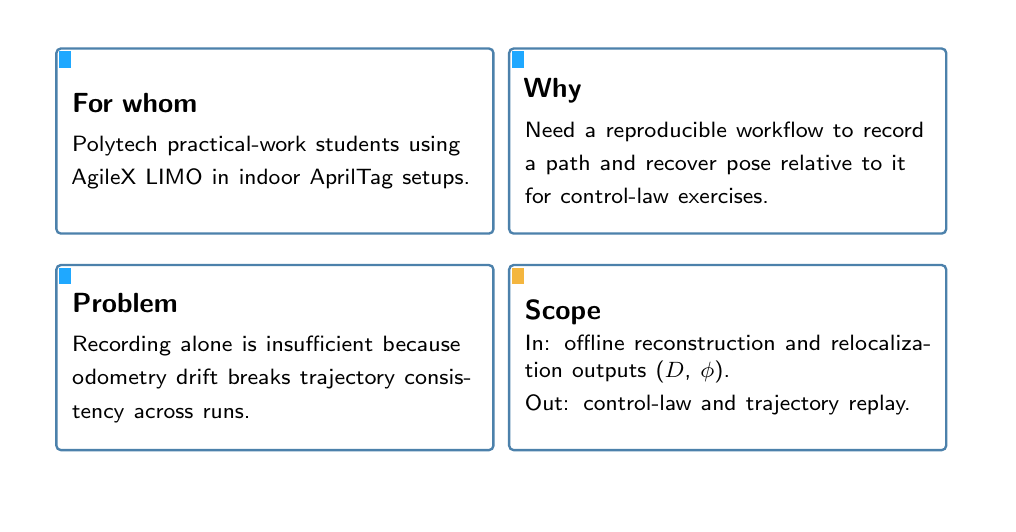
\begin{tikzpicture}[x=1cm,y=1cm]
  \fill[white] (0.2,0.3) rectangle (12.4,6.35);

  % Top-left card
  \node[visible on=<1->, draw=NavyBlue!70, fill=white, rounded corners=1.6pt, line width=0.85pt,
        anchor=north west, minimum width=5.55cm, minimum height=2.35cm, text width=5.15cm, align=left] (c1)
        at (0.55,6.10) {\textbf{For whom}\par\vspace{0.08cm}\footnotesize Polytech practical-work students using AgileX LIMO in indoor AprilTag setups.};
  \fill<1->[AccentBlue] ($(c1.north west)+(0.05,-0.05)$) rectangle ($(c1.north west)+(0.20,-0.26)$);
  \node<1->[anchor=west, text=white, font=\scriptsize\bfseries] at ($(c1.north west)+(0.08,-0.15)$) {1};

  % Top-right card
  \node[visible on=<2->, draw=NavyBlue!70, fill=white, rounded corners=1.6pt, line width=0.85pt,
        anchor=north west, minimum width=5.55cm, minimum height=2.35cm, text width=5.15cm, align=left] (c2)
        at (6.30,6.10) {\textbf{Why}\par\vspace{0.08cm}\footnotesize Need a reproducible workflow to record a path and recover pose relative to it for control-law exercises.};
  \fill<2->[AccentBlue] ($(c2.north west)+(0.05,-0.05)$) rectangle ($(c2.north west)+(0.20,-0.26)$);
  \node<2->[anchor=west, text=white, font=\scriptsize\bfseries] at ($(c2.north west)+(0.08,-0.15)$) {2};

  % Bottom-left card
  \node[visible on=<3->, draw=NavyBlue!70, fill=white, rounded corners=1.6pt, line width=0.85pt,
        anchor=north west, minimum width=5.55cm, minimum height=2.35cm, text width=5.15cm, align=left] (c3)
        at (0.55,3.35) {\textbf{Problem}\par\vspace{0.08cm}\footnotesize Recording alone is insufficient because odometry drift breaks trajectory consistency across runs.};
  \fill<3->[AccentBlue] ($(c3.north west)+(0.05,-0.05)$) rectangle ($(c3.north west)+(0.20,-0.26)$);
  \node<3->[anchor=west, text=white, font=\scriptsize\bfseries] at ($(c3.north west)+(0.08,-0.15)$) {3};

  % Bottom-right card
  \node[visible on=<4->, draw=NavyBlue!70, fill=white, rounded corners=1.6pt, line width=0.85pt,
        anchor=north west, minimum width=5.55cm, minimum height=2.35cm, text width=5.15cm, align=left] (c4)
        at (6.30,3.35) {\textbf{Scope}\par\vspace{0.06cm}\footnotesize In: offline reconstruction and relocalization outputs ($D$, $\phi$).\par\footnotesize Out: control-law and trajectory replay.};
  \fill<4->[AccentGold] ($(c4.north west)+(0.05,-0.05)$) rectangle ($(c4.north west)+(0.20,-0.26)$);
  \node<4->[anchor=west, text=white, font=\scriptsize\bfseries] at ($(c4.north west)+(0.08,-0.15)$) {4};

  % (No connectors, by design)
\end{tikzpicture}
\end{center}
\end{frame}

\begin{frame}[label=slide-setup]{Setup}
	\vspace{-0.20cm}
\begin{outlinecard}[Real Environment]
  \begin{columns}[T,onlytextwidth]
    \begin{column}{0.5\textwidth}
      \centering
      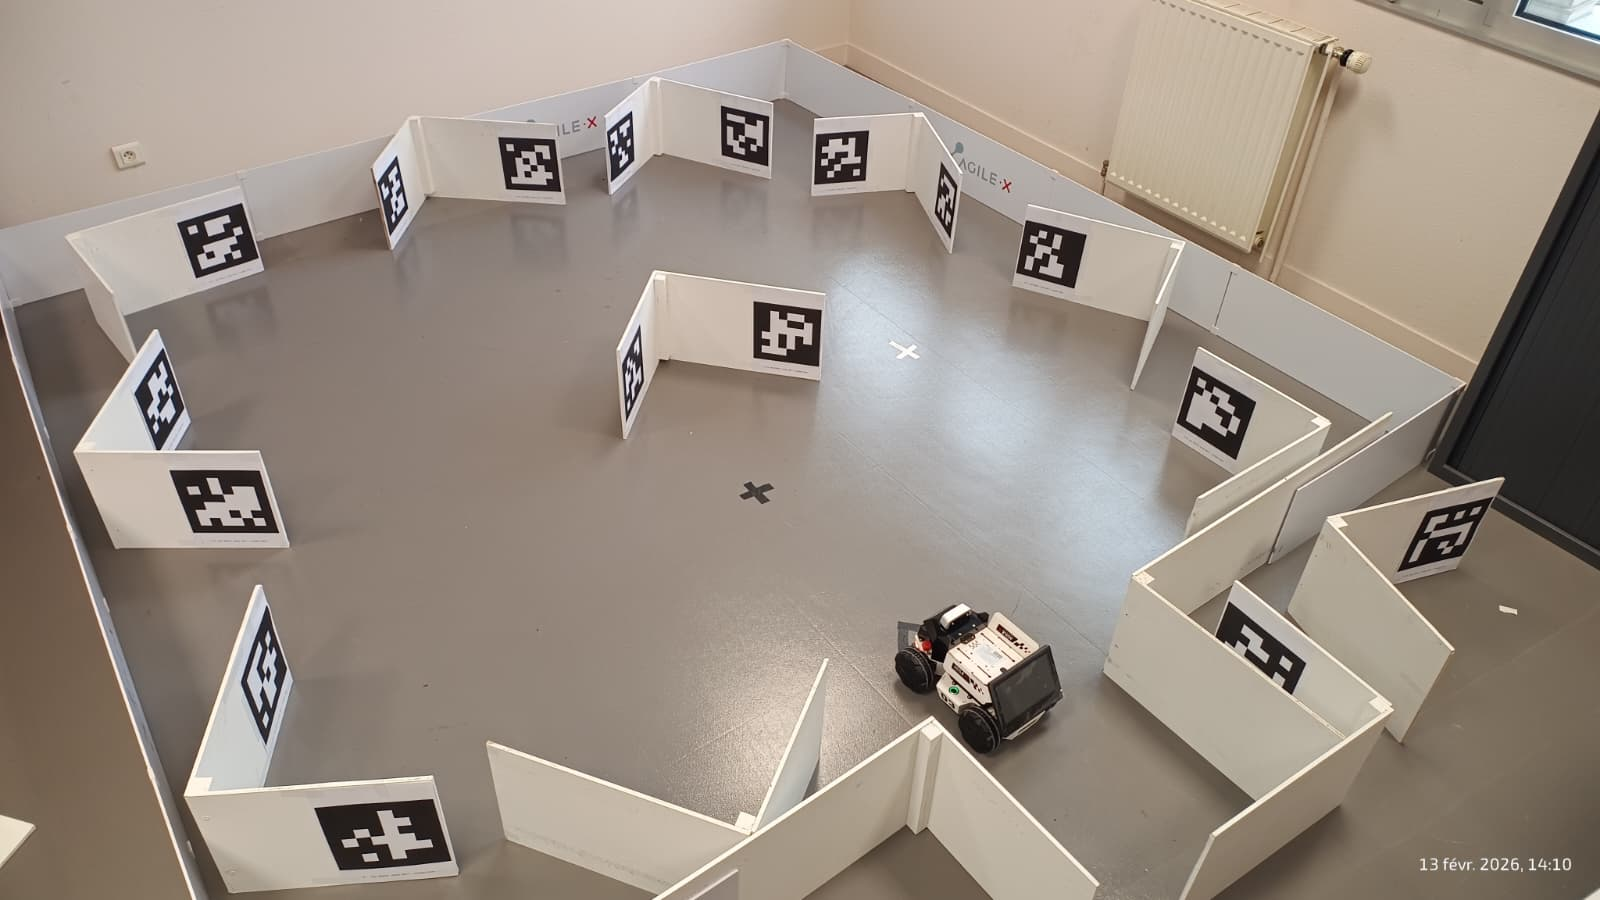
\includegraphics[width=0.96\linewidth,height=0.35\textheight,keepaspectratio]{../Report/Images/limo_real_environment.png}\\[-0.4mm]
      {\tiny Real setup with LIMO and AprilTags}
    \end{column}
    \begin{column}{0.5\textwidth}
      \centering
      \only<2->{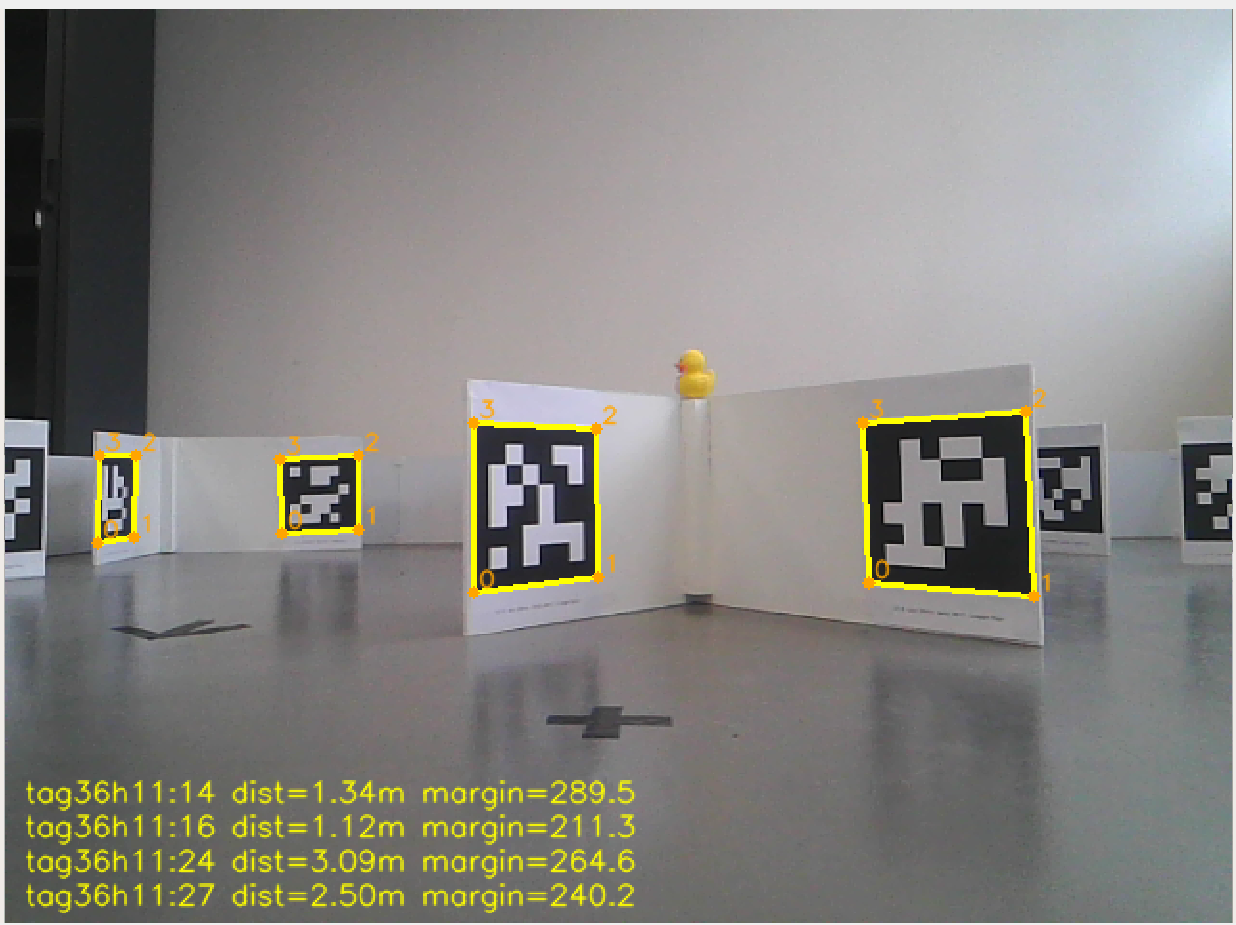
\includegraphics[width=0.96\linewidth,height=0.35\textheight,keepaspectratio]{assets/detections.png}\\[-0.4mm]}
      \only<2->{\tiny Detection's frame }
    \end{column}
  \end{columns}
\end{outlinecard}

\vspace{-0.12cm}
\begin{outlinecard}[Setup Flow]
  \centering
  \begin{tikzpicture}[x=1cm,y=1cm,>=Latex]
    % steps
    \node<1->[draw=NavyBlue!70, fill=white, rounded corners=1.2pt, line width=0.75pt,
      minimum width=2.70cm, minimum height=0.86cm, align=center] (s1) at (1.55,0.90)
      {\scriptsize\textbf{1) Drive}};
    \node<2->[draw=NavyBlue!70, fill=white, rounded corners=1.2pt, line width=0.75pt,
      minimum width=2.70cm, minimum height=0.86cm, align=center] (s2) at (4.65,0.90)
      {\scriptsize\textbf{2) Record}};
    \node<3->[draw=NavyBlue!70, fill=white, rounded corners=1.2pt, line width=0.75pt,
      minimum width=2.70cm, minimum height=0.86cm, align=center] (s3) at (7.75,0.90)
      {\scriptsize\textbf{3) Optimize}};
    \node<4->[draw=NavyBlue!70, fill=white, rounded corners=1.2pt, line width=0.75pt,
      minimum width=2.70cm, minimum height=0.86cm, align=center] (s4) at (10.85,0.90)
      {\scriptsize\textbf{4) Export}};

    % active marker
    \fill<1>[AccentGold] ($(s1.north west)+(0.04,-0.04)$) rectangle ($(s1.north west)+(0.15,-0.33)$);
    \fill<2>[AccentGold] ($(s2.north west)+(0.04,-0.04)$) rectangle ($(s2.north west)+(0.15,-0.33)$);
    \fill<3>[AccentGold] ($(s3.north west)+(0.04,-0.04)$) rectangle ($(s3.north west)+(0.15,-0.33)$);
    \fill<4>[AccentGold] ($(s4.north west)+(0.04,-0.04)$) rectangle ($(s4.north west)+(0.15,-0.33)$);

    % arrows
    \draw<2->[NavyBlue!60, line width=0.8pt, -{Latex[length=1.8mm,width=1.3mm]}] (2.9,0.90) -- (3.3,0.90);
    \draw<3->[NavyBlue!60, line width=0.8pt, -{Latex[length=1.8mm,width=1.3mm]}] (6.0,0.90) -- (6.4,0.90);
    \draw<4->[NavyBlue!60, line width=0.8pt, -{Latex[length=1.8mm,width=1.3mm]}] (9.1,0.90) -- (9.5,0.90);

    % visual icons above each step
    % 1) joystick
    \begin{scope}[visible on=<1->]
      \fill[AccentBlue!20] (1.55,1.30) circle (0.16);
      \draw[NavyBlue, line width=0.7pt] (1.55,1.30) circle (0.16);
      \node[text=NavyBlue, font=\scriptsize] at (1.55,1.30) {\faGamepad};
    \end{scope}

    % 2) rosbag database
    \begin{scope}[visible on=<2->]
      \fill[AccentBlue!20] (4.65,1.30) circle (0.16);
      \draw[NavyBlue, line width=0.7pt] (4.65,1.30) circle (0.16);
      \node[text=NavyBlue, font=\scriptsize] at (4.65,1.30) {\faDatabase};
    \end{scope}

    % 3) optimize
    \begin{scope}[visible on=<3->]
      \fill[AccentBlue!20] (7.75,1.30) circle (0.16);
      \draw[NavyBlue, line width=0.7pt] (7.75,1.30) circle (0.16);
      \node[text=NavyBlue, font=\scriptsize] at (7.75,1.30) {\faCogs};
    \end{scope}

    % 4) export file
    \begin{scope}[visible on=<4->]
      \fill[AccentBlue!20] (10.85,1.30) circle (0.16);
      \draw[NavyBlue, line width=0.7pt] (10.85,1.30) circle (0.16);
      \node[text=NavyBlue, font=\scriptsize] at (10.85,1.30) {\faFile};
    \end{scope}
  \end{tikzpicture}
\end{outlinecard}

			\end{frame}

\begin{frame}[label=slide-method]{Method}
% Template only — Method
\ScopeBadge
\vspace{0.2cm}
\begin{outlinecard}[Method — Template]
\small
\textbf{To fill later:}
\begin{itemize}
  \item Objective of the method
  \item Pipeline blocks
  \item Main equations
  \item Expected outputs
\end{itemize}
\end{outlinecard}

\end{frame}



\begin{frame}[label=slide-recording]{Recording Phase}
% Fixed two-column storyboard:
% <1> Step 1 input video
% <2> Step 2A before optimization
% <3> Step 2B after optimization
% <4-> Step 3 final exported result

\vspace{-0.4cm}
\begin{columns}[T,onlytextwidth]
  % ---------------- LEFT: VISUAL PANEL (changes by step) ----------------
  \begin{column}{0.63\textwidth}
    \begin{outlinecard}[{\only<1>{Input Recording Run}\only<2>{Build Map}\only<3>{ Optimization}\only<4->{Optimized with Tf}}]
      \centering

% STEP 1
      \only<1>{
        \begin{tikzpicture}[x=1cm,y=1cm]
          \draw[draw=NavyBlue!45, line width=0.9pt, rounded corners=1.4pt, fill=white]
            (0.10,0.22) rectangle (7.3,3.9);
          % fixed inner media area (keeps image inside frame)
          \node[inner sep=0pt, anchor=south west] at (0.33,0.50)
          {%
            \IfFileExists{assets/videotrack_fixed_traj_4x.mp4}{%
              \movie[
                width=6.6cm,
                height=3.20cm,
                poster
              ]{%
                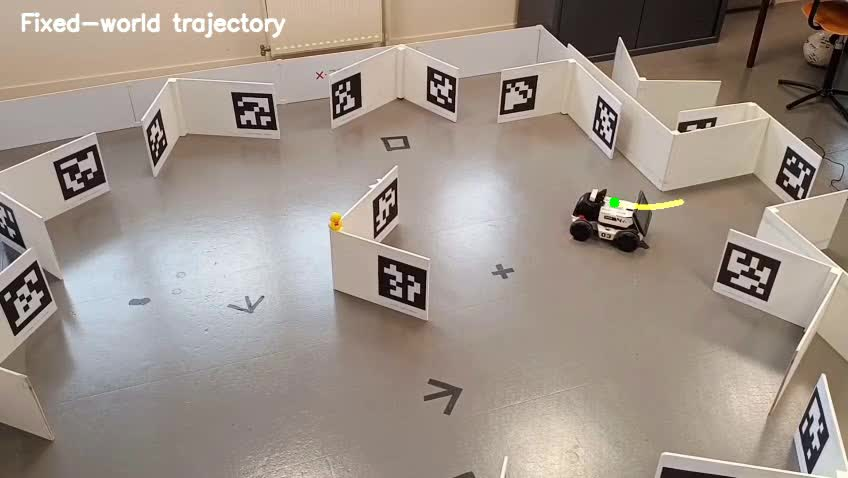
\includegraphics[
                  width=6.6cm,
                  height=3.20cm
                ]{assets/videotrack_fixed_traj_thumb.jpg}%
              }{assets/videotrack_fixed_traj_4x.mp4}%
            }{%
              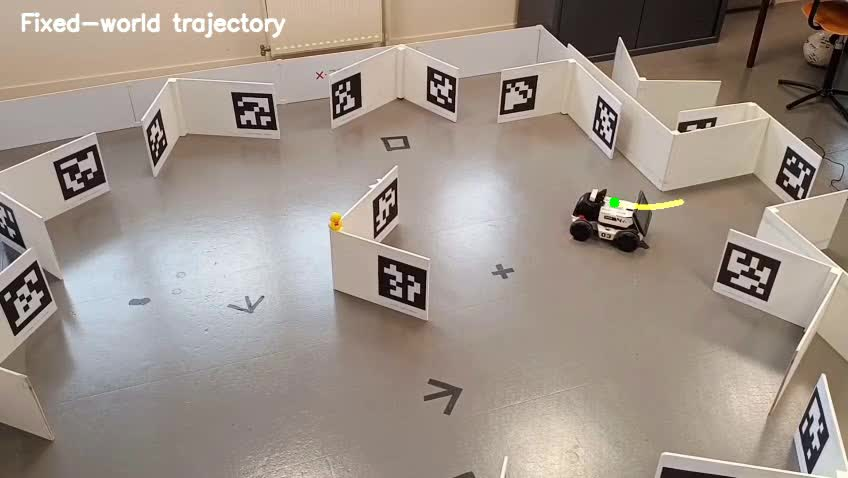
\includegraphics[width=6.6cm,height=3.20cm]{assets/videotrack_fixed_traj_thumb.jpg}%
            }%
          };
          \fill[black, opacity=0.18] (0.33,0.50) rectangle (6.93,3.70);
          \fill[white, opacity=0.92] (3.72,2.10) circle (0.30);
          \fill[NavyBlue] (3.63,1.98) -- (3.63,2.22) -- (3.84,2.10) -- cycle;
        \end{tikzpicture}
      }

      % STEP 2A
      \only<2>{
        \begin{tikzpicture}[x=1cm,y=1cm]
          \node[inner sep=0pt, anchor=south west] at (0.12,0.24)
            {
\includegraphics[width=7cm,height=5cm]{../assets/results/recording_before_no_opt_anchor24.png}};
          \node[anchor=south east, inner sep=0pt] at (8.18,0.6){
            \begin{tikzpicture}[x=1cm,y=1cm]
              \draw[draw=NavyBlue!55, fill=white, rounded corners=0.8pt, line width=0.6pt] (0,0) rectangle (1.35,1.35);
              \draw[AccentBlue, line width=0.9pt] (0.10,1.12) -- (0.34,1.12);
              \node[anchor=west, font=\tiny] at (0.40,1.12) {trajectory};
              \fill[green!70!black] (0.10,0.88) circle (0.025);
              \fill[red!80!black]   (0.25,0.88) circle (0.025);
              \node[anchor=west, font=\tiny] at (0.36,0.88) {start/end};
              \fill[AccentGold] (0.10,0.64) circle (0.025);
              \node[anchor=west, font=\tiny] at (0.20,0.64) {tags};
              \fill[AccentGold] (0.10,0.40) circle (0.033);
              \draw[black, line width=0.4pt] (0.10,0.40) circle (0.033);
              \node[anchor=west, font=\tiny] at (0.20,0.40) {anchor};
              \fill[AccentBlue!45] (0.10,0.16) circle (0.025);
              \node[anchor=west, font=\tiny] at (0.20,0.16) {cloud};
            \end{tikzpicture}
          };
        \end{tikzpicture}
      }

      % STEP 2B
      \only<3>{
        \begin{tikzpicture}[x=1cm,y=1cm]
          \node[inner sep=0pt, anchor=south west] at (0.12,0.2)
            {
\includegraphics[width=7cm,height=5cm]{../assets/results/recording_after_opt_anchor24.png}};
          \node[anchor=south east, inner sep=0pt] at (8.18,0.6){
            \begin{tikzpicture}[x=1cm,y=1cm]
              \draw[draw=NavyBlue!55, fill=white, rounded corners=0.8pt, line width=0.6pt] (0,0) rectangle (1.35,1.12);
              \draw[AccentBlue, line width=0.9pt] (0.10,0.90) -- (0.34,0.90);
              \node[anchor=west, font=\tiny] at (0.40,0.90) {trajectory};
              \fill[green!70!black] (0.10,0.66) circle (0.025);
              \fill[red!80!black]   (0.25,0.66) circle (0.025);
              \node[anchor=west, font=\tiny] at (0.36,0.66) {start/end};
              \fill[AccentGold] (0.10,0.42) circle (0.025);
              \node[anchor=west, font=\tiny] at (0.20,0.42) {tags};
              \fill[AccentGold] (0.10,0.18) circle (0.033);
              \draw[black, line width=0.4pt] (0.10,0.18) circle (0.033);
              \node[anchor=west, font=\tiny] at (0.20,0.18) {anchor};
            \end{tikzpicture}
          };
        \end{tikzpicture}
      }

      % STEP 3
      \only<4->{
        \begin{tikzpicture}[x=1cm,y=1cm]
          \node[inner sep=0pt, anchor=south west] at (0.12,0.24)
            {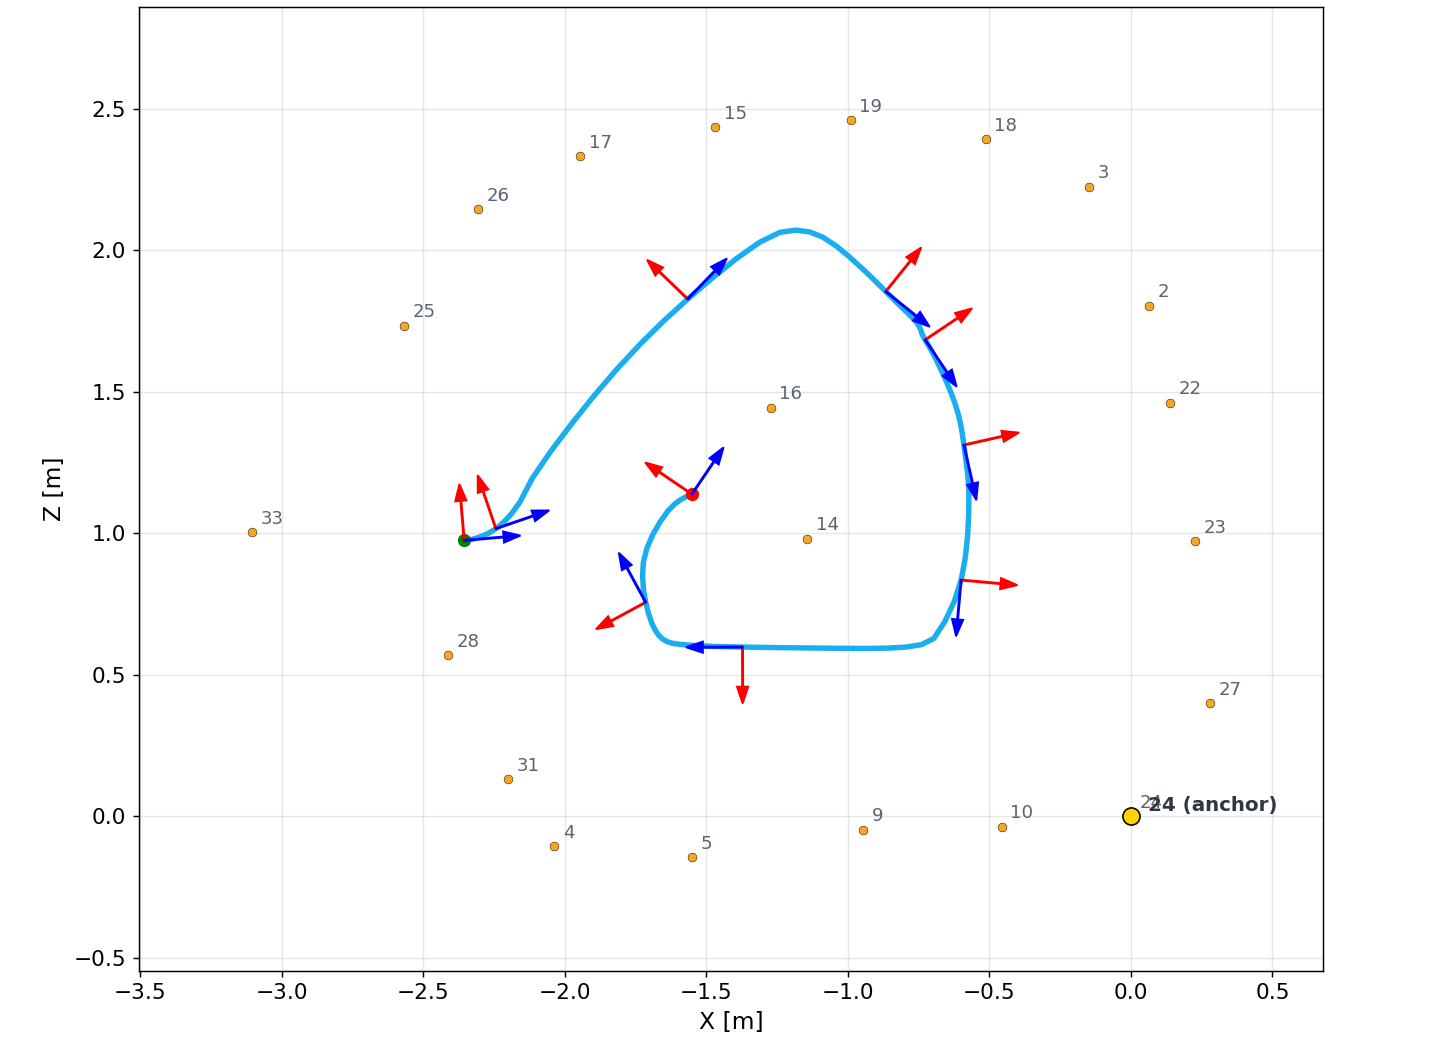
\includegraphics[width=7cm,height=5cm]{../assets/results/recording_final_opt_with_tf_anchor24.png}};
          \node[anchor=south east, inner sep=0pt] at (8.18,0.6){
            \begin{tikzpicture}[x=1cm,y=1cm]
              \draw[draw=NavyBlue!55, fill=white, rounded corners=0.8pt, line width=0.6pt] (0,0) rectangle (1.45,1.35);
              \draw[AccentBlue, line width=0.9pt] (0.10,1.12) -- (0.34,1.12);
              \node[anchor=west, font=\tiny] at (0.40,1.12) {trajectory};
              \fill[green!70!black] (0.10,0.88) circle (0.025);
              \fill[red!80!black]   (0.25,0.88) circle (0.025);
              \node[anchor=west, font=\tiny] at (0.36,0.88) {start/end};
              \fill[AccentGold] (0.10,0.64) circle (0.025);
              \node[anchor=west, font=\tiny] at (0.20,0.64) {tags};
              \fill[AccentGold] (0.10,0.40) circle (0.033);
              \draw[black, line width=0.4pt] (0.10,0.40) circle (0.033);
              \node[anchor=west, font=\tiny] at (0.20,0.40) {anchor};
              \draw[red,  line width=0.7pt, -{Latex[length=1.1mm]}] (0.10,0.16) -- (0.34,0.16);
              \draw[blue, line width=0.7pt, -{Latex[length=1.1mm]}] (0.10,0.16) -- (0.10,0.39);
              \node[anchor=west, font=\tiny] at (0.40,0.16) {axes};
            \end{tikzpicture}
          };
        \end{tikzpicture}
      }
    \end{outlinecard}
  \end{column}

  % ---------------- RIGHT: VERTICAL PIPELINE (always visible) ----------------
  \begin{column}{0.35\textwidth}
    \begin{outlinecard}[Pipeline]
      \centering
      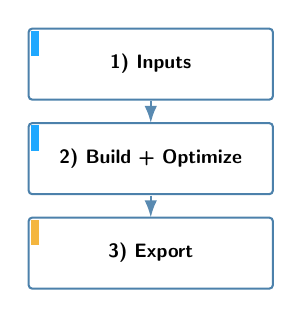
\begin{tikzpicture}[x=1cm,y=1cm,>=Latex]
        \node<1->[draw=NavyBlue!70, fill=white, rounded corners=1.2pt, line width=0.75pt,
          minimum width=3.10cm, minimum height=0.90cm, align=center] (p1) at (1.6,3.05)
          {\scriptsize\textbf{1) Inputs}};
        \node<2->[draw=NavyBlue!70, fill=white, rounded corners=1.2pt, line width=0.75pt,
          minimum width=3.10cm, minimum height=0.90cm, align=center] (p2) at (1.6,1.85)
          {\scriptsize\textbf{2) Build + Optimize}};
        \node<4->[draw=NavyBlue!70, fill=white, rounded corners=1.2pt, line width=0.75pt,
          minimum width=3.10cm, minimum height=0.90cm, align=center] (p3) at (1.6,0.65)
          {\scriptsize\textbf{3) Export}};

        % active step marker
        \fill<1>[AccentGold] ($(p1.north west)+(0.04,-0.04)$) rectangle ($(p1.north west)+(0.15,-0.36)$);
        \fill<2-3>[AccentGold] ($(p2.north west)+(0.04,-0.04)$) rectangle ($(p2.north west)+(0.15,-0.36)$);
        \fill<4->[AccentGold] ($(p3.north west)+(0.04,-0.04)$) rectangle ($(p3.north west)+(0.15,-0.36)$);
        % non-active markers
        \fill<2->[AccentBlue] ($(p1.north west)+(0.04,-0.04)$) rectangle ($(p1.north west)+(0.15,-0.36)$);
        \fill<4->[AccentBlue] ($(p2.north west)+(0.04,-0.04)$) rectangle ($(p2.north west)+(0.15,-0.36)$);

        \draw<2->[NavyBlue!65, line width=0.9pt, -{Latex[length=2.2mm,width=1.6mm]}] (1.6,2.58) -- (1.6,2.30);
        \draw<4->[NavyBlue!65, line width=0.9pt, -{Latex[length=2.2mm,width=1.6mm]}] (1.6,1.38) -- (1.6,1.10);
      \end{tikzpicture}
    \end{outlinecard}

    \vspace{-0.2cm}
    \only<1>{
      \begin{outlinecard}[Step Notes]
        \scriptsize
        \textit{Data acquisition step with rosbag.}
      \end{outlinecard}
    }
    \only<2>{
      \begin{outlinecard}[Equation]
        \scriptsize
        \[
          {}^{\text{world}}\!T_{\mathrm{tag}_i}(t)
          =
          {}^{\text{world}}\!T_{\mathrm{cam}}(t)
          \;{}^{\text{cam}}\!T_{\mathrm{tag}_i}(t)
        \]
      \end{outlinecard}
    }
    \only<3>{
      \begin{outlinecard}[Optimization Equation]
        \scriptsize
        \[
          \min_{\{{}^{w}T_{\mathrm{tag}_i}\}}
          \sum_{(i,j)\in\mathcal{E}}
          \rho\!\left(\|\mathrm{err}_{ij}\|^2\right)
        \]
      \end{outlinecard}
    }
    \only<4->{
      \begin{outlinecard}[Exported Outputs]
        \scriptsize
        \begin{itemize}
          \item \texttt{tag\_map.yaml}
          \item \texttt{trajetoria\_camera.csv}
          \item \texttt{mapa\_tags.csv}
        \end{itemize}
      \end{outlinecard}
    }
  \end{column}
\end{columns}

\end{frame}

\begin{frame}[label=slide-relocalization]{Relocalization Phase}
% Relocalization phase storyboard:
% <1> Previous-phase reference (what is reused)
% <2> Captured point photos (replace paths)
% <3-> Didactic nearest-point graphs (replace paths)

\vspace{-0.3cm}
\begin{columns}[T,onlytextwidth]
  % ---------------- LEFT: VISUAL PANEL ----------------
  \begin{column}{0.63\textwidth}
    \begin{outlinecard}[{\only<1>{Recorded Reference}\only<2-7>{Point Validation (Photo + Graph)}}]
      \centering

      % STEP 1
      \only<1>{
        \begin{tikzpicture}[x=1cm,y=1cm]
          \draw[draw=NavyBlue!45, line width=0.9pt, rounded corners=1.4pt, fill=white]
            (0.10,0.22) rectangle (7.3,3.9);
          \node[inner sep=0pt, anchor=south west] at (0.30,0.44)
            {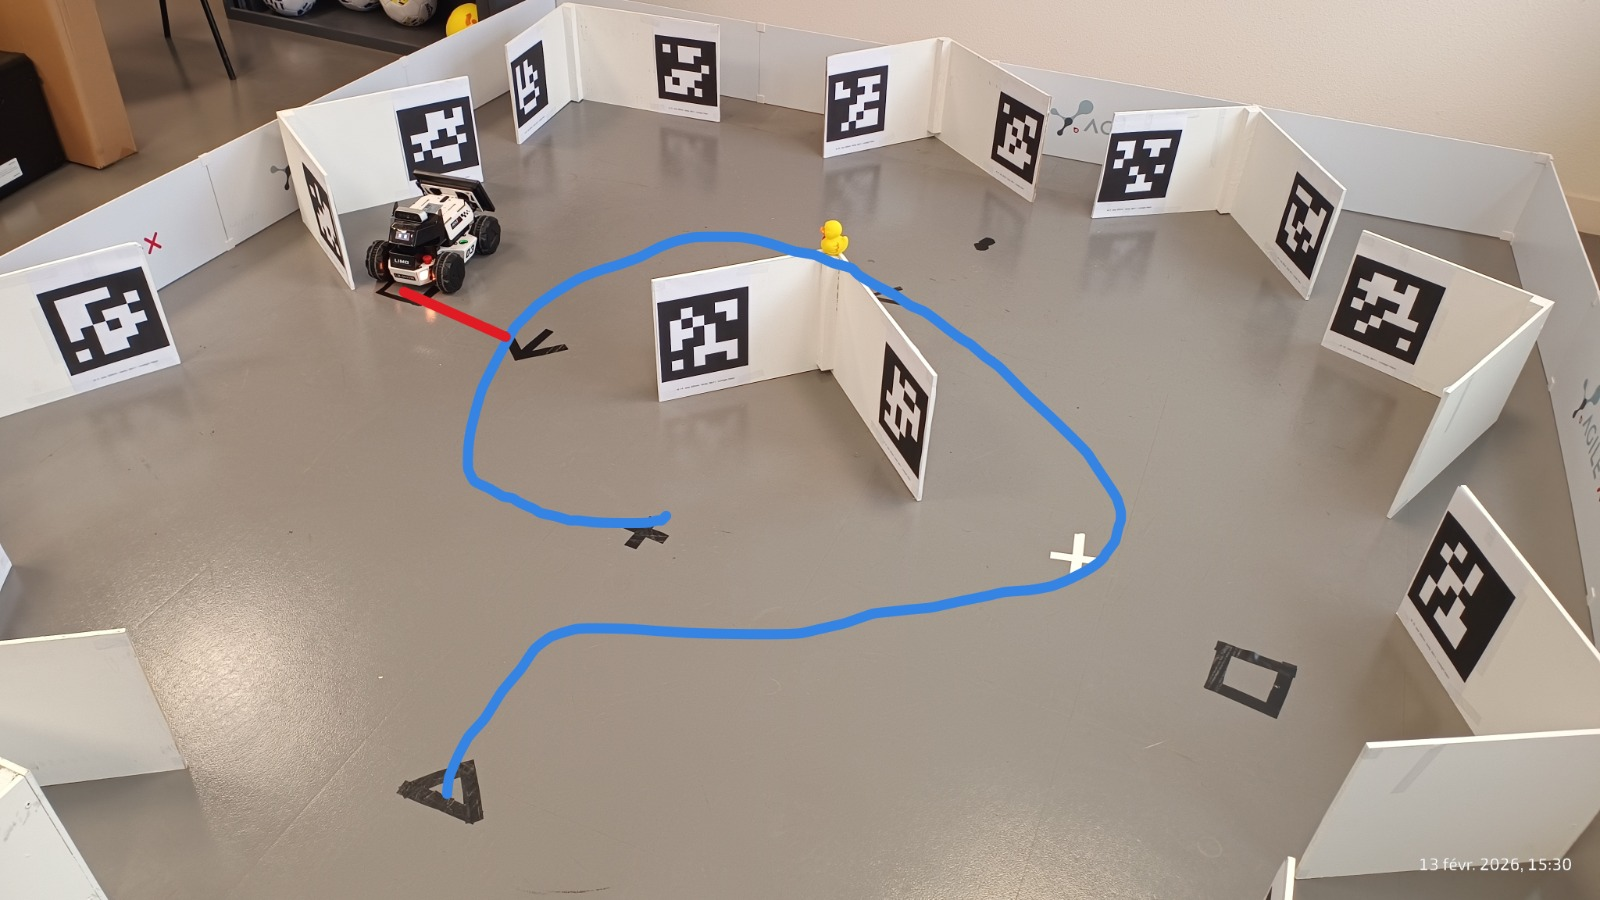
\includegraphics[width=6.7cm,height=3.25cm]{assets/relocphase_1.jpeg}};
          \fill[black, opacity=0.15] (0.30,0.44) rectangle (7.00,3.69);
        \end{tikzpicture}
      }

      % STEP 2
      \only<2-7>{
        \begin{tikzpicture}[x=1cm,y=1cm]
          % Pair 1: 002
          \only<2>{
            \node[anchor=south west, inner sep=0pt] at (0.30,0.34)
              {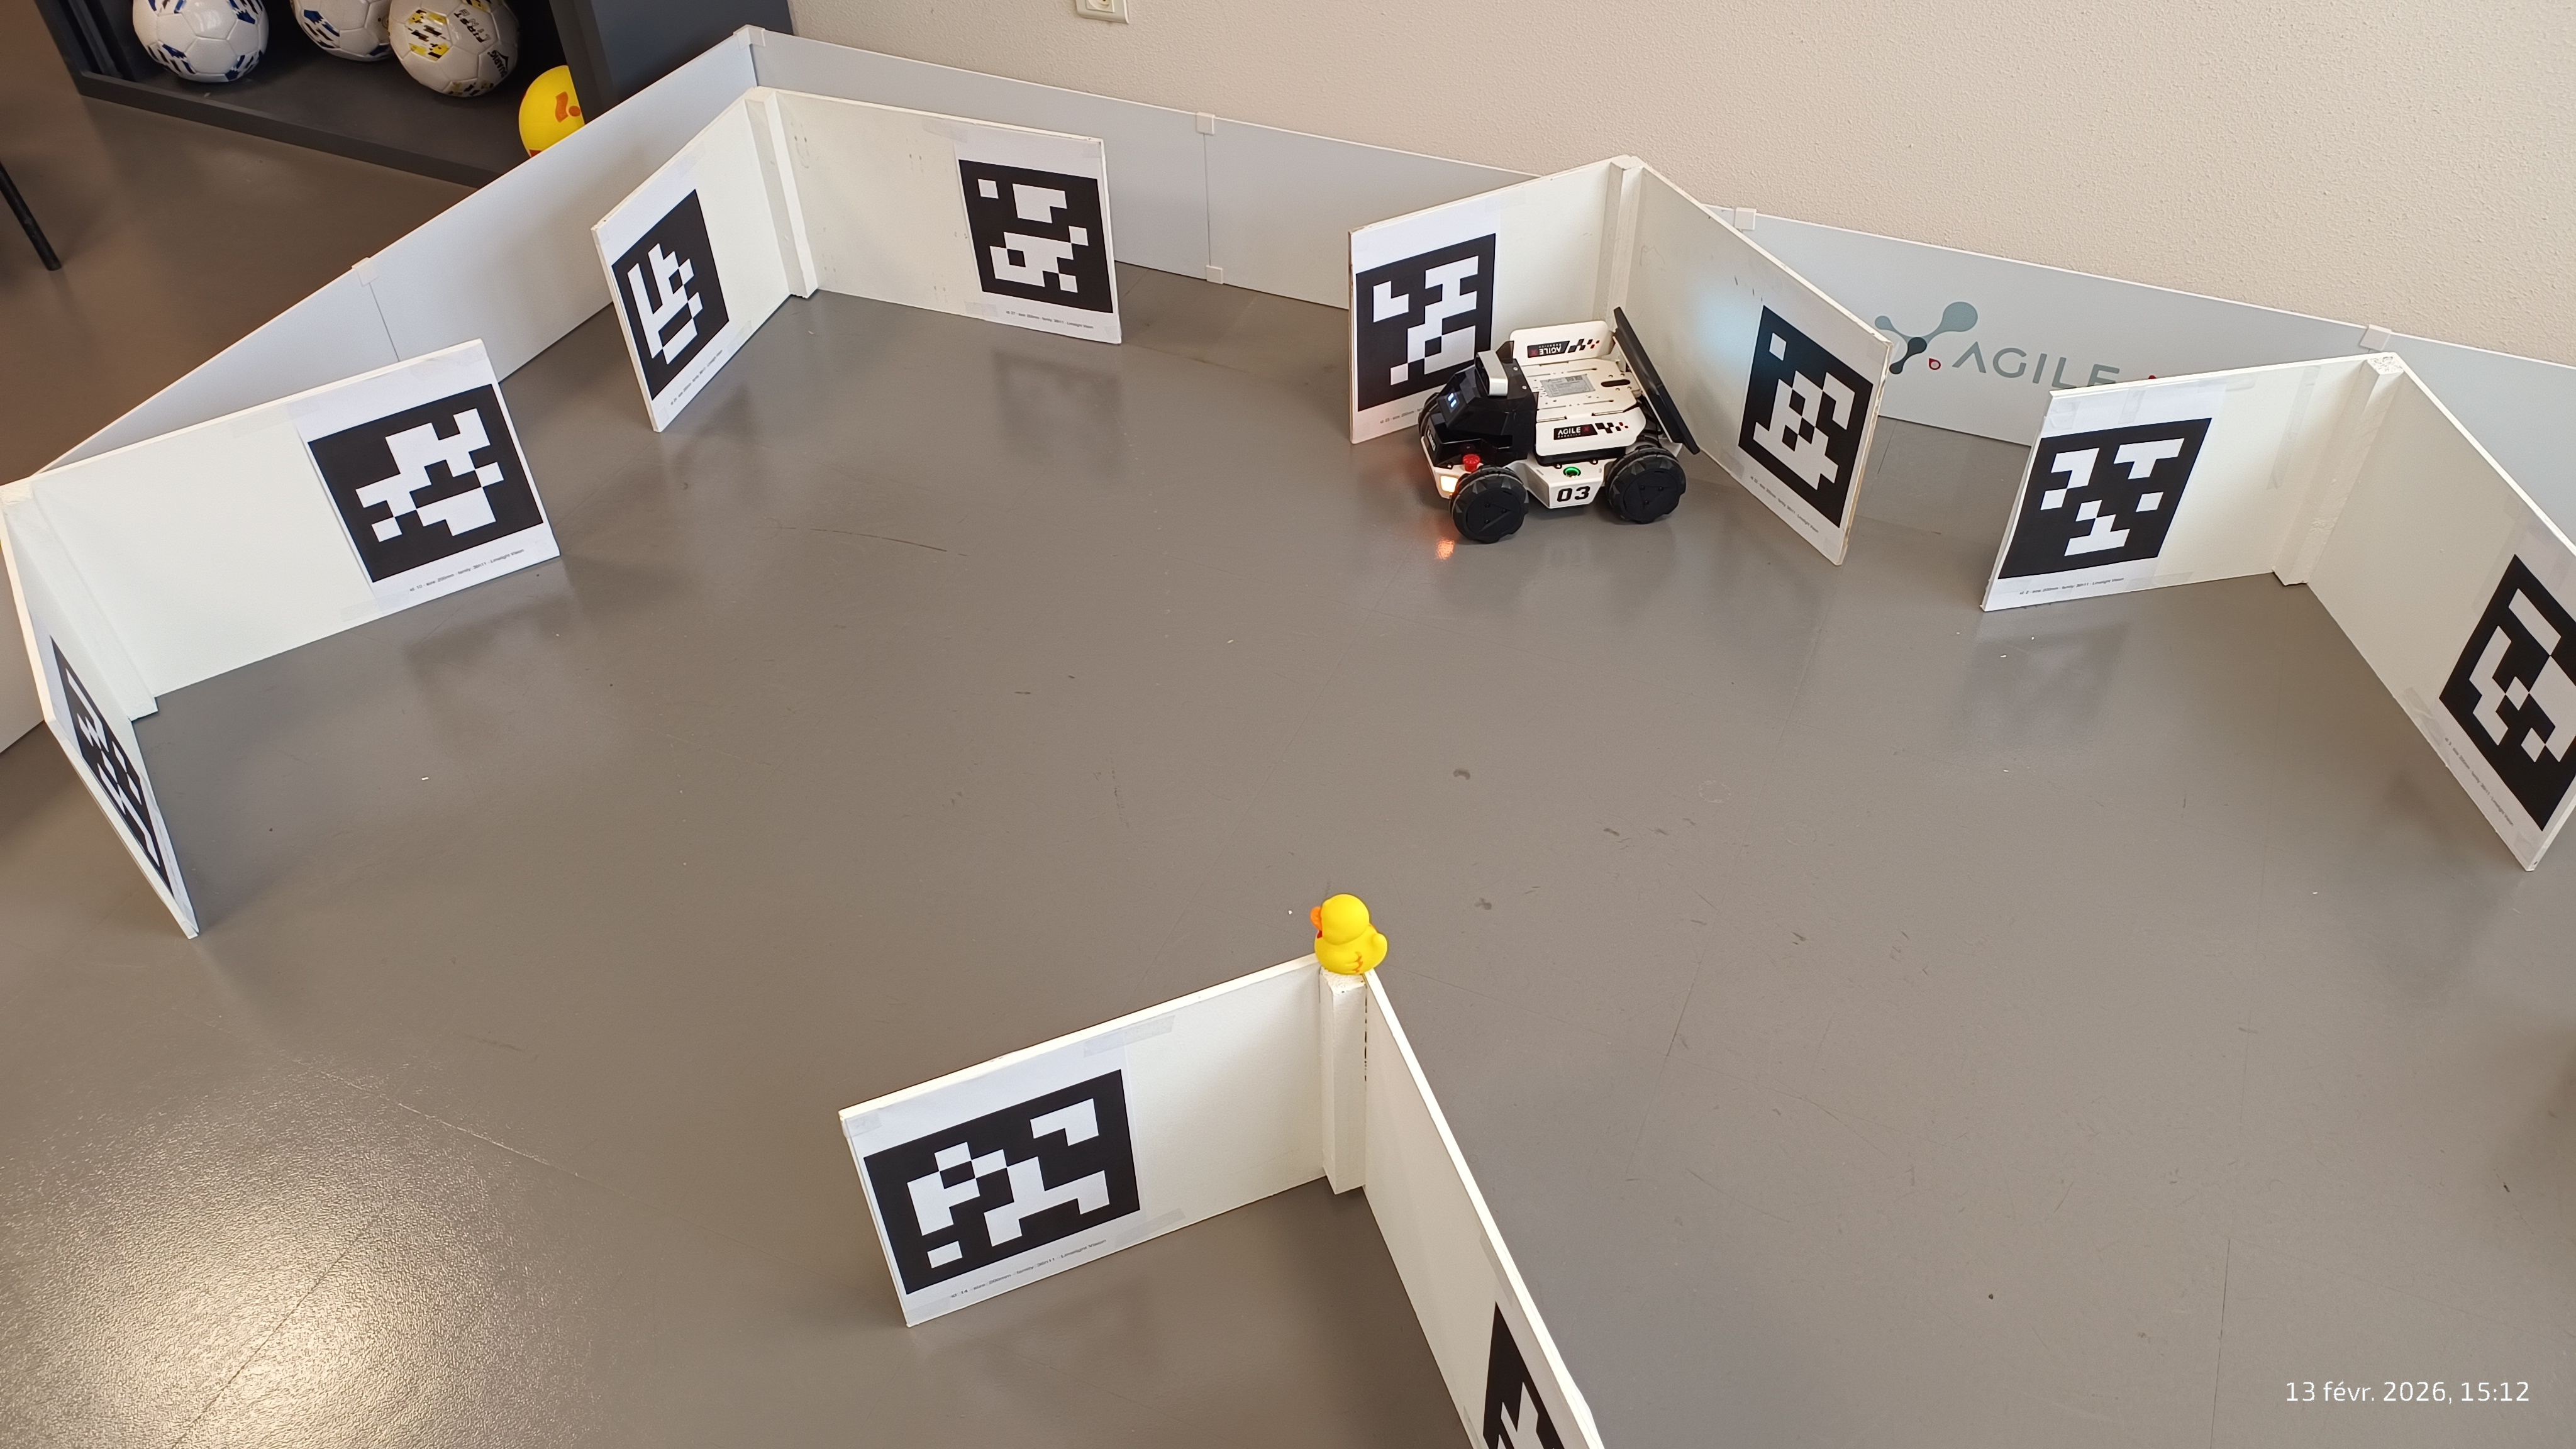
\includegraphics[width=3.35cm,height=3.30cm]{../assets/results/real_s1_reloc_002_foto.jpg}};
            \node[anchor=south west, inner sep=0pt] at (3.85,0.34)
              {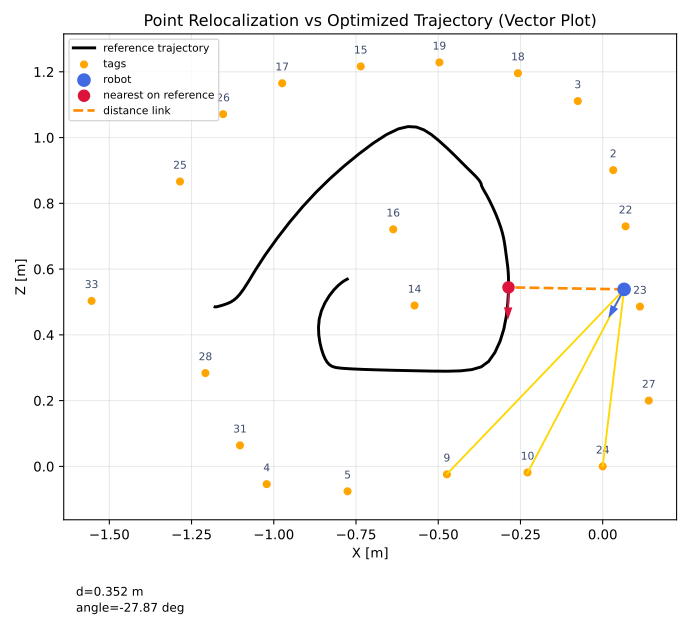
\includegraphics[width=3.35cm,height=3.30cm]{assets/results/graph_002.png}};
            \node[font=\scriptsize\bfseries, text=NavyBlue, anchor=north] at (1.98,0.30) {Point 002};
            \node[font=\scriptsize\bfseries, text=NavyBlue, anchor=north] at (5.53,0.30) {Graph 002};
          }
          % Pair 2: 012
          \only<3>{
            \node[anchor=south west, inner sep=0pt] at (0.30,0.34)
              {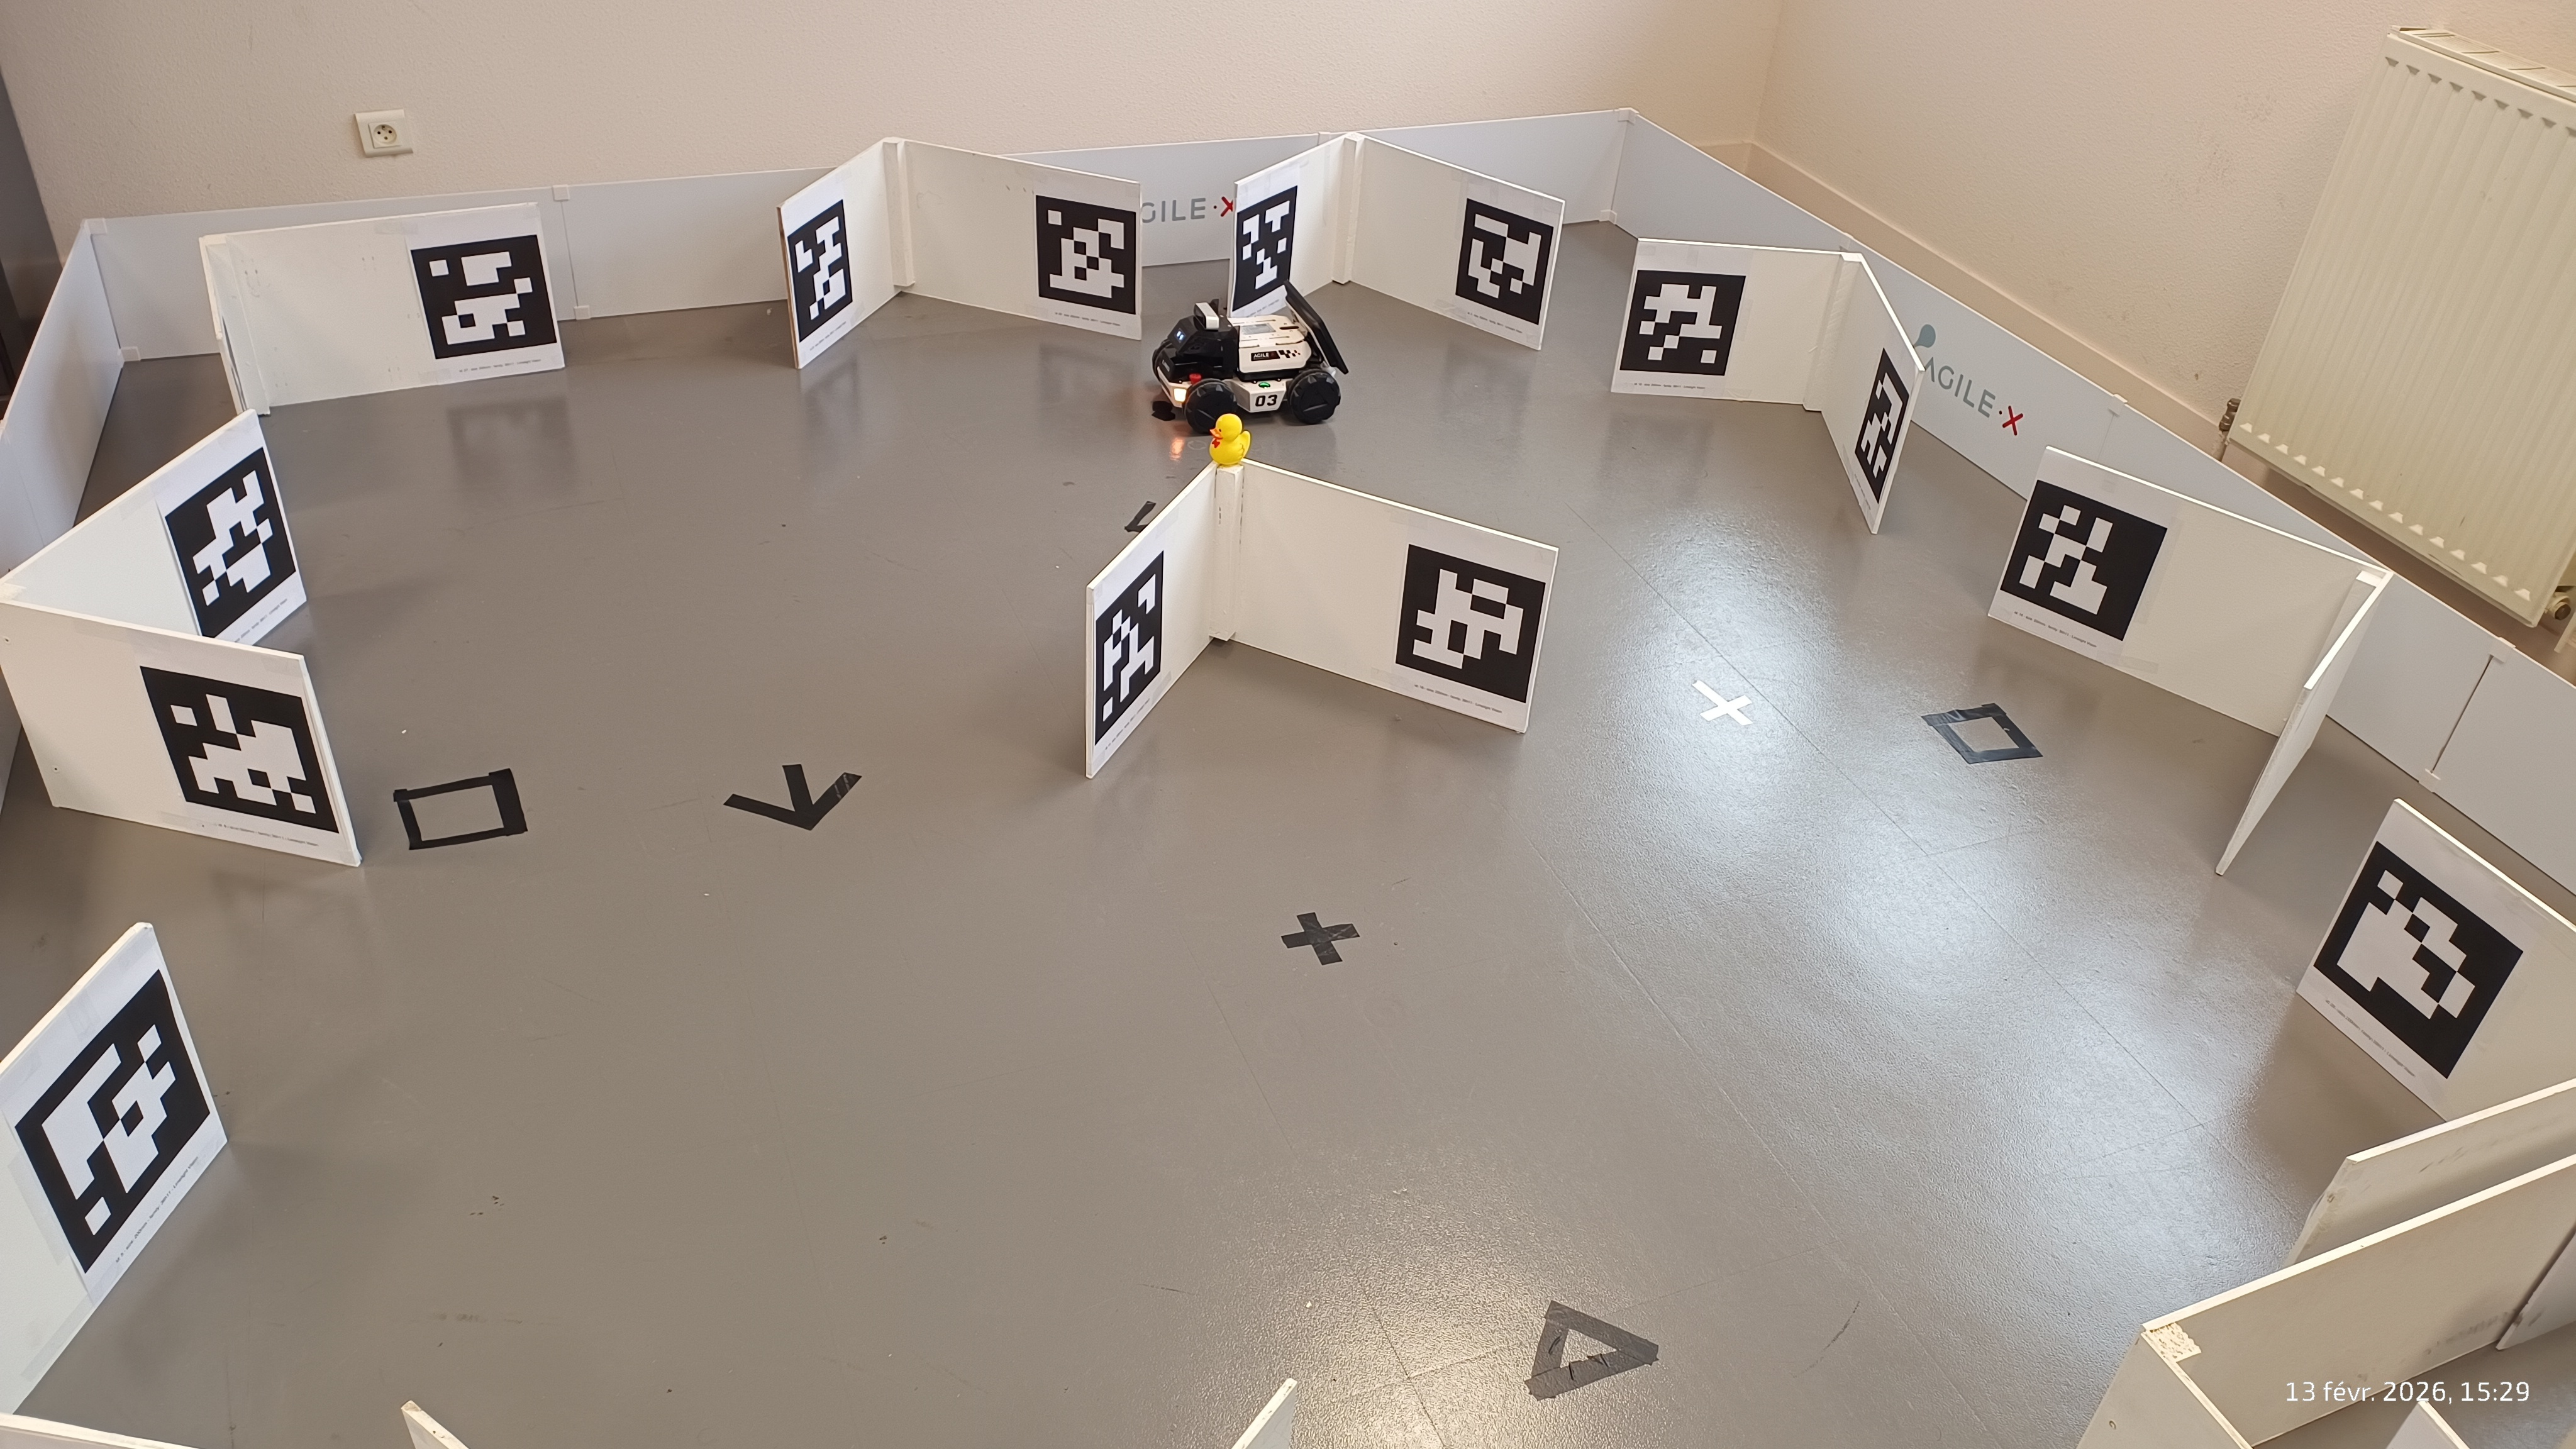
\includegraphics[width=3.35cm,height=3.30cm]{../assets/results/real_s1_reloc_012_foto.jpg}};
            \node[anchor=south west, inner sep=0pt] at (3.85,0.34)
              {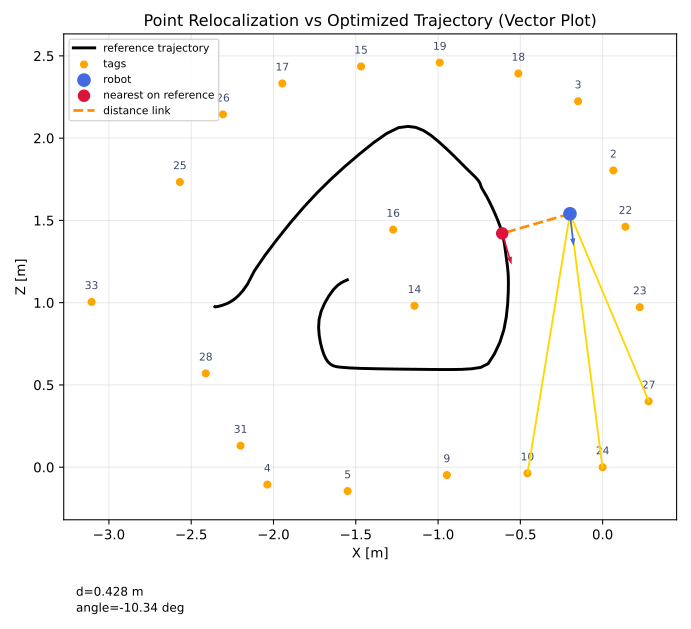
\includegraphics[width=3.35cm,height=3.30cm]{assets/results/graph_012.png}};
            \node[font=\scriptsize\bfseries, text=NavyBlue, anchor=north] at (1.98,0.30) {Point 012};
            \node[font=\scriptsize\bfseries, text=NavyBlue, anchor=north] at (5.53,0.30) {Graph 012};
          }
          % Pair 3: 013
          \only<4>{
            \node[anchor=south west, inner sep=0pt] at (0.30,0.34)
              {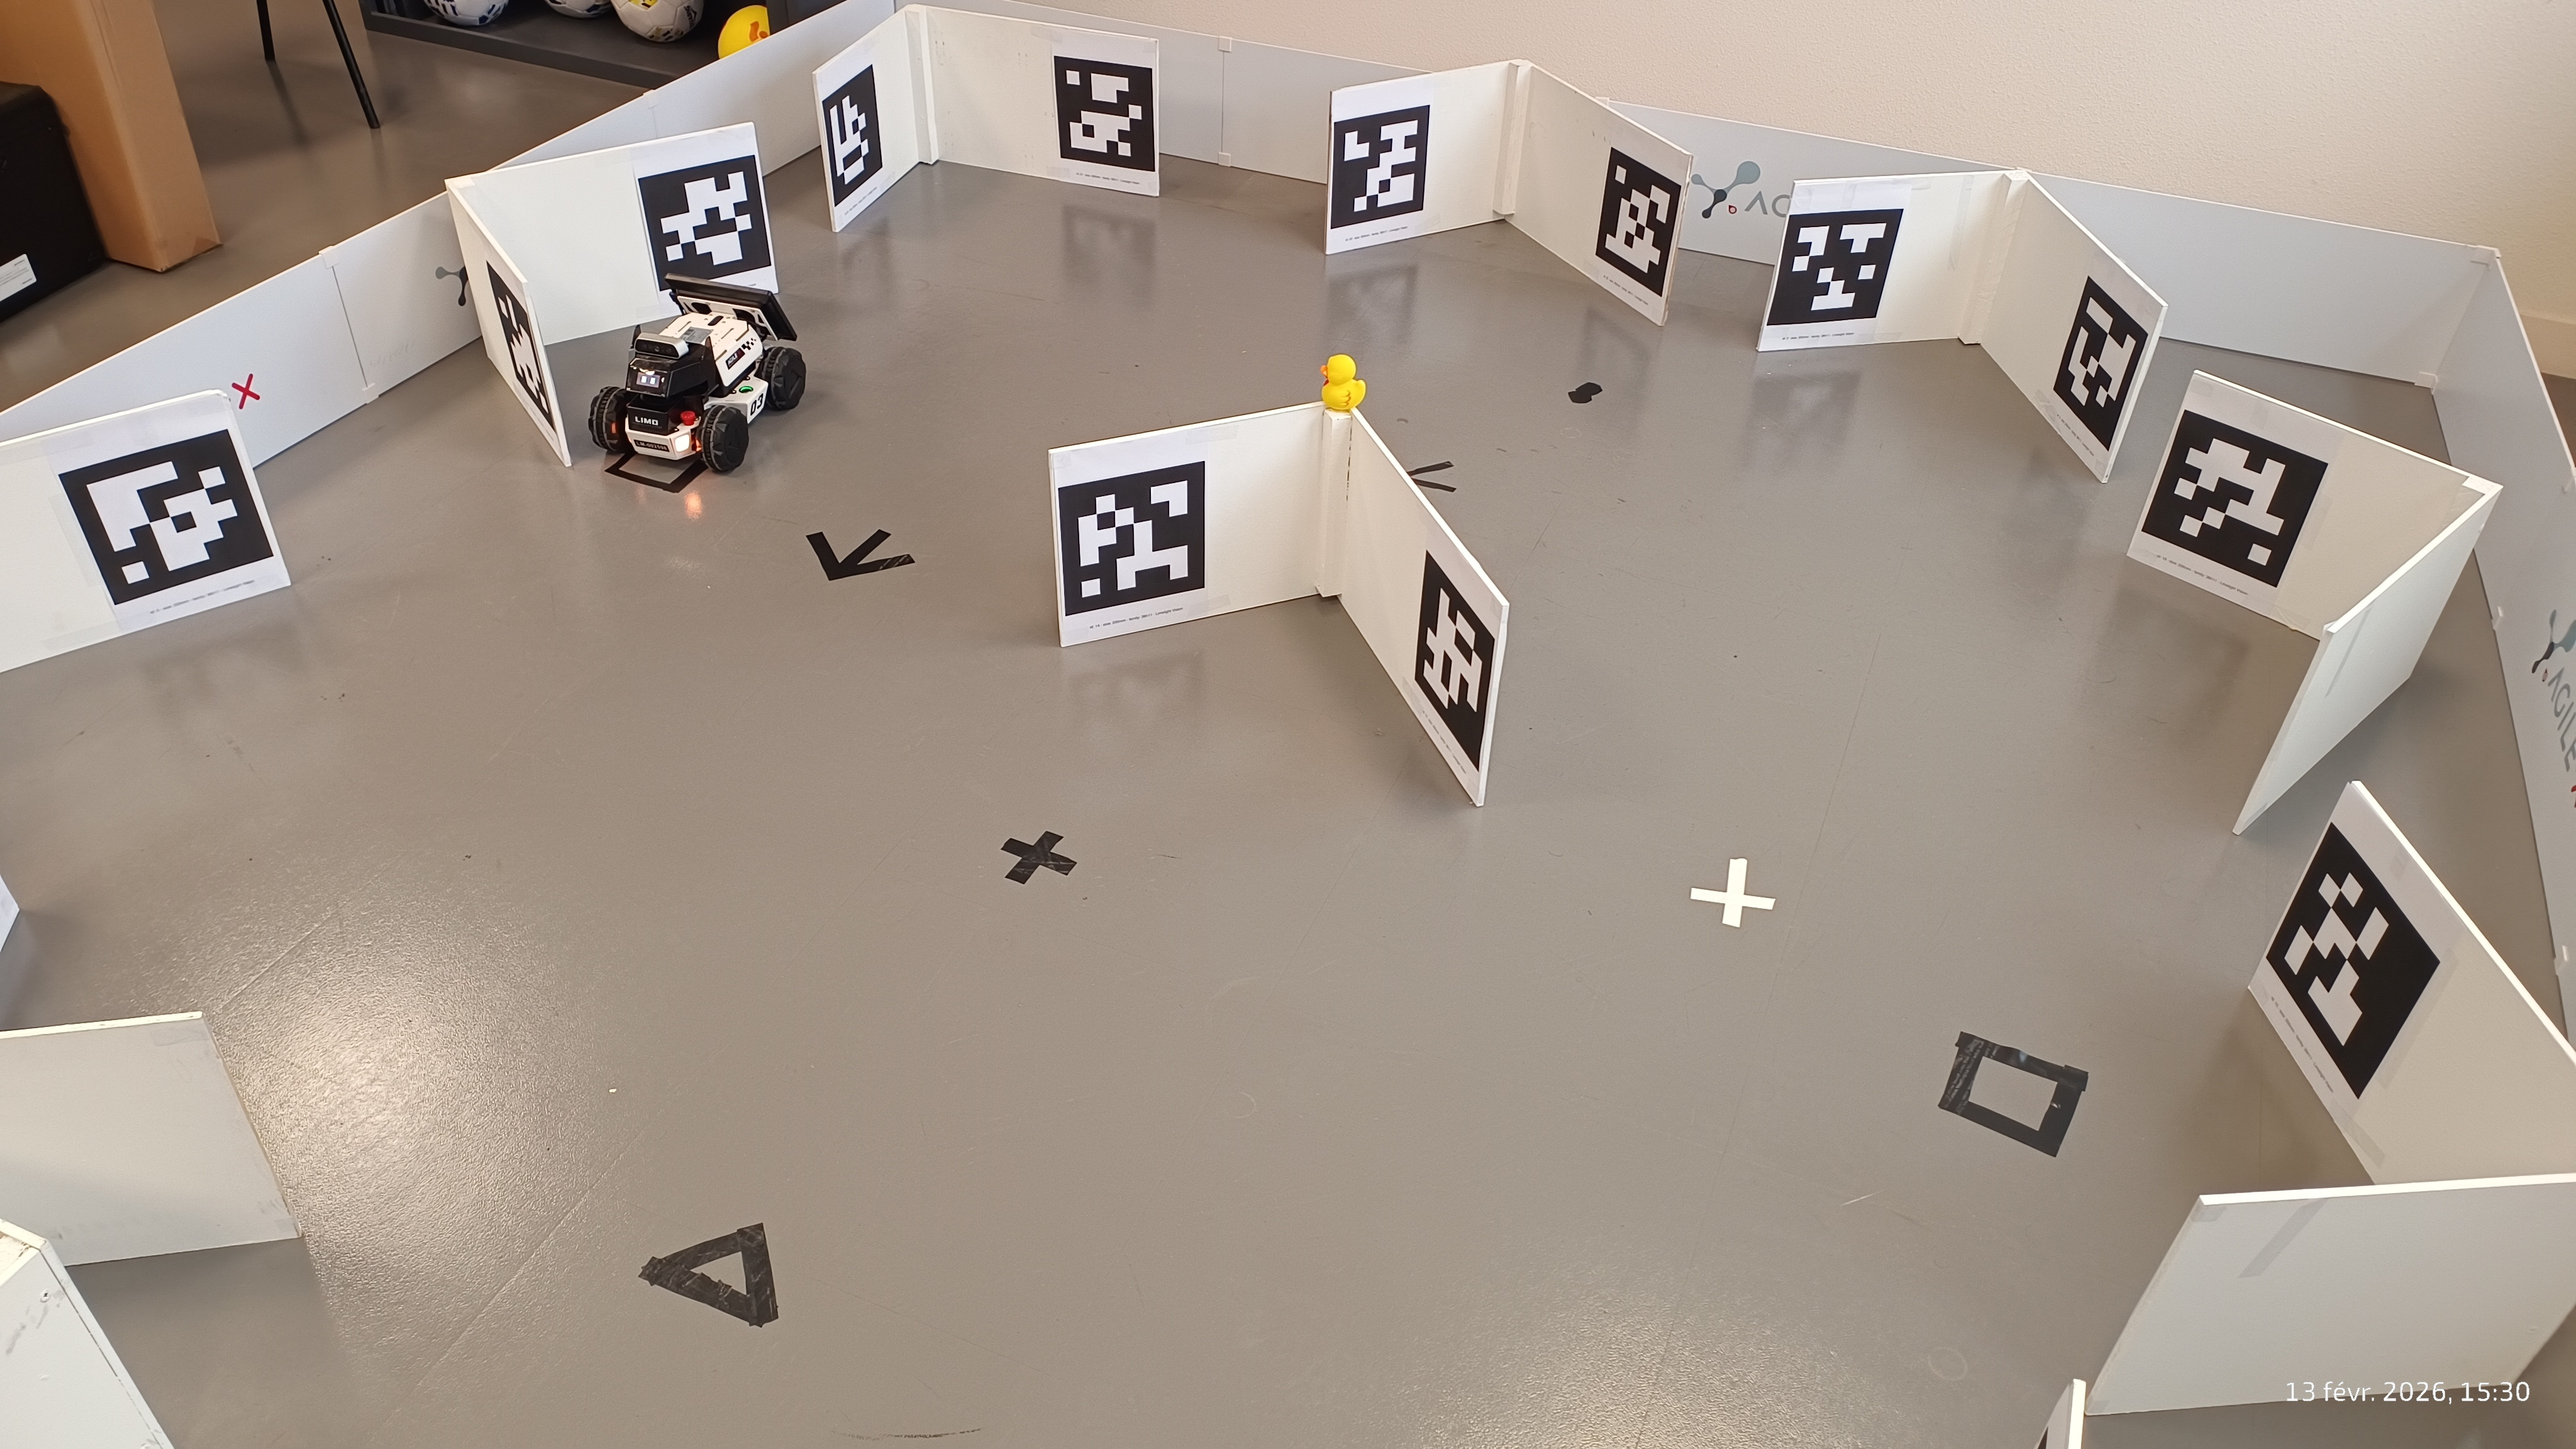
\includegraphics[width=3.35cm,height=3.30cm]{../assets/results/real_s1_reloc_13_foto.jpg}};
            \node[anchor=south west, inner sep=0pt] at (3.85,0.34)
              {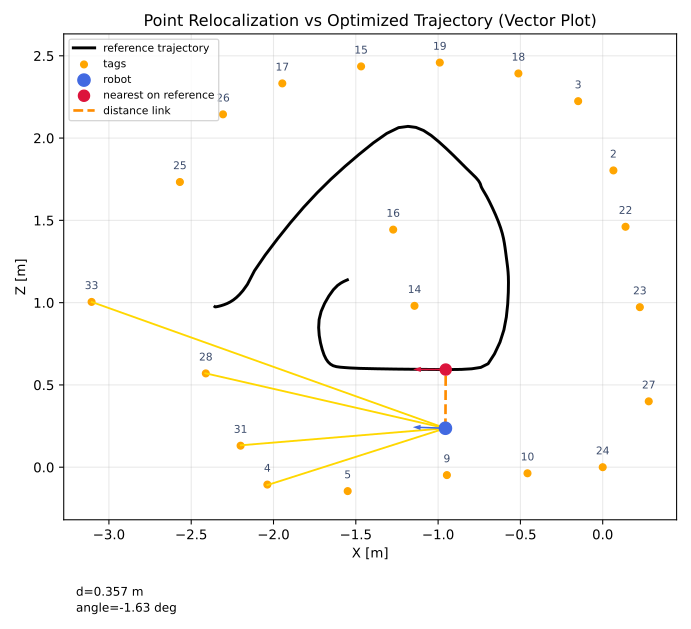
\includegraphics[width=3.35cm,height=3.30cm]{assets/results/graph_013.png}};
            \node[font=\scriptsize\bfseries, text=NavyBlue, anchor=north] at (1.98,0.30) {Point 013};
            \node[font=\scriptsize\bfseries, text=NavyBlue, anchor=north] at (5.53,0.30) {Graph 013};
          }
          % Pair 4: 015
          \only<5>{
            \node[anchor=south west, inner sep=0pt] at (0.30,0.34)
              {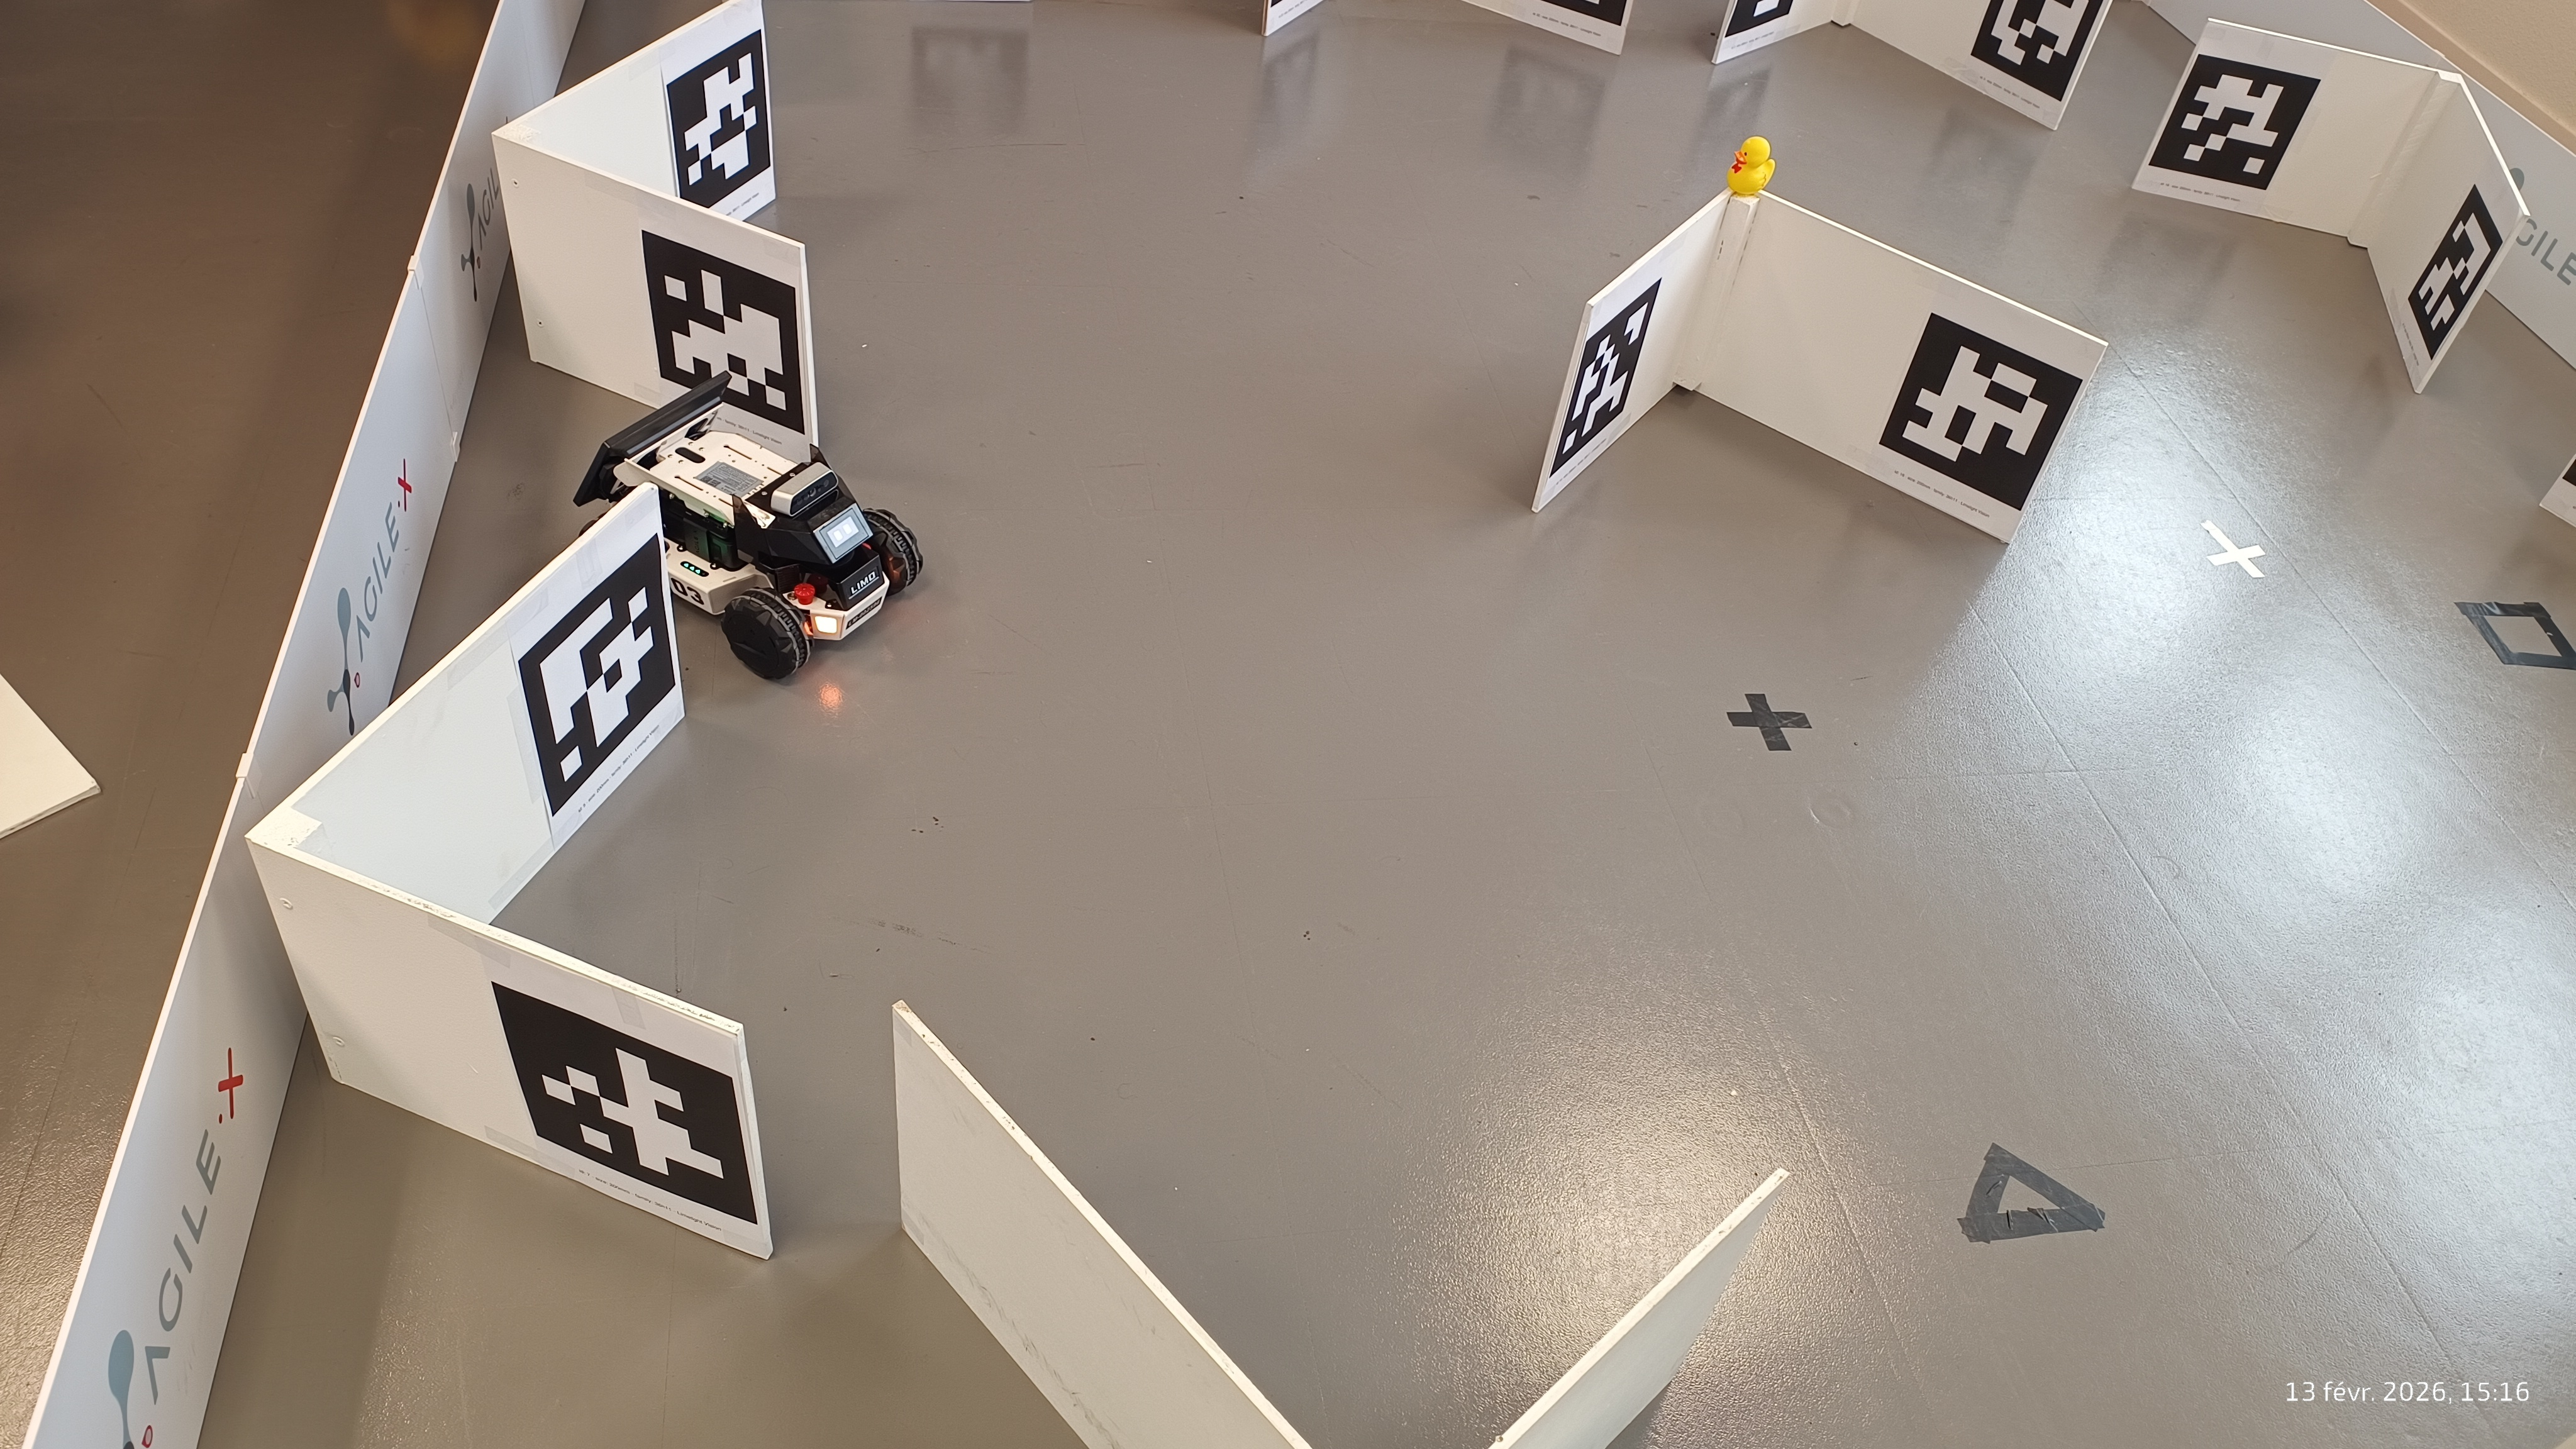
\includegraphics[width=3.35cm,height=3.30cm]{../assets/results/real_s1_reloc_015_foto.jpg}};
            \node[anchor=south west, inner sep=0pt] at (3.85,0.34)
              {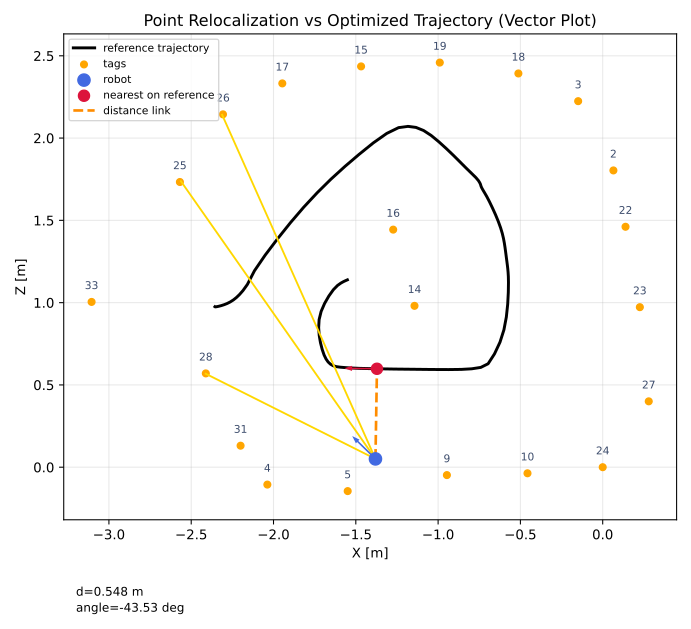
\includegraphics[width=3.35cm,height=3.30cm]{assets/results/graph_015.png}};
            \node[font=\scriptsize\bfseries, text=NavyBlue, anchor=north] at (1.98,0.30) {Point 015};
            \node[font=\scriptsize\bfseries, text=NavyBlue, anchor=north] at (5.53,0.30) {Graph 015};
          }
          % Pair 5: 016
          \only<6>{
            \node[anchor=south west, inner sep=0pt] at (0.30,0.34)
              {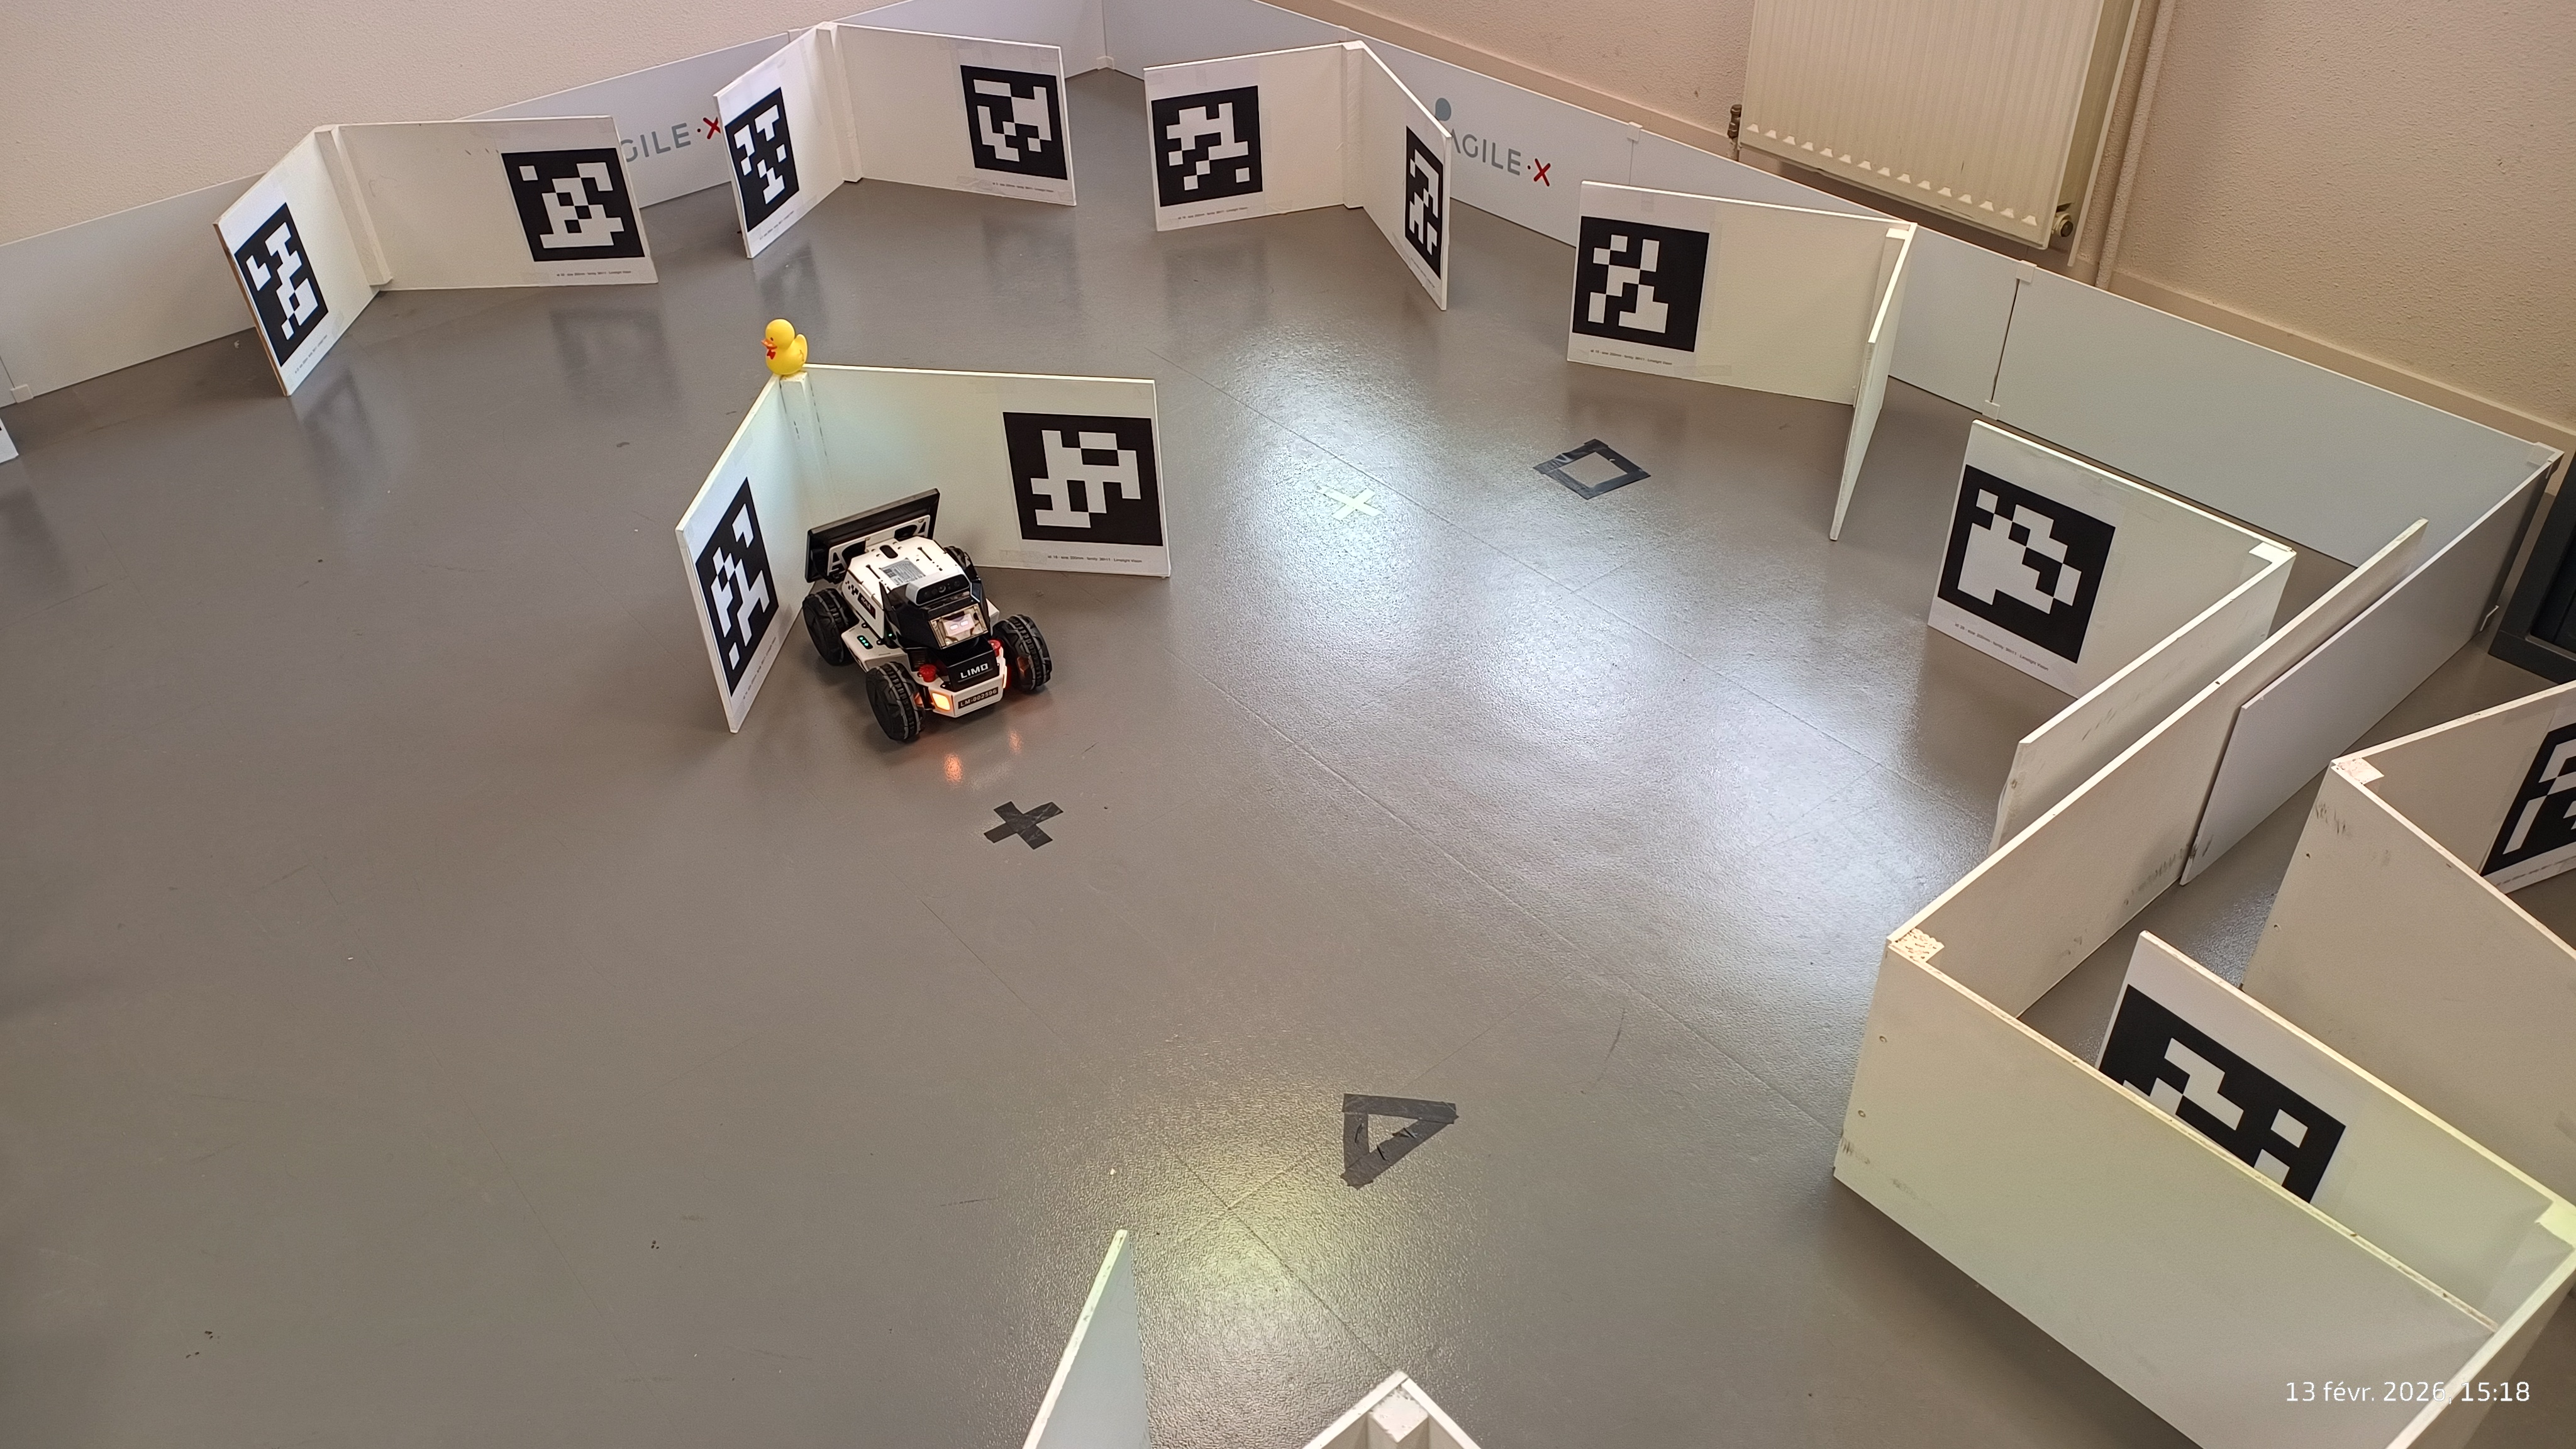
\includegraphics[width=3.35cm,height=3.30cm]{../assets/results/real_s1_reloc_016_foto.jpg}};
            \node[anchor=south west, inner sep=0pt] at (3.85,0.34)
              {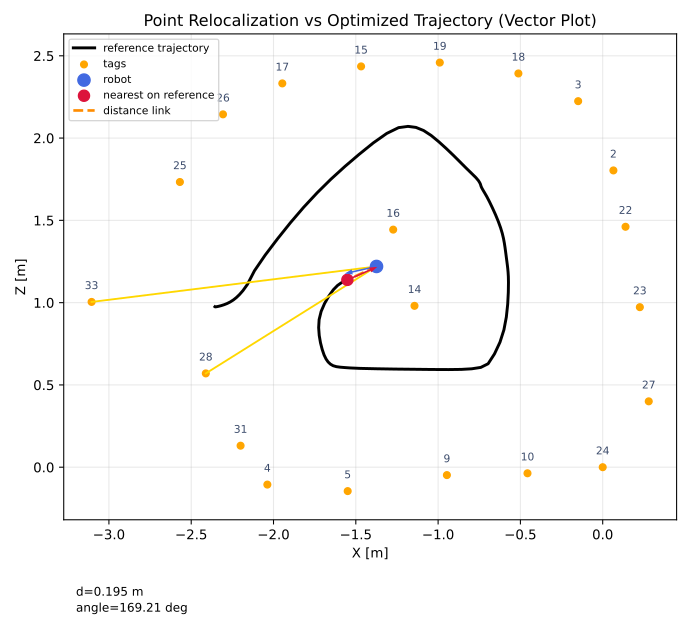
\includegraphics[width=3.35cm,height=3.30cm]{assets/results/graph_016.png}};
            \node[font=\scriptsize\bfseries, text=NavyBlue, anchor=north] at (1.98,0.30) {Point 016};
            \node[font=\scriptsize\bfseries, text=NavyBlue, anchor=north] at (5.53,0.30) {Graph 016};
          }
          % Pair 6: 018
          \only<7>{
            \node[anchor=south west, inner sep=0pt] at (0.30,0.34)
              {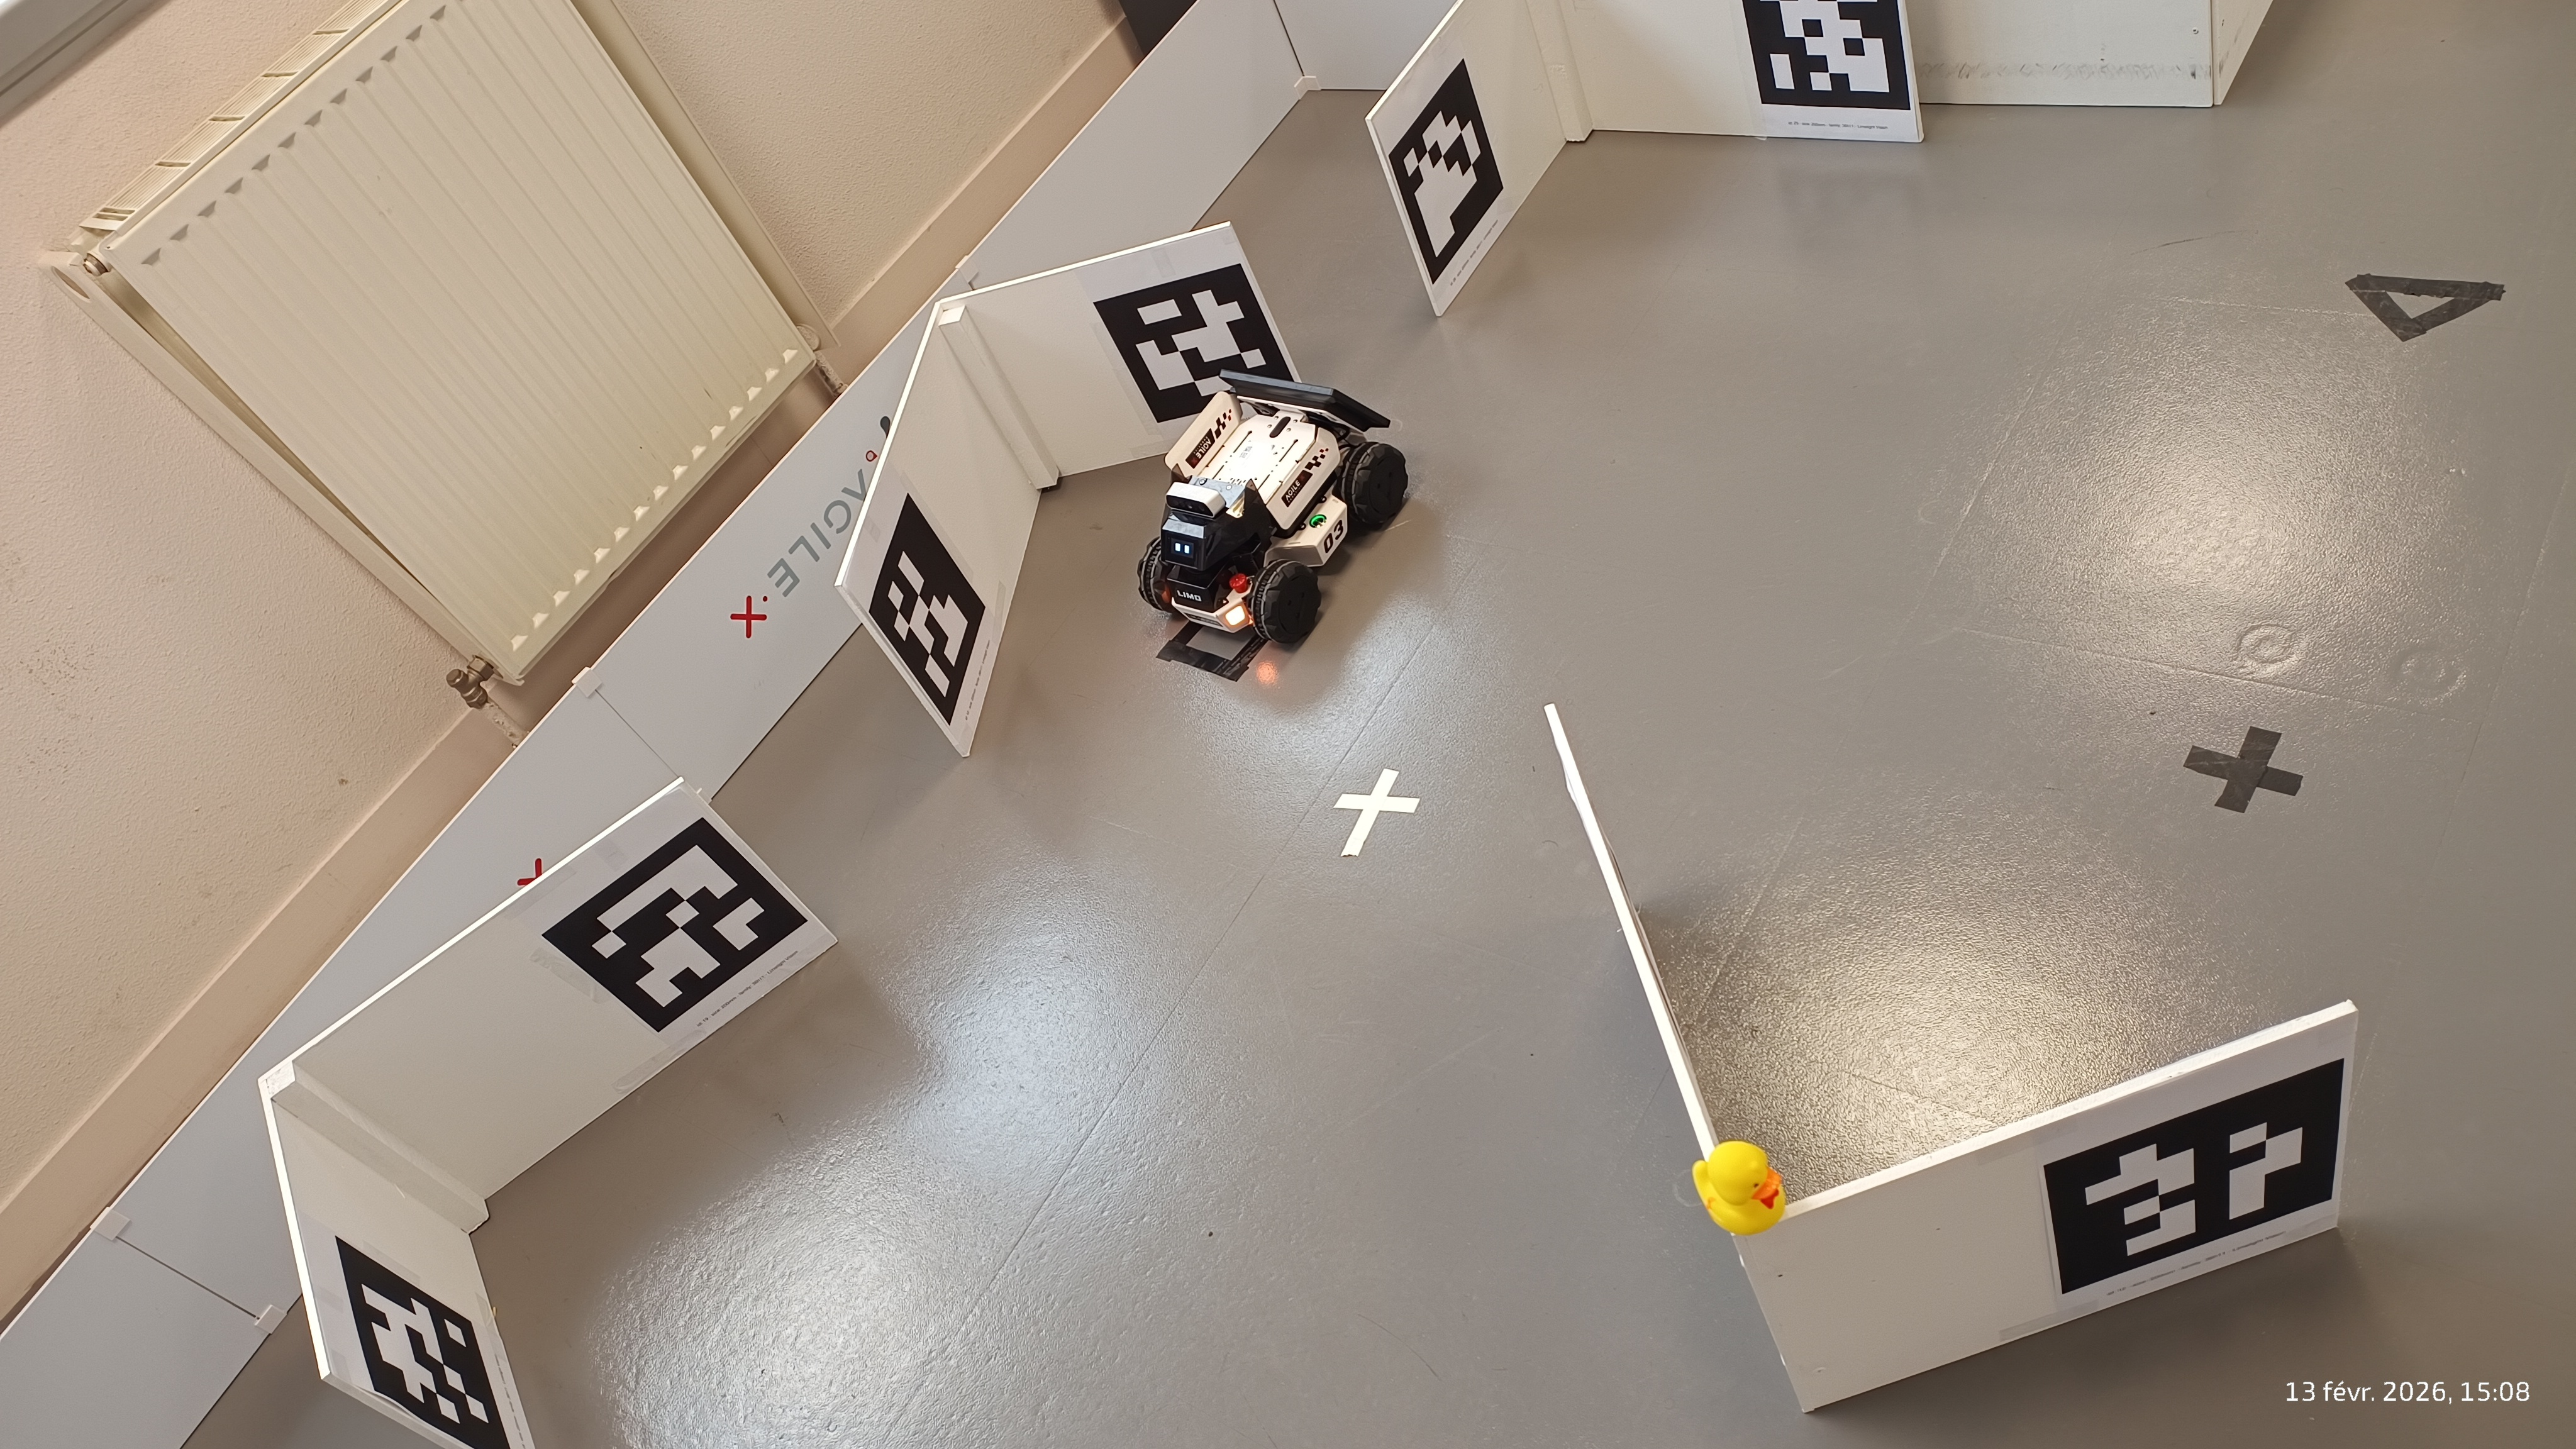
\includegraphics[width=3.35cm,height=3.30cm]{../assets/results/real_s1_reloc_018_foto.jpg}};
            \node[anchor=south west, inner sep=0pt] at (3.85,0.34)
              {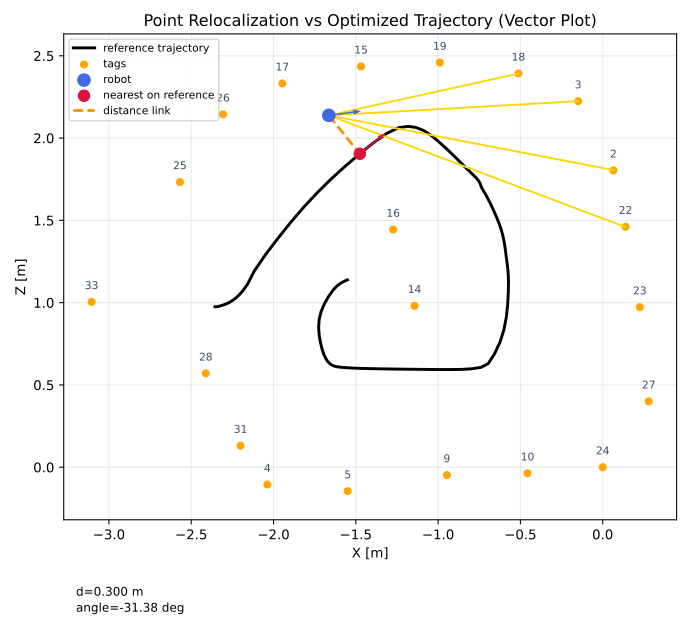
\includegraphics[width=3.35cm,height=3.30cm]{assets/results/graph_018.png}};
            \node[font=\scriptsize\bfseries, text=NavyBlue, anchor=north] at (1.98,0.30) {Point 018};
            \node[font=\scriptsize\bfseries, text=NavyBlue, anchor=north] at (5.53,0.30) {Graph 018};
          }
        \end{tikzpicture}
      }

      
    \end{outlinecard}
  \end{column}

  % ---------------- RIGHT: PIPELINE + EQUATIONS ----------------
  \begin{column}{0.35\textwidth}
    \begin{outlinecard}[Pipeline]
      \centering
      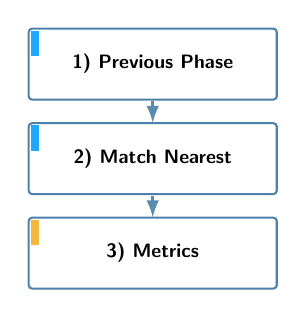
\begin{tikzpicture}[x=1cm,y=1cm,>=Latex]
        \node<1->[draw=NavyBlue!70, fill=white, rounded corners=1.2pt, line width=0.75pt,
          minimum width=3.15cm, minimum height=0.90cm, align=center] (p1) at (1.6,3.05)
          {\scriptsize\textbf{1) Previous Phase}};
        \node<2->[draw=NavyBlue!70, fill=white, rounded corners=1.2pt, line width=0.75pt,
          minimum width=3.15cm, minimum height=0.90cm, align=center] (p2) at (1.6,1.85)
          {\scriptsize\textbf{2) Match Nearest}};
        \node<3->[draw=NavyBlue!70, fill=white, rounded corners=1.2pt, line width=0.75pt,
          minimum width=3.15cm, minimum height=0.90cm, align=center] (p3) at (1.6,0.65)
          {\scriptsize\textbf{3) Metrics}};

        % active marker
        \fill<1>[AccentGold] ($(p1.north west)+(0.04,-0.04)$) rectangle ($(p1.north west)+(0.15,-0.36)$);
        \fill<2-6>[AccentGold] ($(p2.north west)+(0.04,-0.04)$) rectangle ($(p2.north west)+(0.15,-0.36)$);
        \fill<7->[AccentGold] ($(p3.north west)+(0.04,-0.04)$) rectangle ($(p3.north west)+(0.15,-0.36)$);

        % non-active marker
        \fill<2->[AccentBlue] ($(p1.north west)+(0.04,-0.04)$) rectangle ($(p1.north west)+(0.15,-0.36)$);
        \fill<7->[AccentBlue] ($(p2.north west)+(0.04,-0.04)$) rectangle ($(p2.north west)+(0.15,-0.36)$);

        \draw<2->[NavyBlue!65, line width=0.9pt, -{Latex[length=2.2mm,width=1.6mm]}] (1.6,2.58) -- (1.6,2.30);
        \draw<7->[NavyBlue!65, line width=0.9pt, -{Latex[length=2.2mm,width=1.6mm]}] (1.6,1.38) -- (1.6,1.10);
      \end{tikzpicture}
    \end{outlinecard}

    \vspace{-0.2cm}
    \only<1>{
      \begin{outlinecard}[From Previous Phase]
        \scriptsize
        
\begin{tikzpicture}[x=1cm,y=1cm]
          \node[anchor=west, text=NavyBlue, font=\scriptsize] at (0.00,0.78) {\faFile};
          \node[anchor=west, font=\scriptsize] at (0.35,0.78) {Reference trajectory};
          \node[anchor=west, font=\tiny\ttfamily] at (0.35,0.58) {trajetoria\_camera.csv};

          \node[anchor=west, text=NavyBlue, font=\scriptsize] at (0.00,0.36) {\faMapMarker};
          \node[anchor=west, font=\scriptsize] at (0.35,0.36) {Tag map};
          \node[anchor=west, font=\tiny\ttfamily] at (0.35,0.16) {tag\_map.yaml};
        \end{tikzpicture}
      \end{outlinecard}
    }

    \only<2-7>{
      \begin{outlinecard}[Nearest Projection]
        \scriptsize
        \[
          k^*=\arg\min_k \|\mathbf{p}_{\mathrm{cur}}-\mathbf{p}_k\|
        \]
        \[
          \mathbf{p}_{\mathrm{nearest}}=\mathbf{p}_{k^*}
        \]
      \end{outlinecard}
    }

    \only<7->{
      \begin{outlinecard}[Output Metrics]
        \scriptsize
        \[
          D=\|\mathbf{p}_{\mathrm{cur}}-\mathbf{p}_{\mathrm{nearest}}\|
        \]
        \[
          \phi=\mathrm{wrap}(\psi_{\mathrm{cur}}-\psi_{\mathrm{nearest}})
        \]
      \end{outlinecard}
     
    }
  \end{column}
\end{columns}

\end{frame}

\begin{frame}[label=slide-relocalization-demo]{Second Trajectory}
\vspace{-0.15cm}
\begin{center}
\begin{outlinecard}[Pipeline Running on Second Trajectory]
\centering
\begin{tikzpicture}[x=1cm,y=1cm]
  % Embedded video (annex style, with fallback)
  \node[inner sep=0pt, anchor=south west] at (0.45,0.55)
    {%
      \IfFileExists{assets/Reloc_scnerio2_2x.mp4}{%
        \movie[
          width=11.10cm,
          height=5.10cm,
          poster
        ]{%
          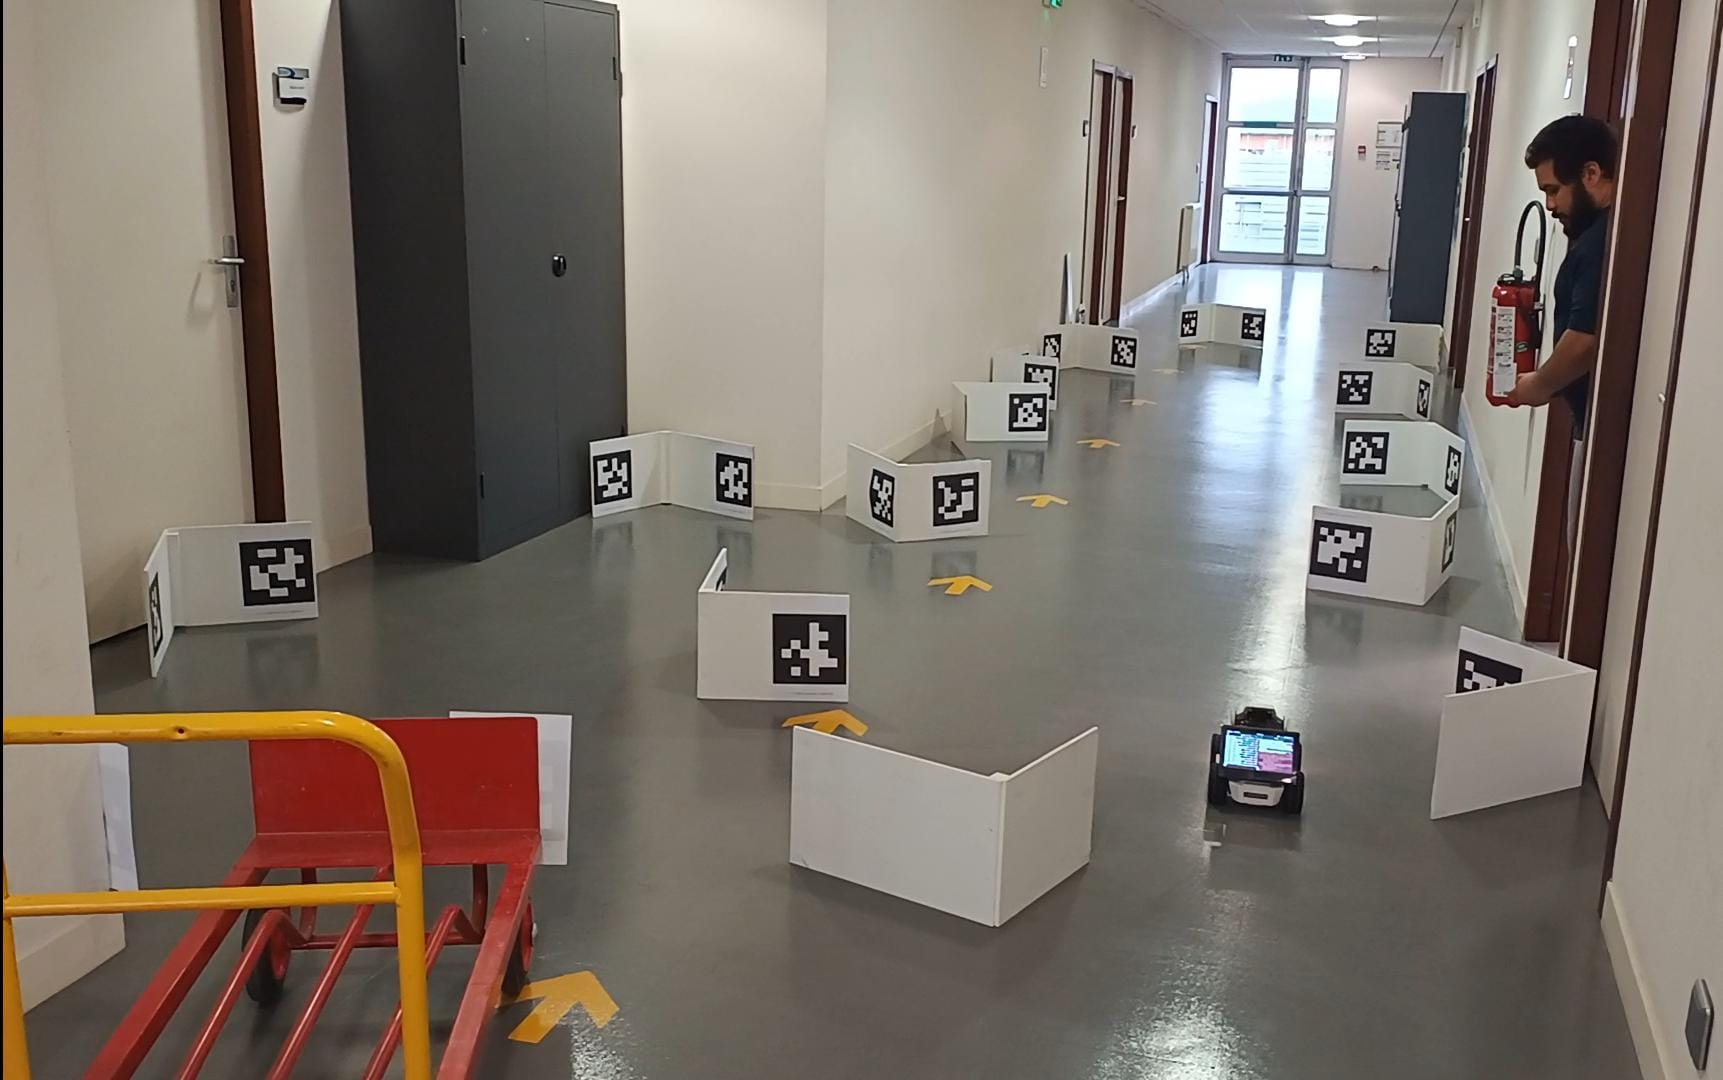
\includegraphics[
            width=11.10cm,
            height=5.10cm
          ]{assets/scneario2.jpeg}%
        }{assets/Reloc_scnerio2_2x.mp4}%
      }{%
        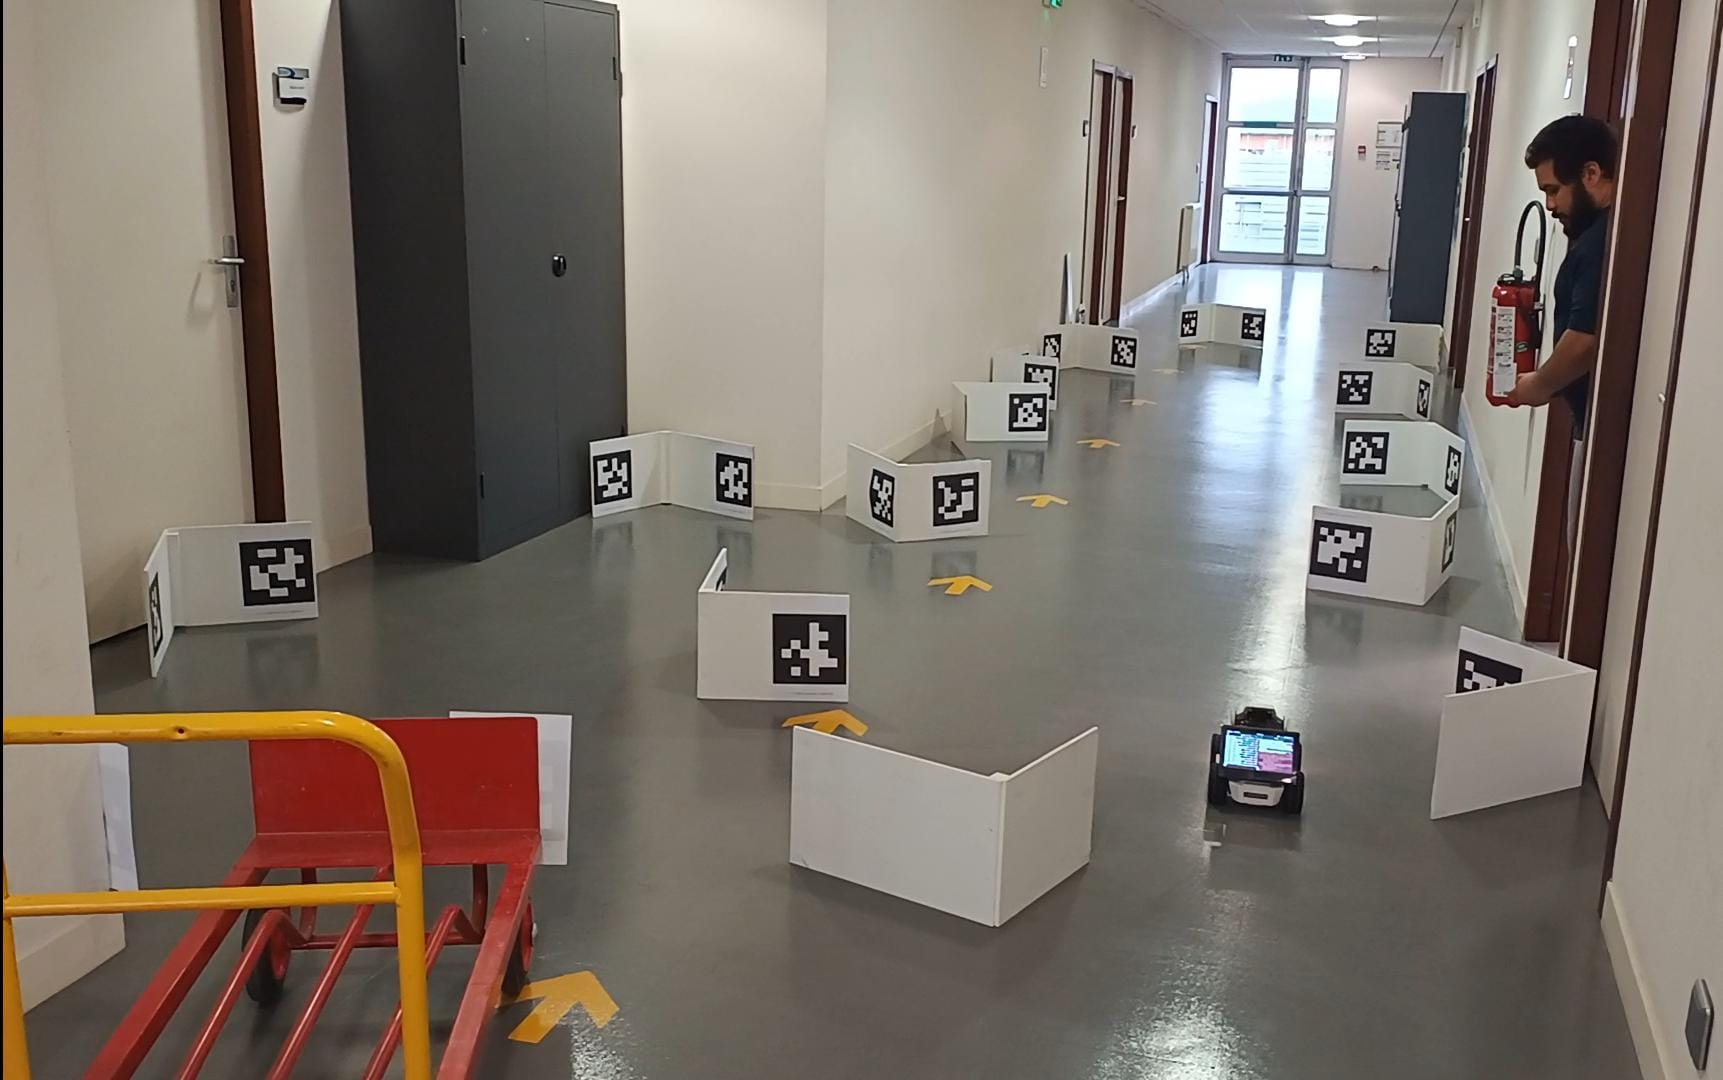
\includegraphics[width=11.10cm,height=5.10cm]{assets/scneario2.jpeg}%
      }%
    };

  \fill[black, opacity=0.16] (0.45,0.55) rectangle (11.55,5.65);
  \fill[white, opacity=0.95] (6.00,3.10) circle (0.35);
  \fill[NavyBlue] (5.88,2.95) -- (5.88,3.25) -- (6.16,3.10) -- cycle;

\end{tikzpicture}
\end{outlinecard}
\end{center}
\end{frame}

\begin{frame}[label=slide-conclusion]{Conclusion}
% Template only — Discussion and Conclusion
\vspace{0.2cm}
\begin{outlinecard}[Discussion and Conclusion — Template]
\small
\textbf{To fill later:}
\begin{itemize}
  \item Main findings
  \item Current limitations
  \item Scope boundaries
  \item Next steps
\end{itemize}
\end{outlinecard}

\end{frame}

\begin{frame}{References}
	\transfade[duration=0.25]
	\scriptsize
	\setbeamertemplate{bibliography item}{\insertbiblabel}
	\begin{thebibliography}{9}
		\bibitem{github}
		Project Repository,
		\textit{Record, Map, and Relocalize with AprilTags (ROS 2)},
		GitHub. Available at: \url{https://github.com/Wirelessbrains/project_record_relocalize_apriltags_M2_PAR
		}.
		
		\bibitem{report}
		J. P. M. do Lago Reis and Y. K. da Silva Ramos,
		\textit{An AprilTag-Based Approach to Trajectory
			Recording and Relocalization for Mobile Robots},
		M2 PAR Project Report, 2026.
		
		\bibitem{wang2016iros}
		J. Wang and E. Olson,
		\textit{AprilTag 2: Efficient and robust fiducial detection},
		IEEE/RSJ IROS, 2016.
		
		\bibitem{Fischler1981}
		M. A. Fischler and R. C. Bolles,
		\textit{Random Sample Consensus: A Paradigm for Model Fitting with Applications to Image Analysis and Automated Cartography},
		Communications of the ACM, 1981.
		
		\bibitem{triggs1999ba}
		B. Triggs, P. McLauchlan, R. Hartley, and A. Fitzgibbon,
		\textit{Bundle Adjustment: A Modern Synthesis},
		Vision Algorithms Workshop, 1999.
	\end{thebibliography}
	\setbeamertemplate{bibliography item}[book]
\end{frame}


% ==================/// END PRESENTATION
% ==================///==================///==================///

\begin{frame}[plain]
	
	% Logos no canto superior direito (como nos outros slides)
	\begin{tikzpicture}[remember picture,overlay]
		\node[anchor=north east] 
		at ($(current page.north east)+(-0.8cm,-0.6cm)$) {
			
\includegraphics[height=1.0cm]{assets/logo_UCA.jpg}

		};
	\end{tikzpicture}
	
	\centering
	\vspace*{2.2cm}
	
	{\Huge\bfseries\textcolor{NavyBlue}{Thank you for listening!}\par}
	\vspace{0.4cm}
	{\Large\textcolor{CoolGray}{Any questions?}\par}
	
	\vspace{0.9cm}
	{\color{AccentBlue}\rule{3cm}{1.5pt}\par}
	
	\vspace{0.7cm}
	{\small\textcolor{CoolGray}{ Joao Pedro Martins do Lago Reis \quad|\quad Yann Kelvem da Silva Ramos}\par}
	{\small\textcolor{CoolGray}{Record, Map, and Relocalize with AprilTags}\par}
	
\end{frame}


\appendix
\begin{frame}[noframenumbering]{Appendix Summary}
\transfade[duration=0.25]
\begin{outlinecard}[Click a Title to Open the Appendix Slide]
  \tiny
  \begin{columns}[T,onlytextwidth]
    \begin{column}{0.5\textwidth}
      \begin{itemize}
        \item \hyperlink{appendix-project-links}{\textbf{Appendix - Project Links (QR Codes)}}
        \item \hyperlink{appendix-recording-setup}{\textbf{Appendix - Recording Simulation Setup}}
        \item \hyperlink{appendix-synth-noisefree}{\textbf{Appendix - Noise-Free Optimized Reconstruction}}
        \item \hyperlink{appendix-synth-noisy}{\textbf{Appendix - Noisy Optimized Reconstruction (+10 cm)}}
        \item \hyperlink{appendix-mosaic-architecture}{\textbf{Appendix - Evaluation Environments (Real and Simulated)}}
        \item \hyperlink{appendix-mosaic-detection}{\textbf{Appendix - AprilTag Detection Samples}}
        \item \hyperlink{appendix-mosaic-rec-traj}{\textbf{Appendix - Reconstructed Trajectory}}
        \item \hyperlink{appendix-mosaic-compare-gt}{\textbf{Appendix - Optimized vs Ground Truth}}
        \item \hyperlink{appendix-mosaic-synth-points}{\textbf{Appendix - Synthetic YZ Relocalization Points}}
        \item \hyperlink{appendix-mosaic-real-recording}{\textbf{Appendix - Real Recording Result}}
      \end{itemize}
    \end{column}
    \begin{column}{0.5\textwidth}
      \begin{itemize}
        \item \hyperlink{appendix-mosaic-real-relocal}{\textbf{Appendix - Real Relocalization Validation}}
        \item \hyperlink{appendix-mosaic-second-recording}{\textbf{Appendix - Second Real Recording Result}}
        \item \hyperlink{appendix-discussion-recording-limitations}{\textbf{Appendix - Recording Limitations}}
        \item \hyperlink{appendix-flowchart-recording}{\textbf{Appendix - Offline Recording Flowchart}}
        \item \hyperlink{appendix-flowchart-relocal}{\textbf{Appendix - Relocalization Flowchart}}
        \item \hyperlink{appendix-design-apriltag-family}{\textbf{Appendix - Why AprilTag tag36h11}}
        \item \hyperlink{appendix-design-heading-anchor}{\textbf{Appendix - Why Heading Deviation and Anchoring}}
        \item \hyperlink{appendix-design-estimation-stack}{\textbf{Appendix - Why PnP + Graph + Procrustes}}
        \item \hyperlink{appendix-table-20}{\textbf{Appendix - Table 2.0 (Functional Requirements)}}
        \item \hyperlink{appendix-table-21}{\textbf{Appendix - Table 2.1 (Non-Functional Requirements)}}
        \item \hyperlink{appendix-table-22}{\textbf{Appendix - Table 2.2 (Deliverables and Constraints)}}
        \item \hyperlink{appendix-table-23}{\textbf{Appendix - Table 2.3 (Technical Limitations)}}
        \item \hyperlink{appendix-table-41}{\textbf{Appendix - Table 4.1 (Residual Errors, No Noise)}}
        \item \hyperlink{appendix-table-42}{\textbf{Appendix - Table 4.2 (Errors, +10 cm Noise)}}
        \item \hyperlink{appendix-table-43}{\textbf{Appendix - Table 4.3 (Estimated vs Measured $D,\phi$)}}
        \item \hyperlink{appendix-table-a1}{\textbf{Appendix - Table A.1 (Tag 16 Distance Comparison)}}
      \end{itemize}
    \end{column}
  \end{columns}
\end{outlinecard}
\end{frame}
\begin{frame}[noframenumbering]{Appendix Summary}
\transfade[duration=0.25]
\begin{outlinecard}[Appendix Media]
  \tiny
  \begin{itemize}
    \item \hyperlink{appendix-media-validation-exp2}{\textbf{Appendix - Media: Validation Experiment 2}}
    \item \hyperlink{appendix-media-reloc-demo1}{\textbf{Appendix - Media: Relocalization Demo 1}}
    \item \hyperlink{appendix-media-reloc-demo2}{\textbf{Appendix - Media: Relocalization Demo 2}}
    \item \hyperlink{appendix-media-reloc-real1}{\textbf{Appendix - Media: Real Relocalization Scenario 1}}
    \item \hyperlink{appendix-media-reloc-scn2}{\textbf{Appendix - Media: Real Relocalization Scenario 2}}
    \item \hyperlink{appendix-media-control-law}{\textbf{Appendix - Media: Control-Law Parking Experiment}}
    \item \hyperlink{appendix-media-traj1}{\textbf{Appendix - Media: Trajectory Playback}}
  \end{itemize}
\end{outlinecard}
\end{frame}
\startappendixframes
\begin{frame}[label=appendix-recording-setup]{Appendix - Recording Simulation Setup}
\transfade[duration=0.25]
\vspace{-0.08cm}
\begin{outlinecard}[Simulation Environment]
  \begin{columns}[T,onlytextwidth]
    \begin{column}{0.5\textwidth}
      \centering
      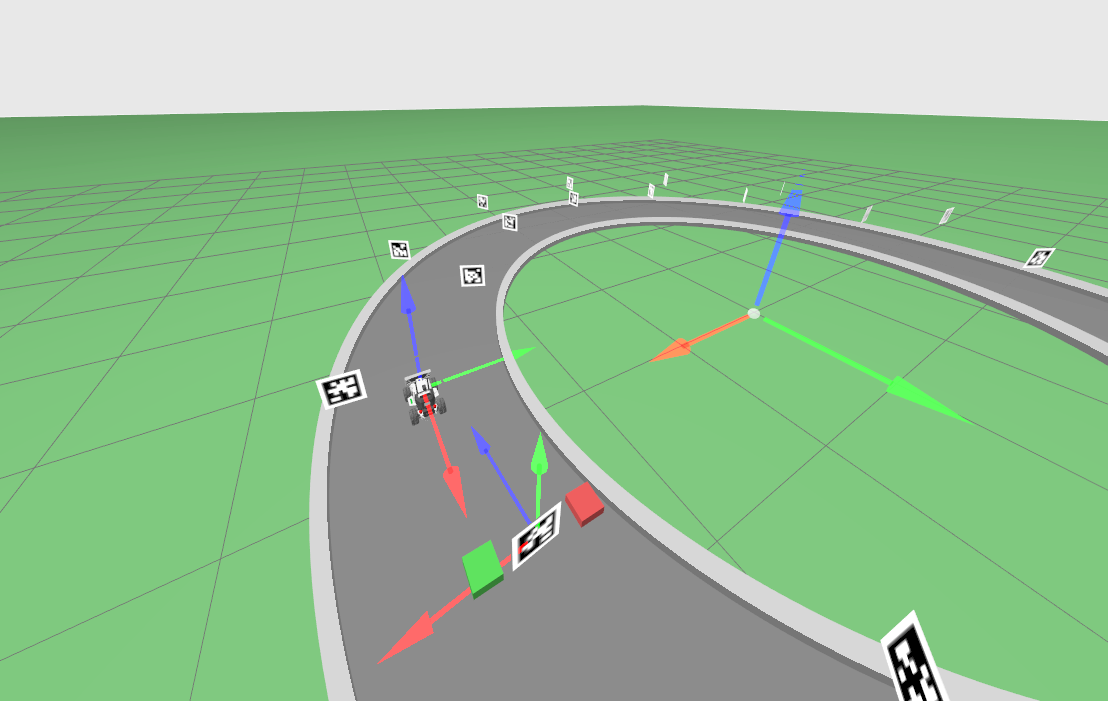
\includegraphics[width=0.96\linewidth,height=0.30\textheight,keepaspectratio]{../Report/Images/limo_simulation_environment.png}\\[-0.5mm]
      {\tiny Gazebo scenario with fixed AprilTags}
    \end{column}
    \begin{column}{0.5\textwidth}
      \centering
      \only<3->{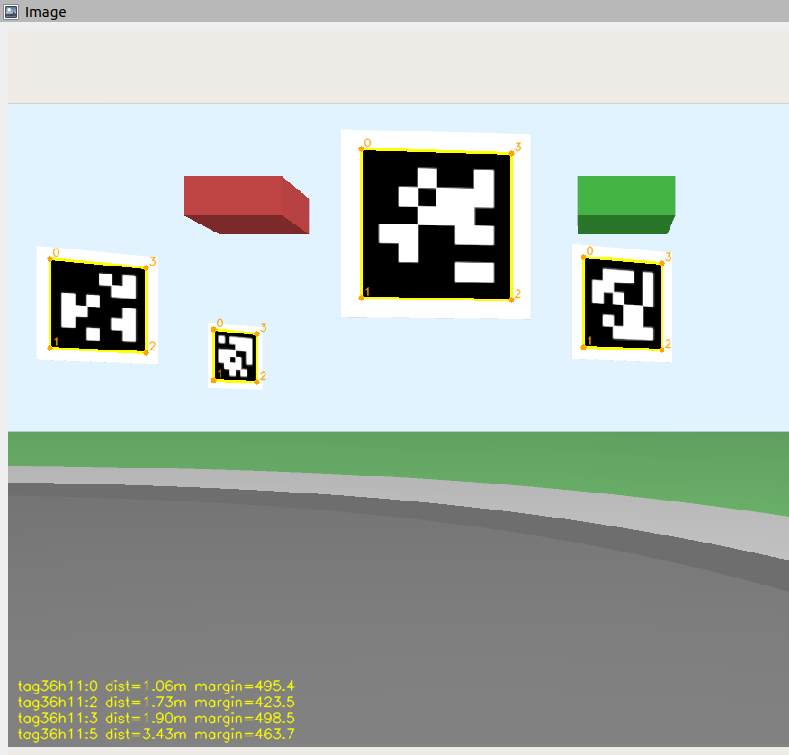
\includegraphics[width=0.96\linewidth,height=0.30\textheight,keepaspectratio]{../Report/Images/apriltag_detection_sim.png}\\[-0.5mm]}
      \only<3->{\tiny Simulated AprilTag detection input}
    \end{column}
  \end{columns}
\end{outlinecard}

\vspace{-0.05cm}
\begin{outlinecard}[Recording Inputs]
  \scriptsize
  \begin{itemize}
    \item<1-> Initial traversal logged into \texttt{rosbag2}.
    \item<2-> Camera intrinsics and AprilTag detections are stored frame-by-frame.
    \item<3-> This dataset feeds the offline map-and-trajectory reconstruction.
  \end{itemize}
\end{outlinecard}
\end{frame}

\edef\SimulationVideoFile{\detokenize{assets/simulation_validation.mp4}}
\edef\SimulationPosterFile{\detokenize{assets/simulation_validation_thumb.jpg}}
\edef\SimulationGraphPdfFile{\detokenize{../Report/svg-inkscape/sim_perception_gt_01_outputs_global_stride2__recording_trajectory_with_detected_and_groundtruth_tags_svg-raw.pdf}}
\colorlet{ValidationFrameColor}{NavyBlue}


\begin{frame}[label=appendix-synth-noisefree]{Optimized tag map and reconstructed camera trajectory in the noise-free scenario.}
\vspace{-0.08cm}
\centering
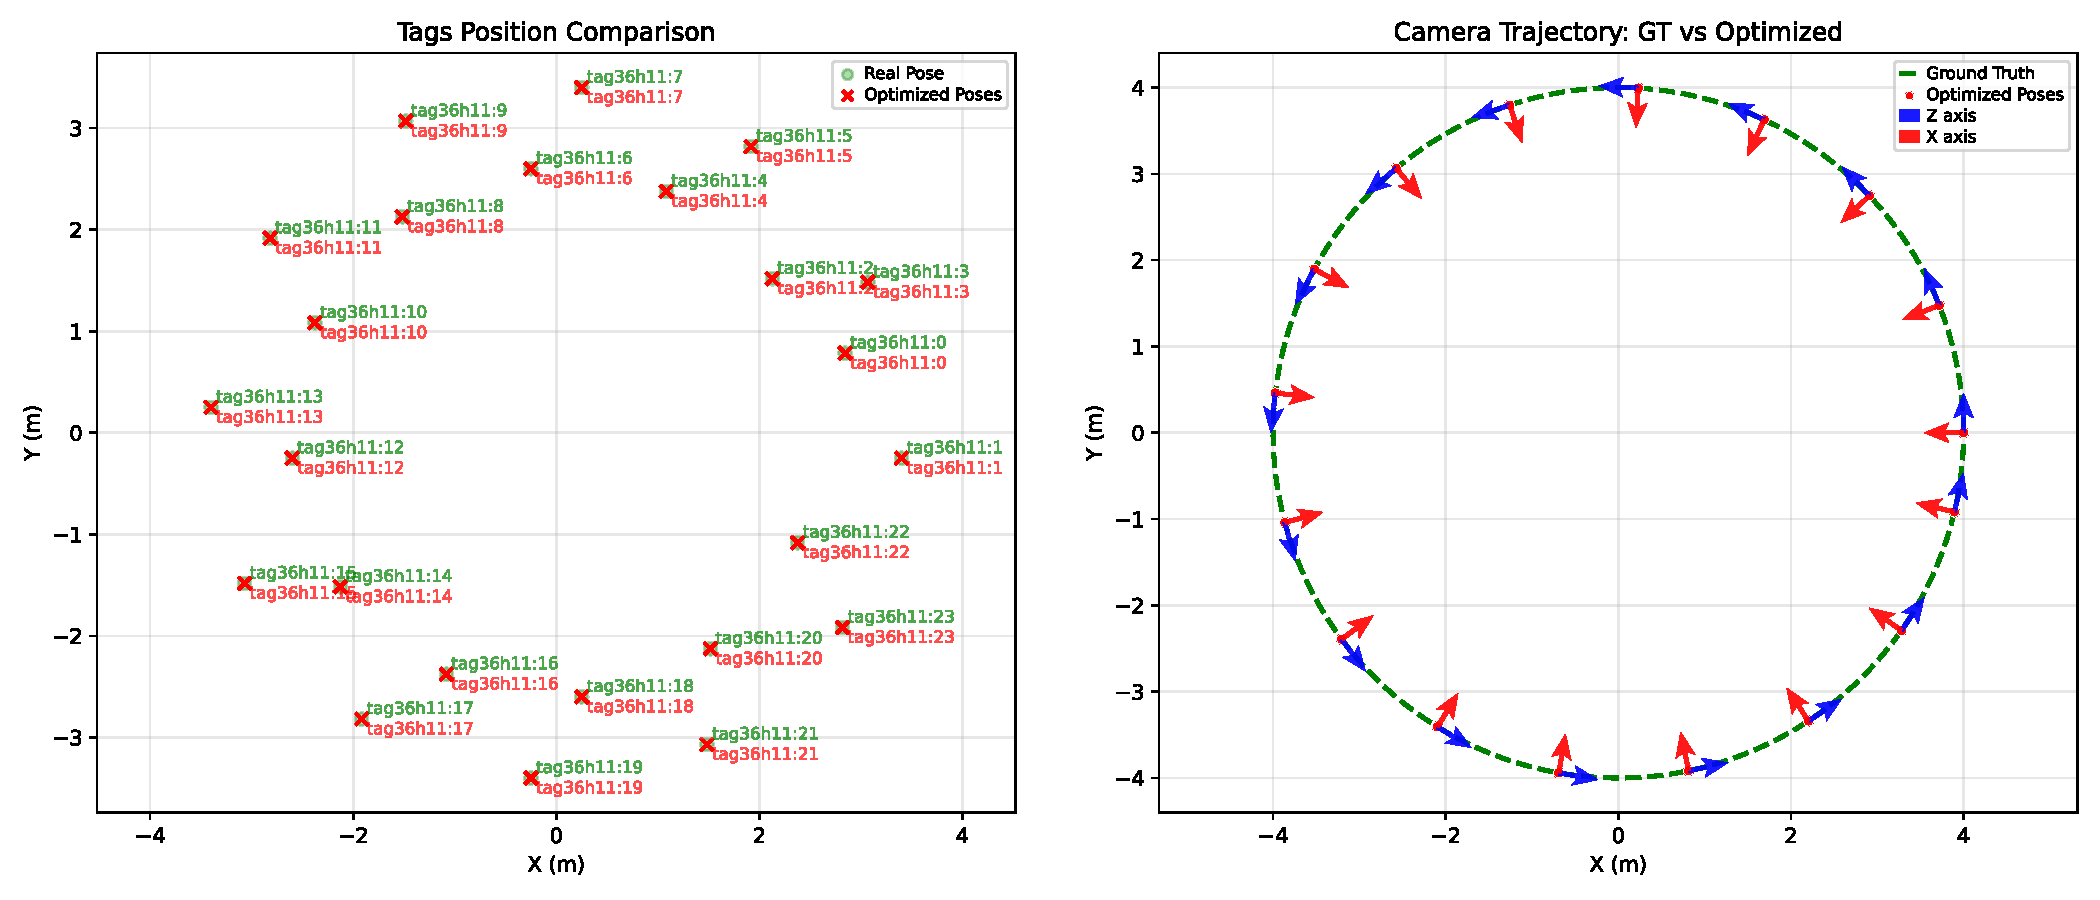
\includegraphics[width=0.92\linewidth,height=0.72\textheight,keepaspectratio]{../Report/svg-inkscape/comparison_optimized_lm_svg-raw.pdf}
\end{frame}

\begin{frame}[label=appendix-synth-noisy]{Optimized tag map and reconstructed trajectory under 10 cm Gaussian noise.}
\vspace{-0.08cm}
\centering
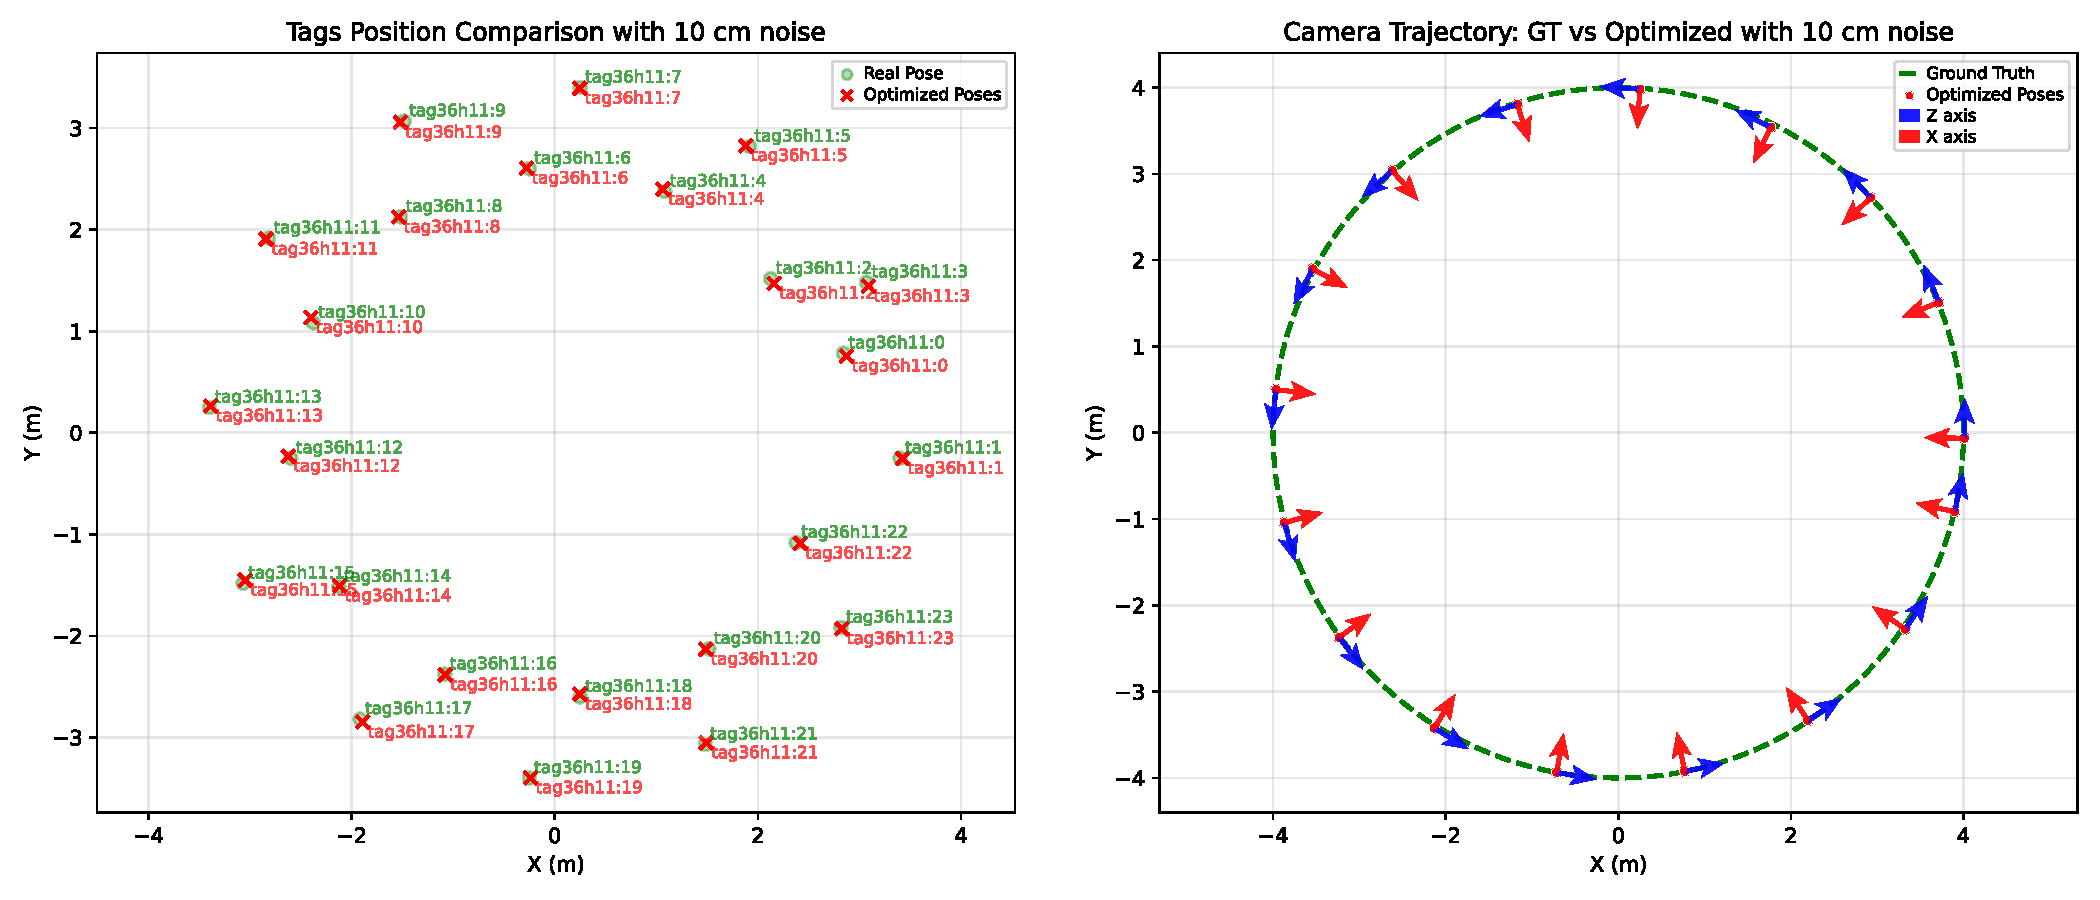
\includegraphics[width=0.92\linewidth,height=0.72\textheight,keepaspectratio]{../Report/svg-inkscape/comparison_optimized_lm_noise_10cm_svg-raw.pdf}
\end{frame}

\begin{frame}[label=appendix-mosaic-architecture]{Physical and simulated setups used to evaluate the proposed architecture.}
  \begin{columns}[c,onlytextwidth]
    \begin{column}{0.49\textwidth}
      \centering
      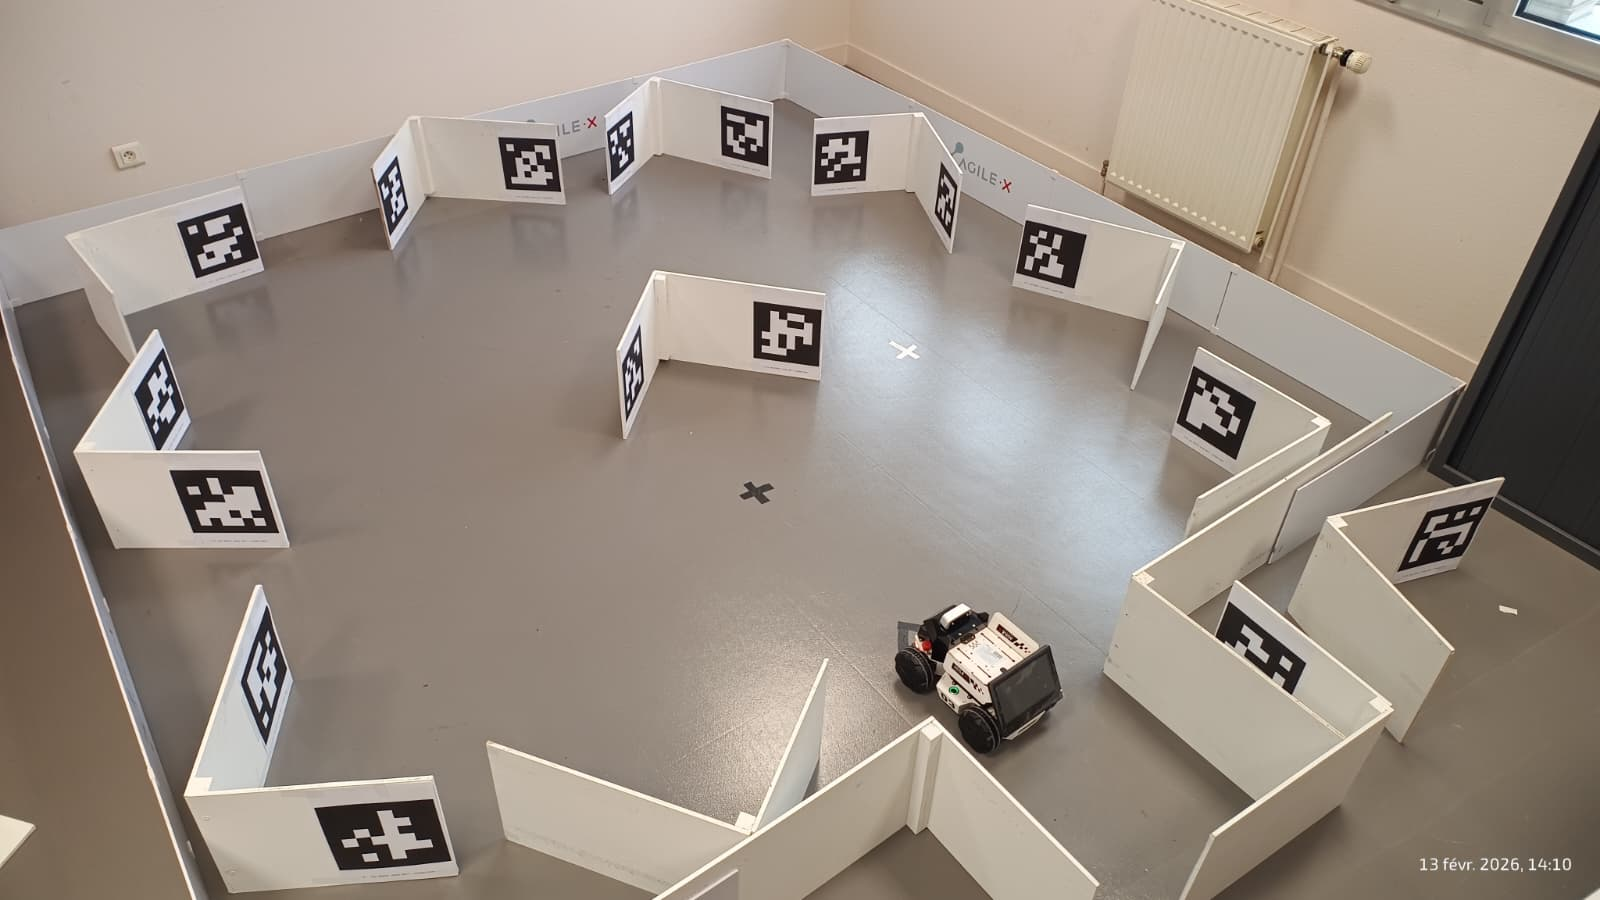
\includegraphics[width=\linewidth,height=0.65\textheight,keepaspectratio]{../Report/Images/limo_real_environment.png}
    \end{column}
    \begin{column}{0.49\textwidth}
      \centering
      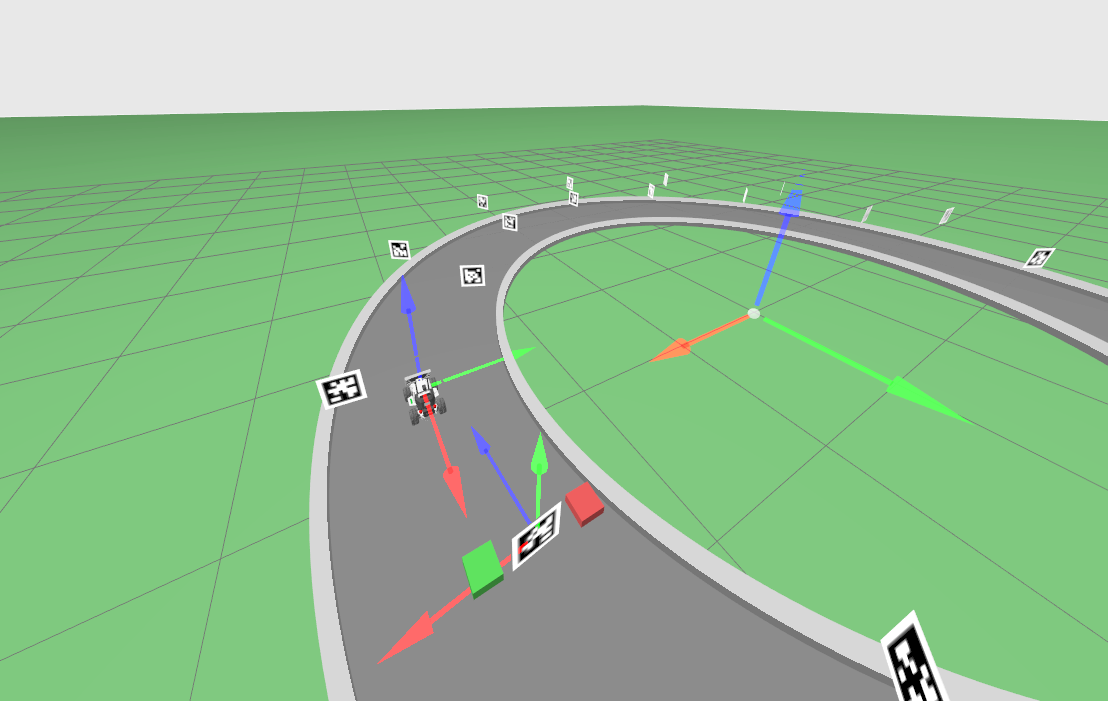
\includegraphics[width=\linewidth,height=0.65\textheight,keepaspectratio]{../Report/Images/limo_simulation_environment.png}
    \end{column}
  \end{columns}
\end{frame}

\begin{frame}[label=appendix-mosaic-detection]{Representative detection, each detected tag yields a camera-relative pose estimate obtained through a PnP formulation.}
  \begin{columns}[c,onlytextwidth]
    \begin{column}{0.49\textwidth}
      \centering
      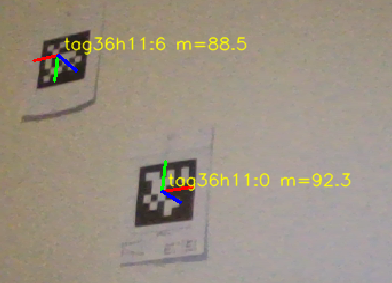
\includegraphics[width=0.96\linewidth,height=0.58\textheight,keepaspectratio]{../Report/Images/apriltag_detection_real.png}
    \end{column}
    \begin{column}{0.49\textwidth}
      \centering
      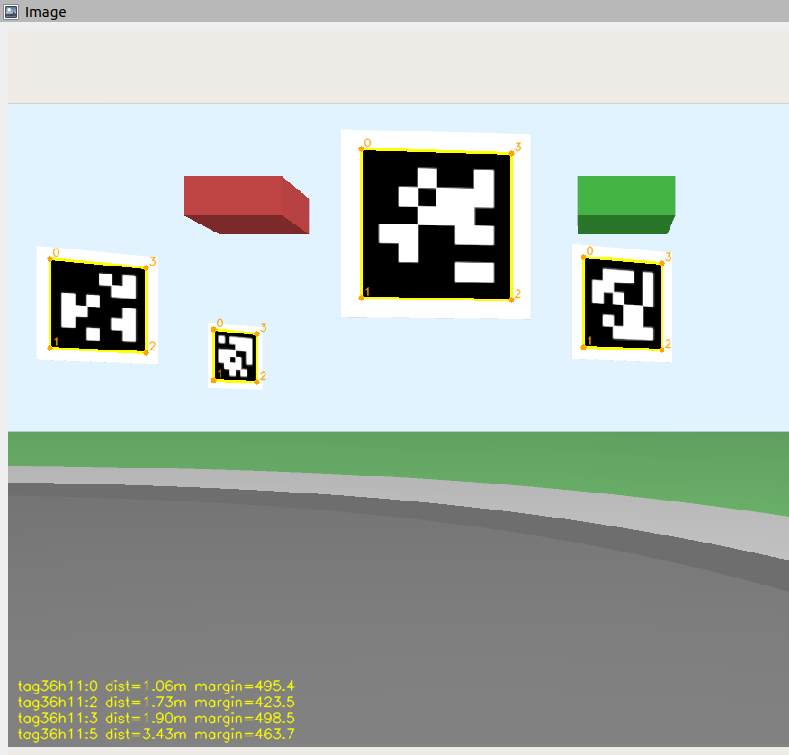
\includegraphics[width=0.96\linewidth,height=0.58\textheight,keepaspectratio]{../Report/Images/apriltag_detection_sim.png}
    \end{column}
  \end{columns}
\end{frame}

\begin{frame}[label=appendix-mosaic-rec-traj]{Reconstructed camera trajectory obtained after map optimization.}
  \begin{columns}[c,onlytextwidth]
    \begin{column}{0.49\textwidth}
      \centering
      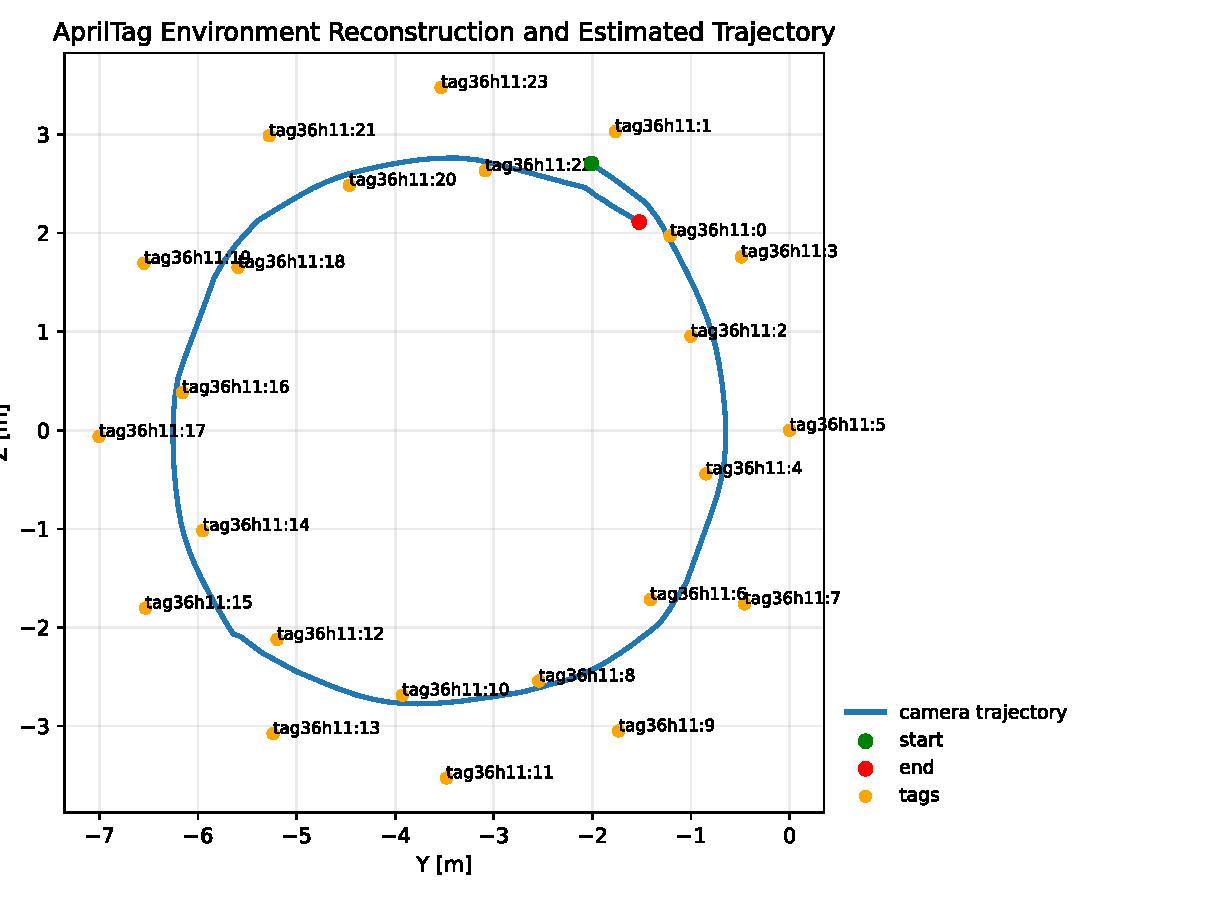
\includegraphics[width=\linewidth,height=0.65\textheight,keepaspectratio]{../Report/svg-inkscape/sim_perception_gt_01_outputs_global_stride2__recording_trajectory_basic_svg-raw.pdf}
    \end{column}
    \begin{column}{0.49\textwidth}
      \centering
      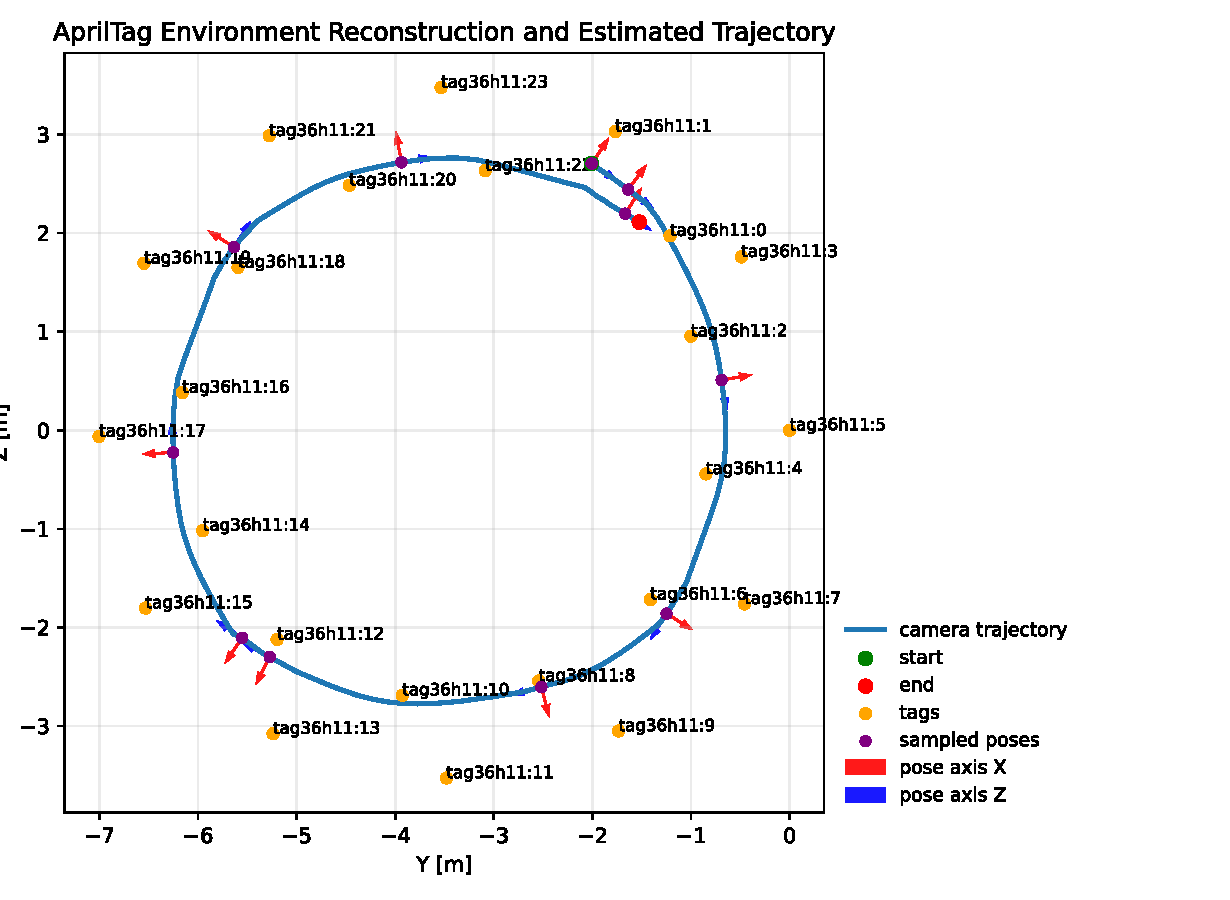
\includegraphics[width=\linewidth,height=0.65\textheight,keepaspectratio]{../Report/svg-inkscape/sim_perception_gt_01_outputs_global_stride2__recording_trajectory_with_axes_svg-raw.pdf}
    \end{column}
  \end{columns}
\end{frame}

\begin{frame}[label=appendix-mosaic-compare-gt]{Comparison between optimized reconstruction and ground-truth configuration.}
  \begin{columns}[c,onlytextwidth]
    \begin{column}{0.49\textwidth}
      \centering
      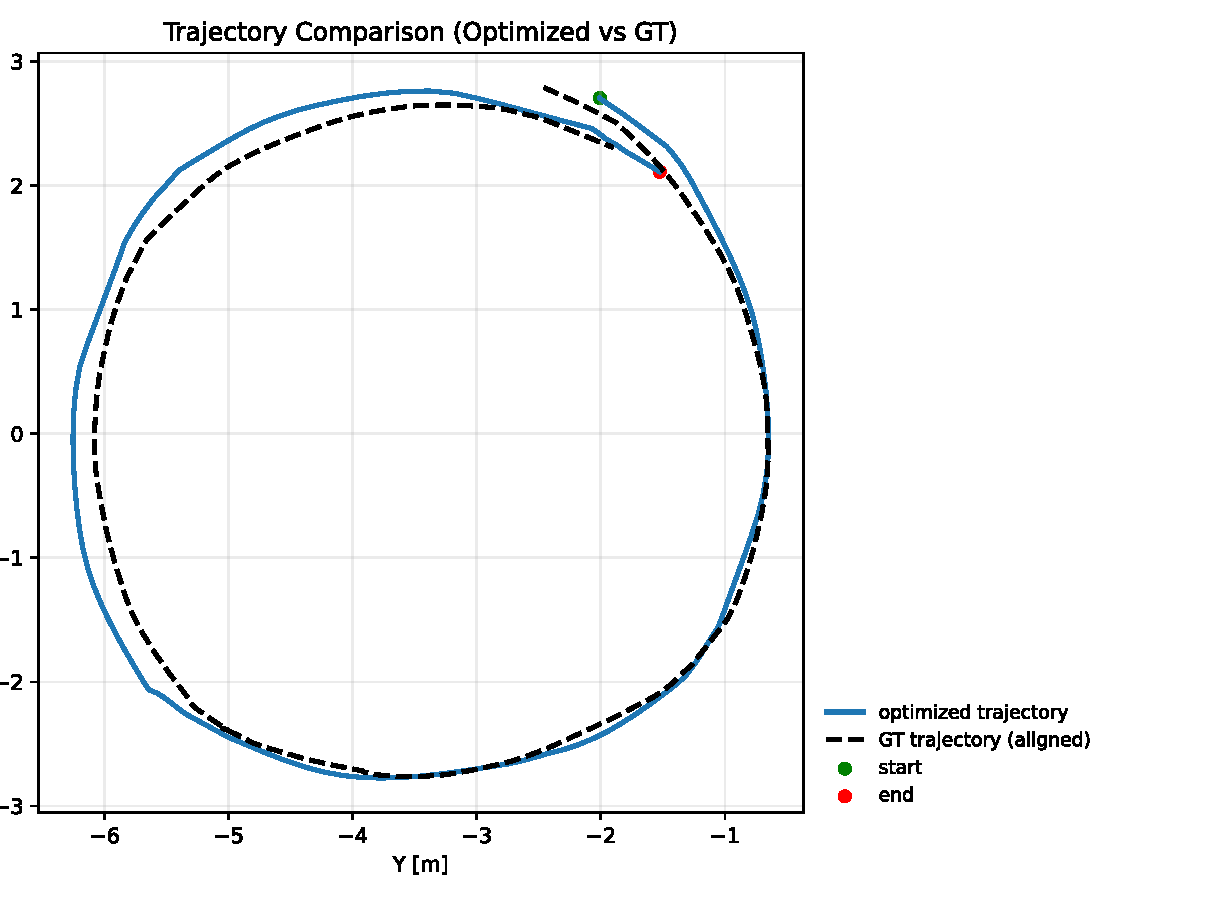
\includegraphics[width=\linewidth,height=0.65\textheight,keepaspectratio]{../Report/svg-inkscape/sim_perception_gt_01_outputs_global_stride2__recording_trajectory_comparison_optimized_vs_gt_svg-raw.pdf}
    \end{column}
    \begin{column}{0.49\textwidth}
      \centering
      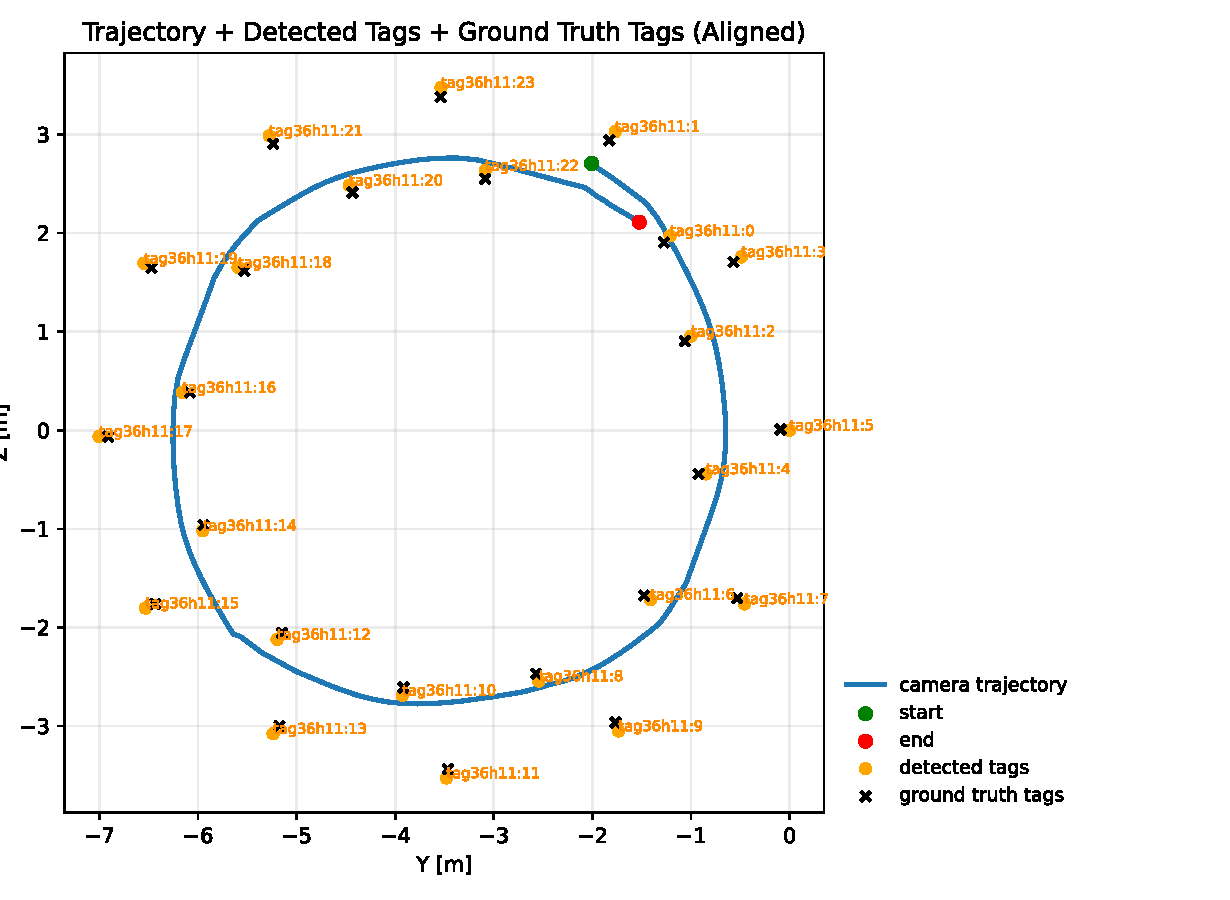
\includegraphics[width=\linewidth,height=0.65\textheight,keepaspectratio]{../Report/svg-inkscape/sim_perception_gt_01_outputs_global_stride2__recording_trajectory_with_detected_and_groundtruth_tags_svg-raw.pdf}
    \end{column}
  \end{columns}
\end{frame}

\begin{frame}[label=appendix-mosaic-synth-points]{Representative synthetic points used to validate the computation of $D$ in the YZ plane.}
  \begin{columns}[c,onlytextwidth]
    \begin{column}{0.49\textwidth}
      \centering
      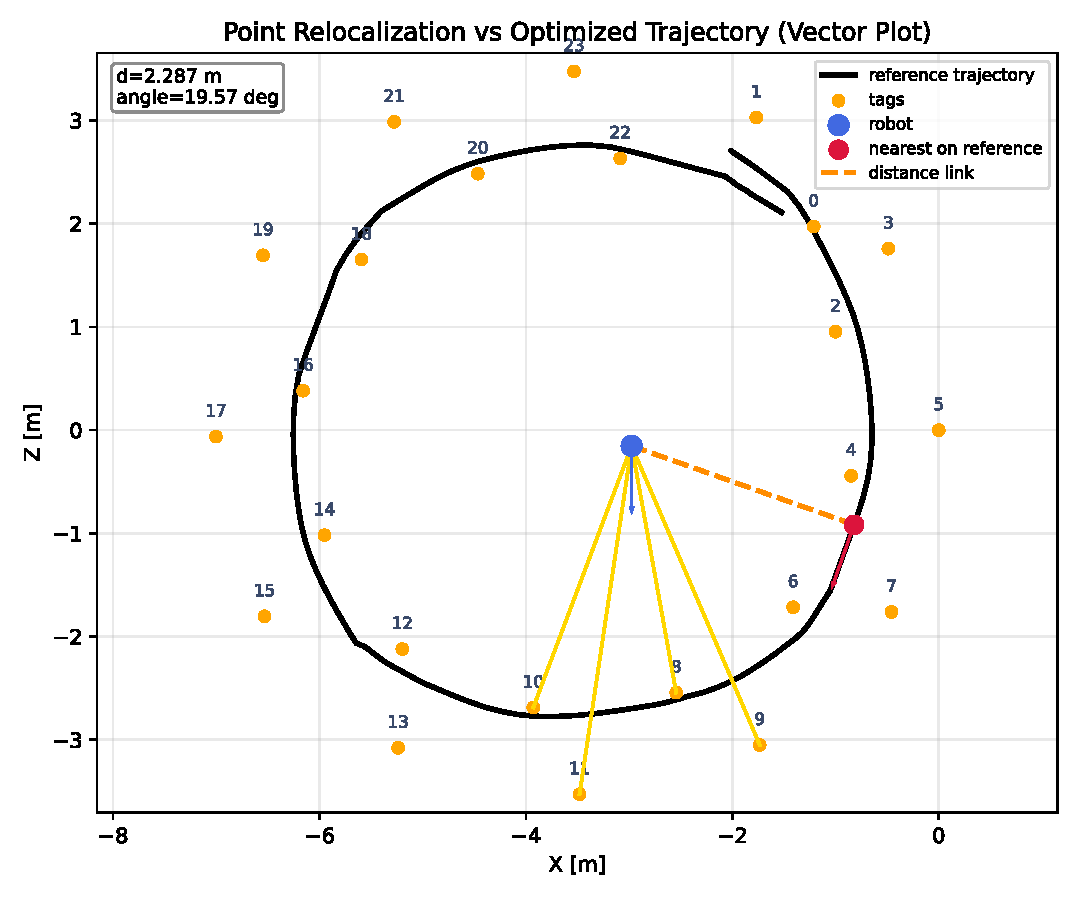
\includegraphics[width=\linewidth,height=0.65\textheight,keepaspectratio]{../Report/svg-inkscape/output_sim_between_tags_yz_01__relocalization_point_didactic_svg-raw.pdf}
    \end{column}
    \begin{column}{0.49\textwidth}
      \centering
      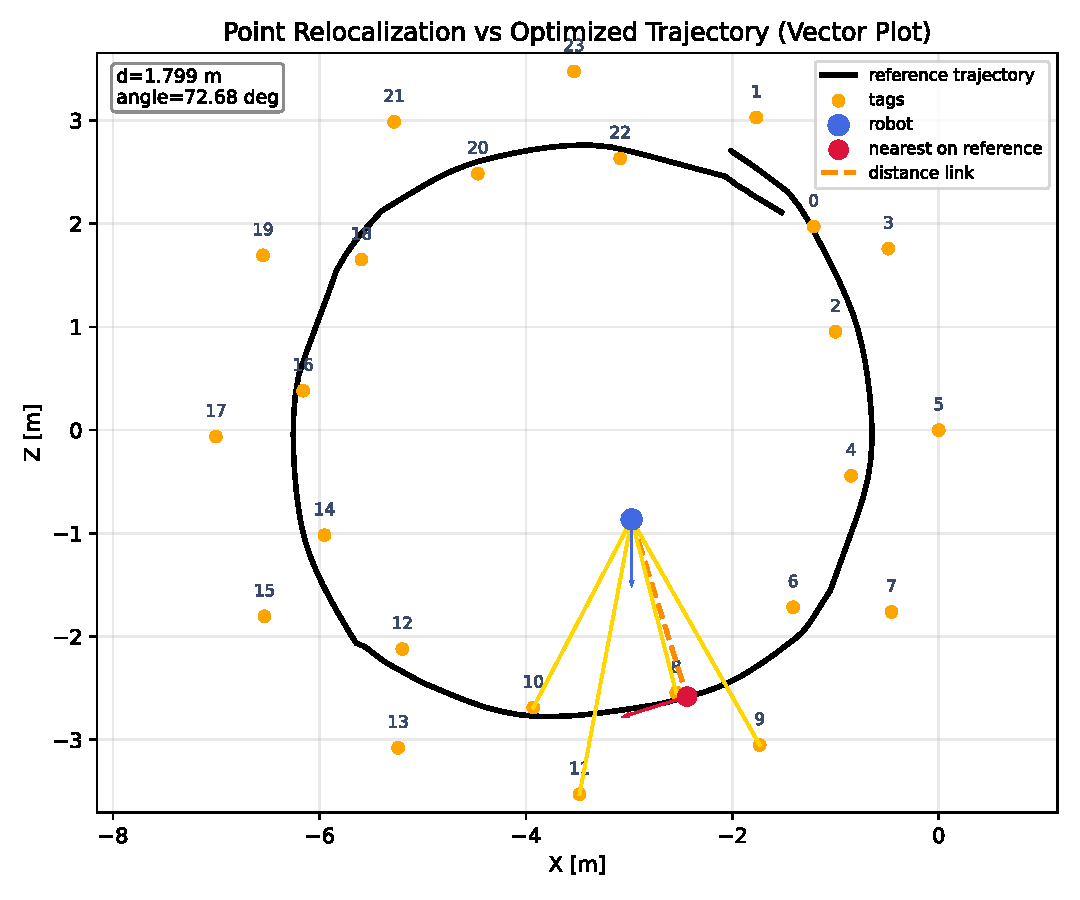
\includegraphics[width=\linewidth,height=0.65\textheight,keepaspectratio]{../Report/svg-inkscape/output_sim_between_tags_yz_08__relocalization_point_didactic_svg-raw.pdf}
    \end{column}
  \end{columns}
\end{frame}

\begin{frame}[label=appendix-mosaic-real-recording]{Real recording setup and corresponding reconstructed trajectory result.}
  \begin{columns}[c,onlytextwidth]
    \begin{column}{0.49\textwidth}
      \centering
      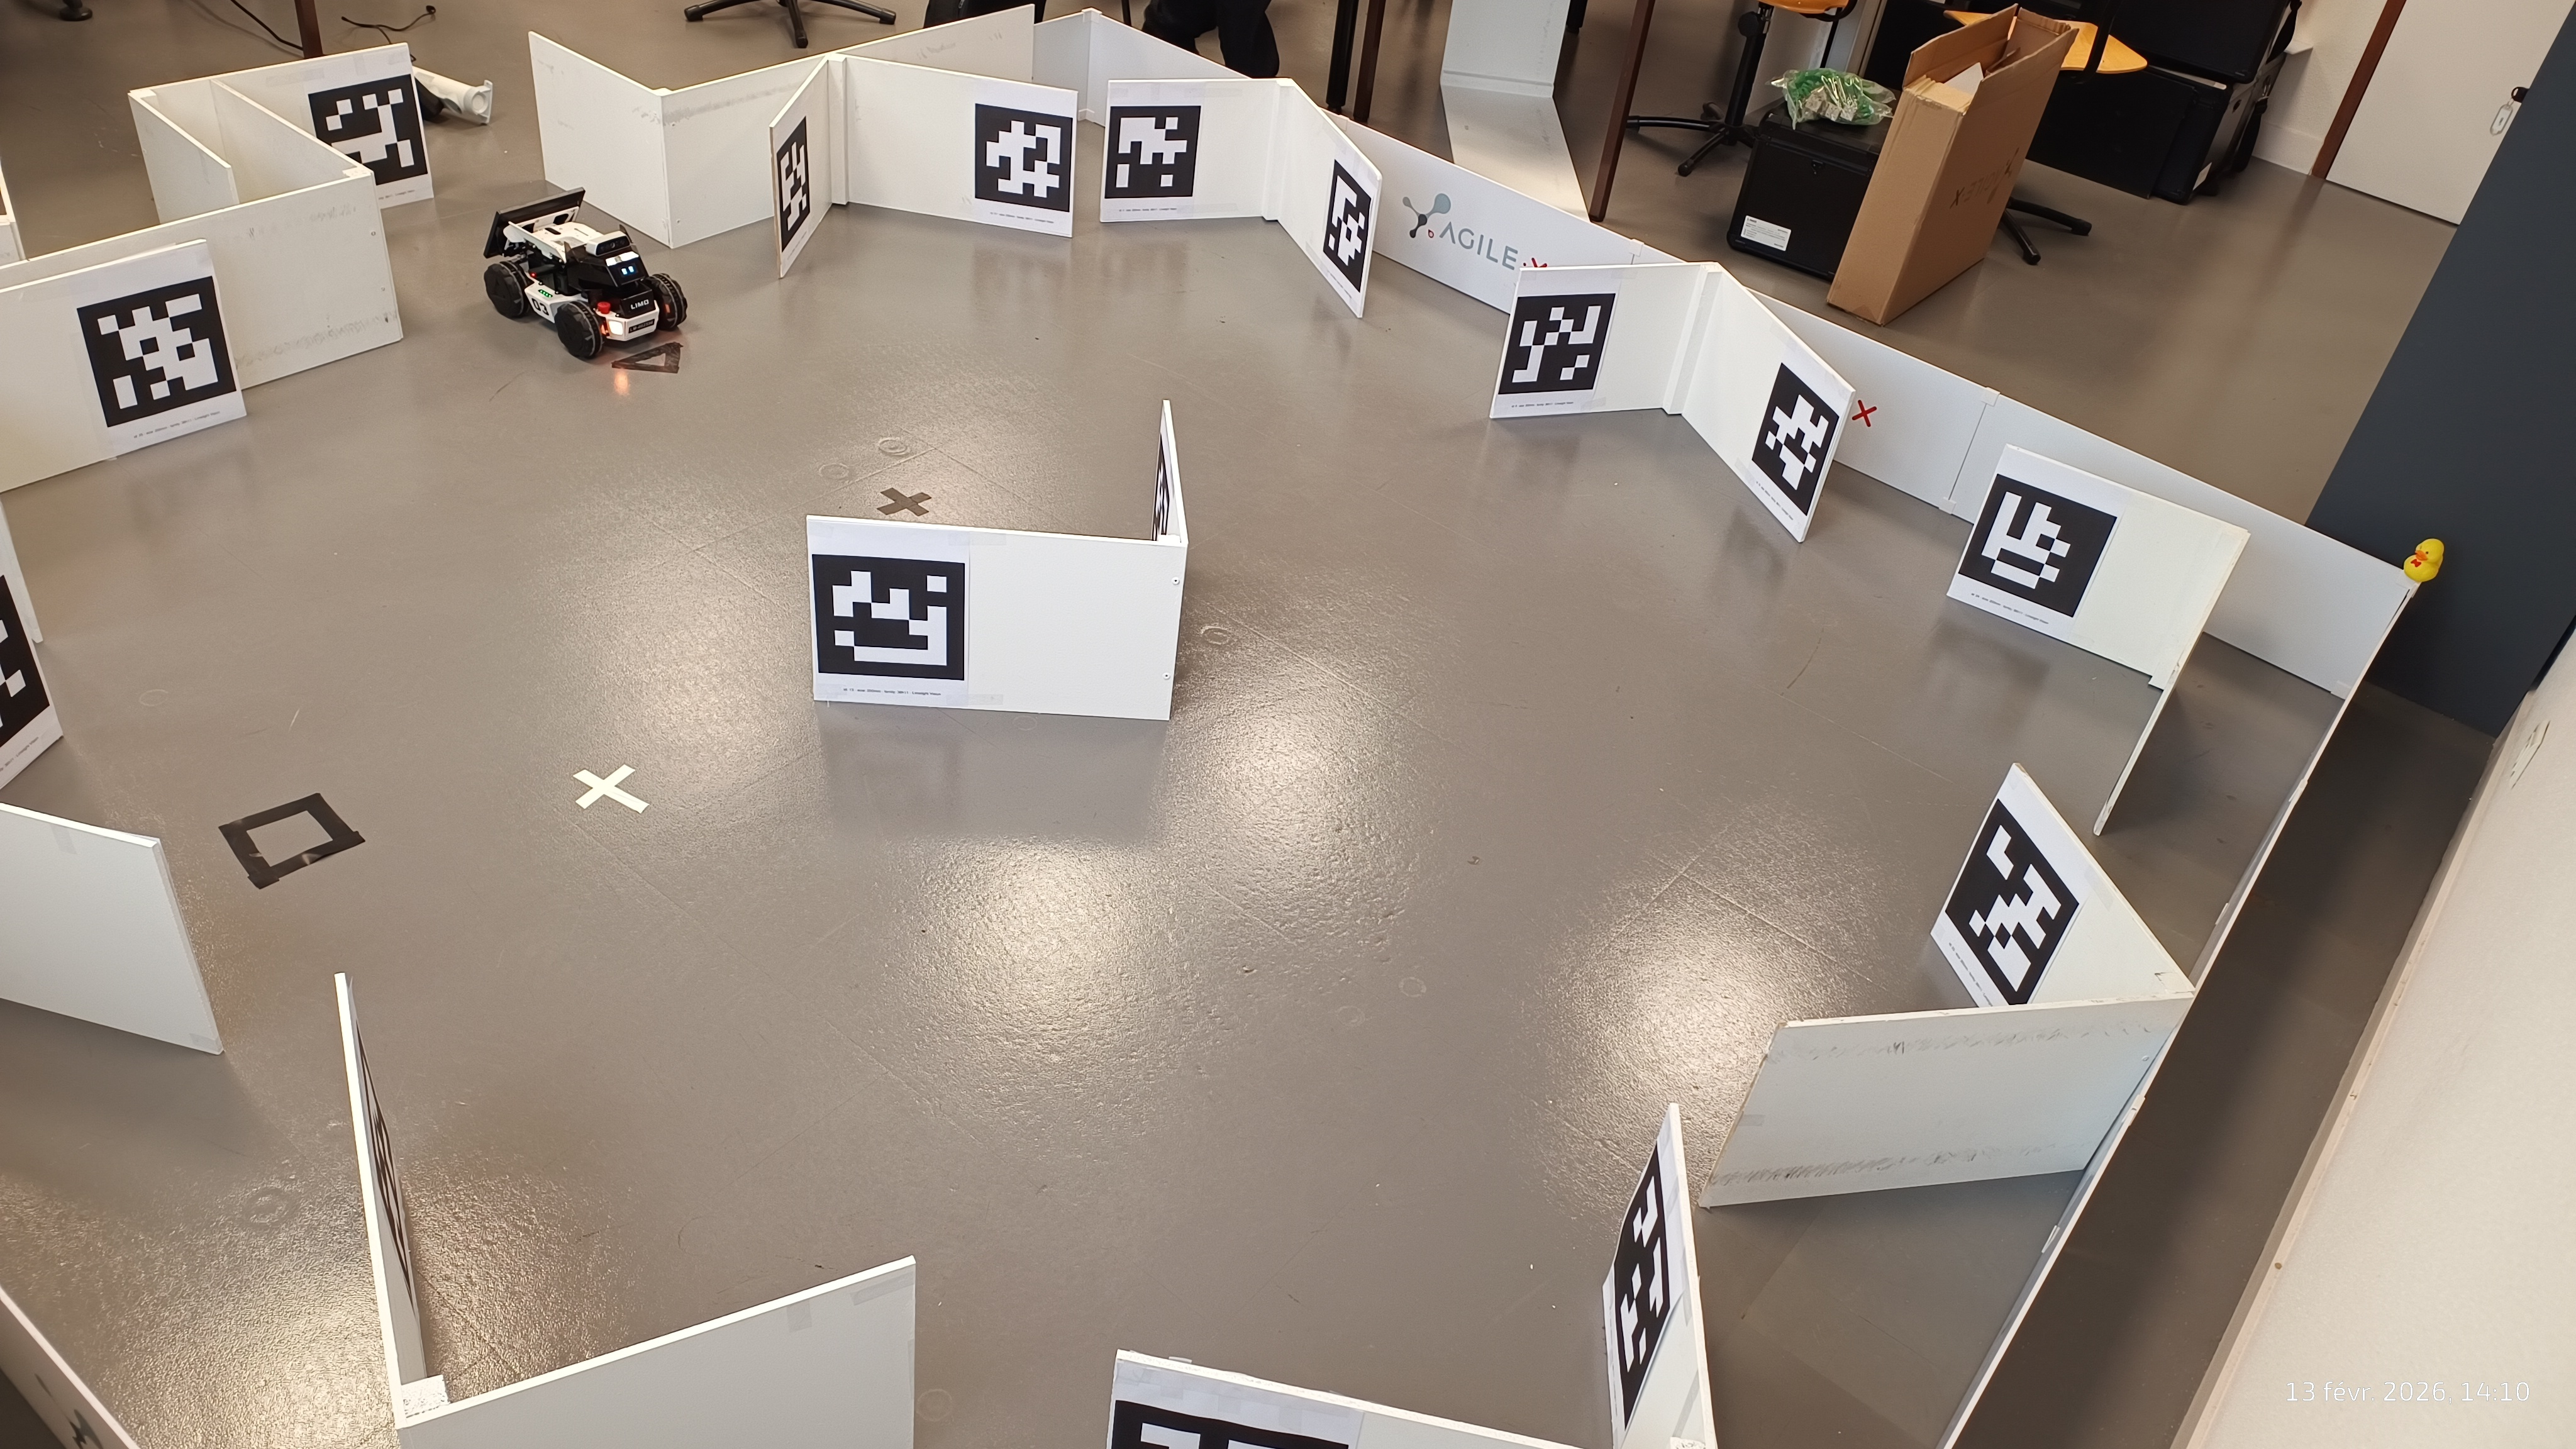
\includegraphics[width=\linewidth,height=0.65\textheight,keepaspectratio]{../Report/Images/recording_fase.jpg}
    \end{column}
    \begin{column}{0.49\textwidth}
      \centering
      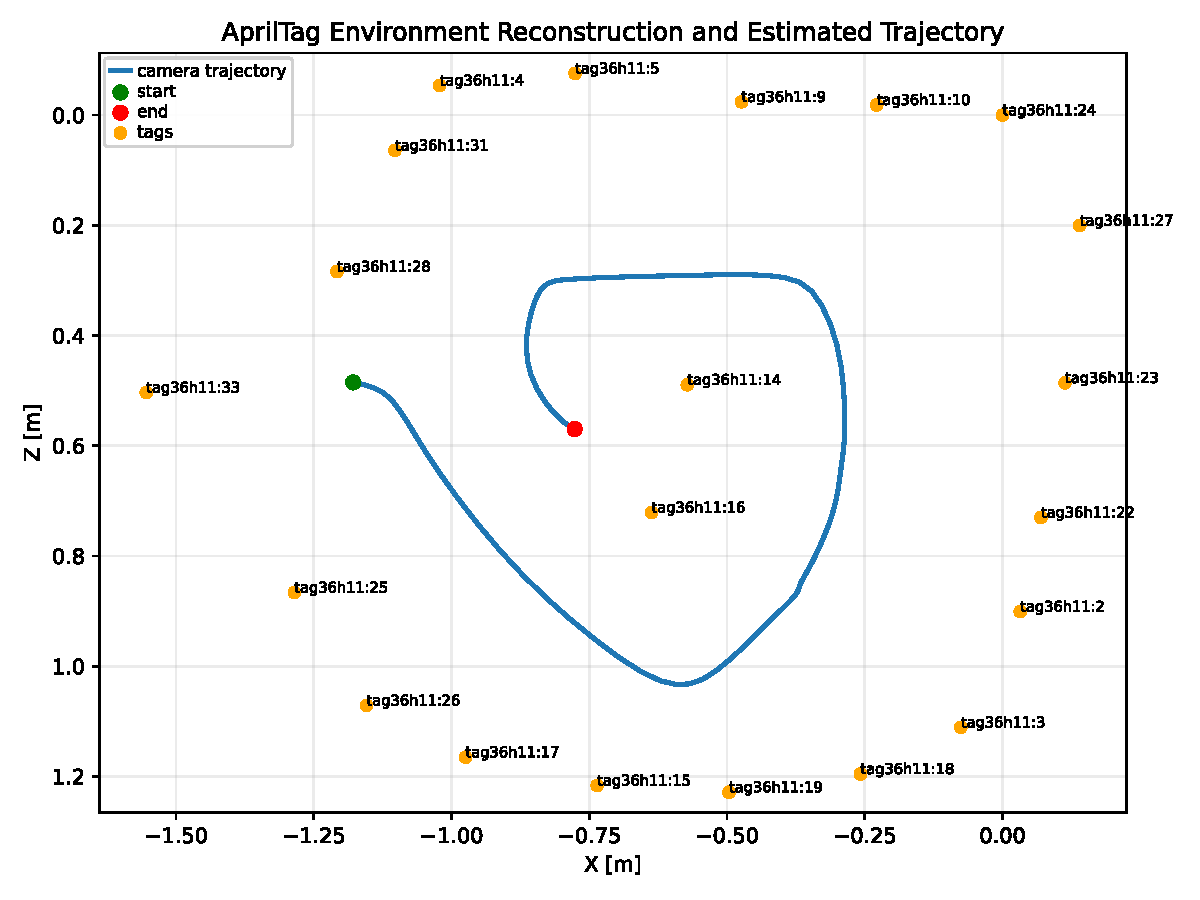
\includegraphics[width=\linewidth,height=0.65\textheight,keepaspectratio]{../Report/svg-inkscape/mapa_trajetoria_xz_svg-raw.pdf}
    \end{column}
  \end{columns}
\end{frame}

\begin{frame}[label=appendix-mosaic-real-relocal]{Real relocalization validation setup and corresponding distance comparison.}
  \begin{columns}[c,onlytextwidth]
    \begin{column}{0.49\textwidth}
      \centering
      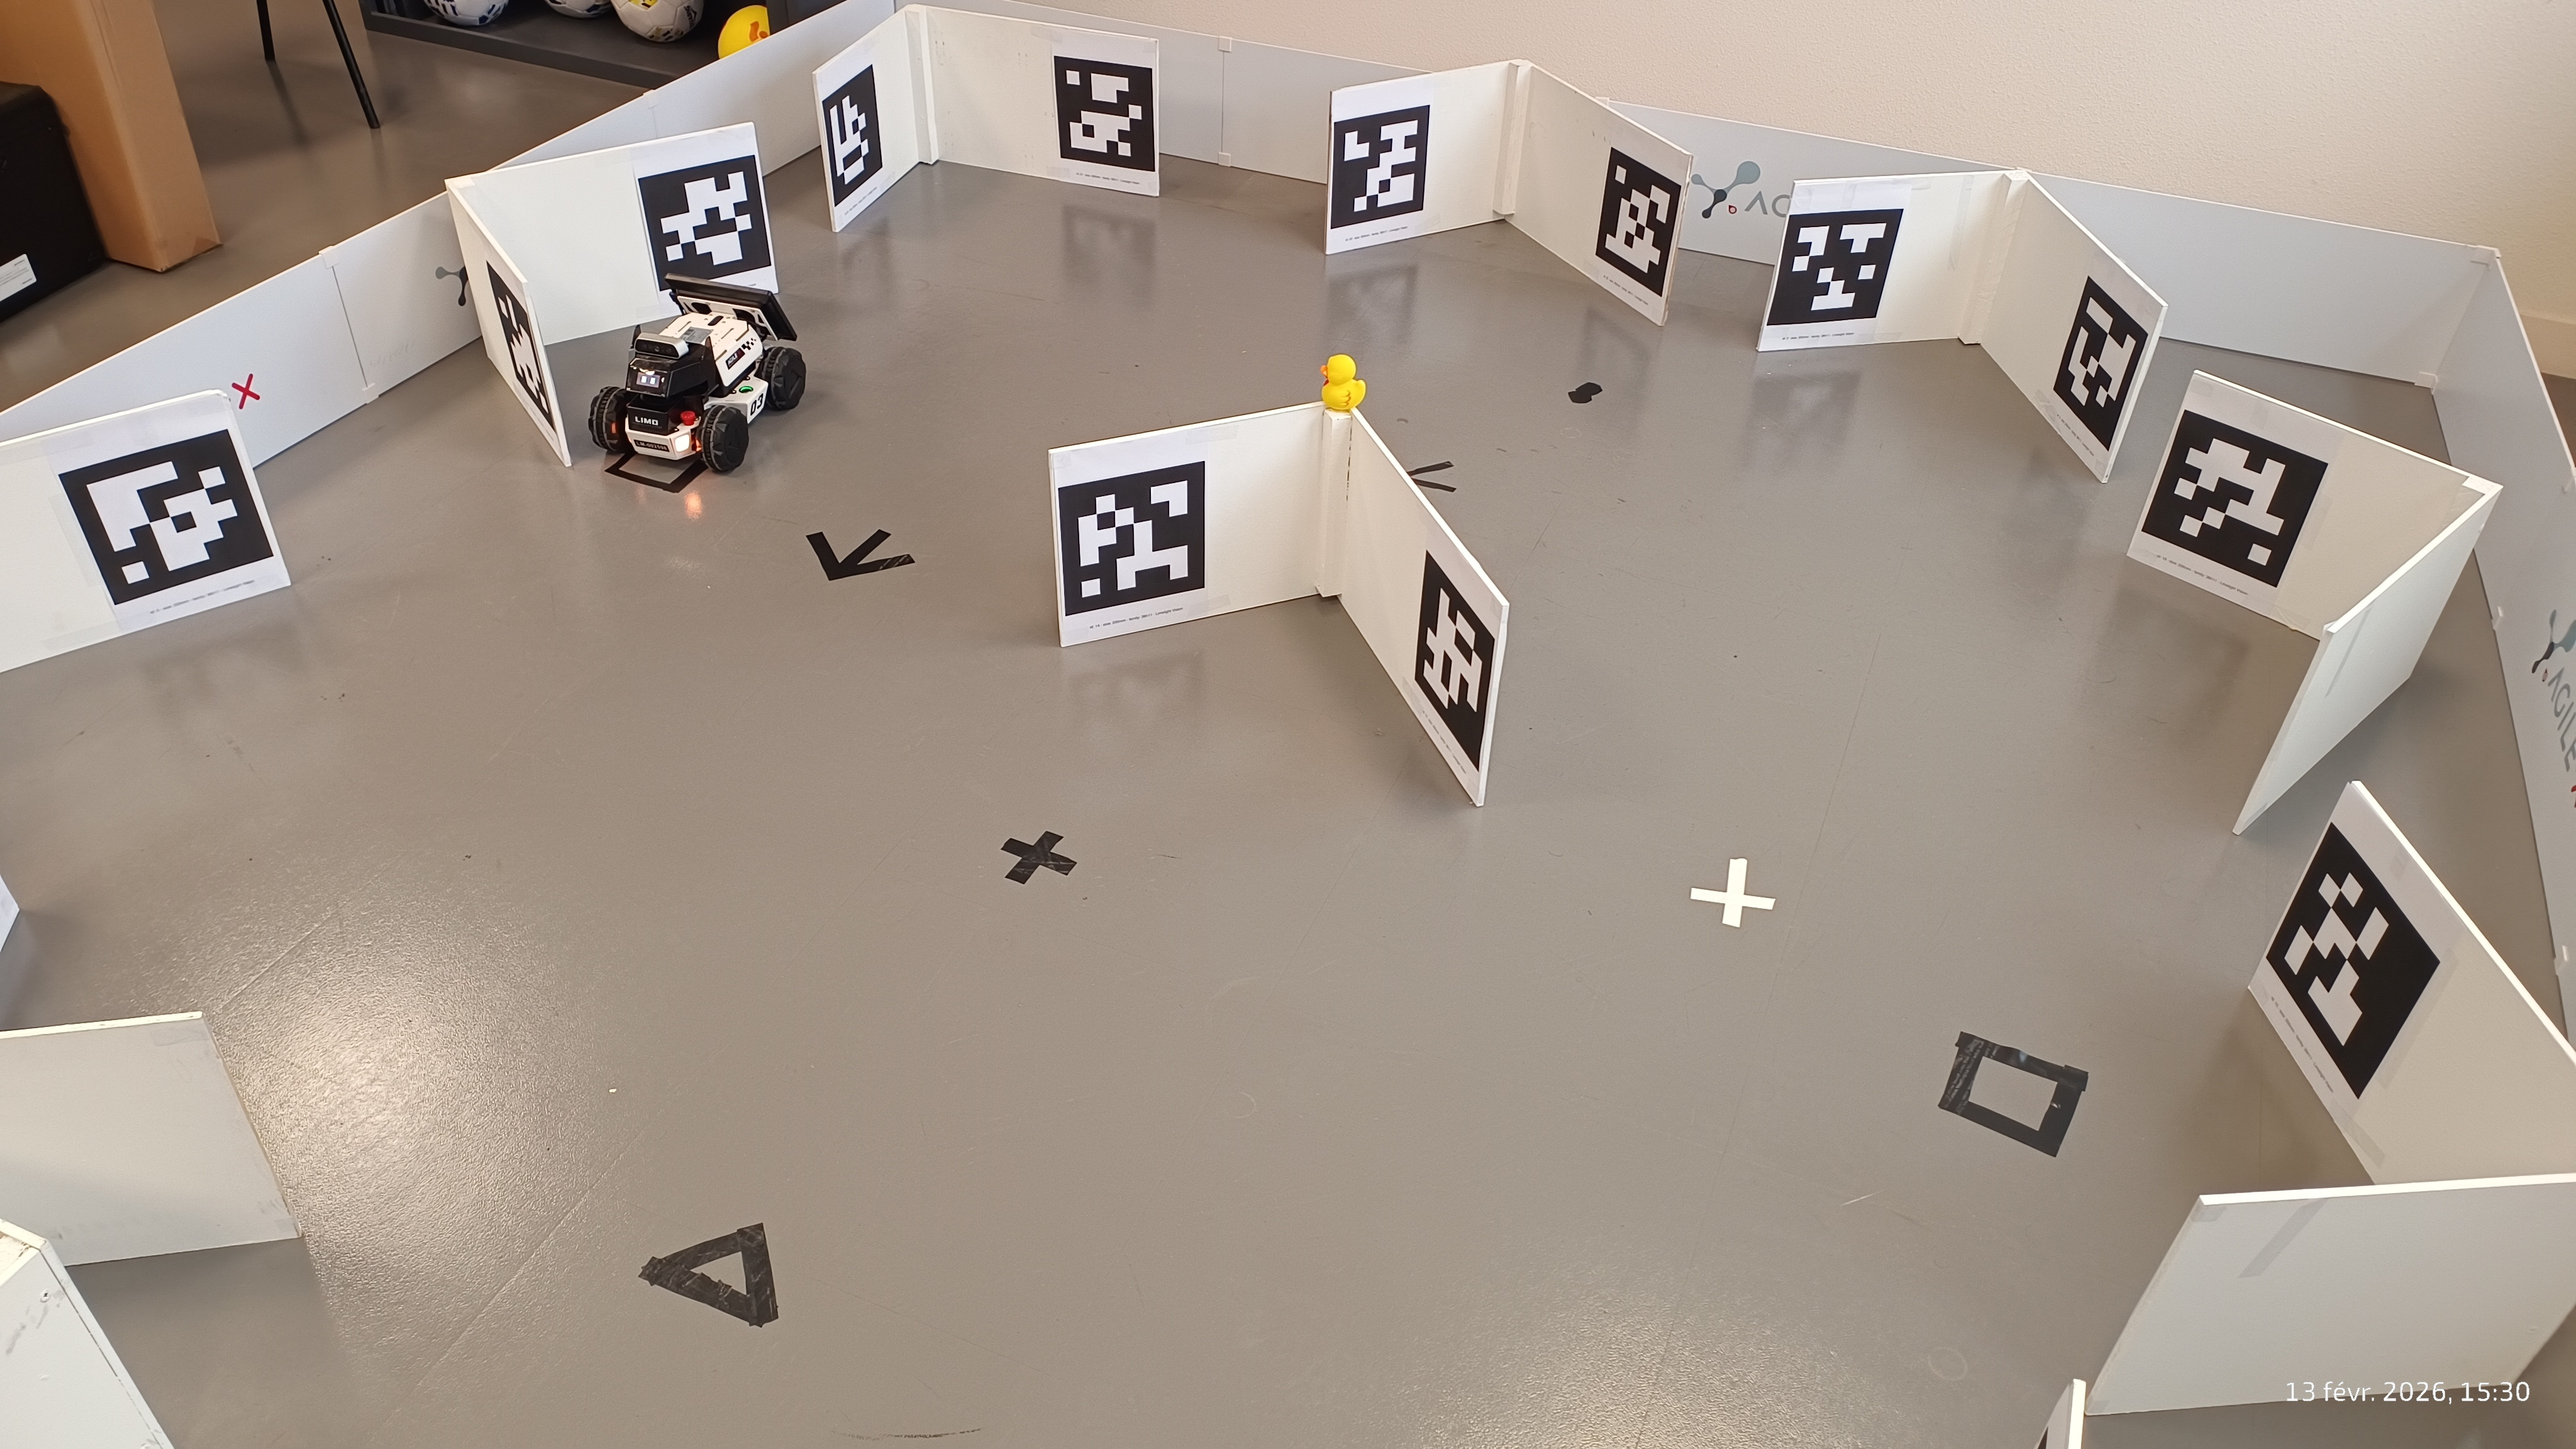
\includegraphics[width=\linewidth,height=0.65\textheight,keepaspectratio]{../Report/Images/relocalization_experiment.jpg}
    \end{column}
    \begin{column}{0.49\textwidth}
      \centering
      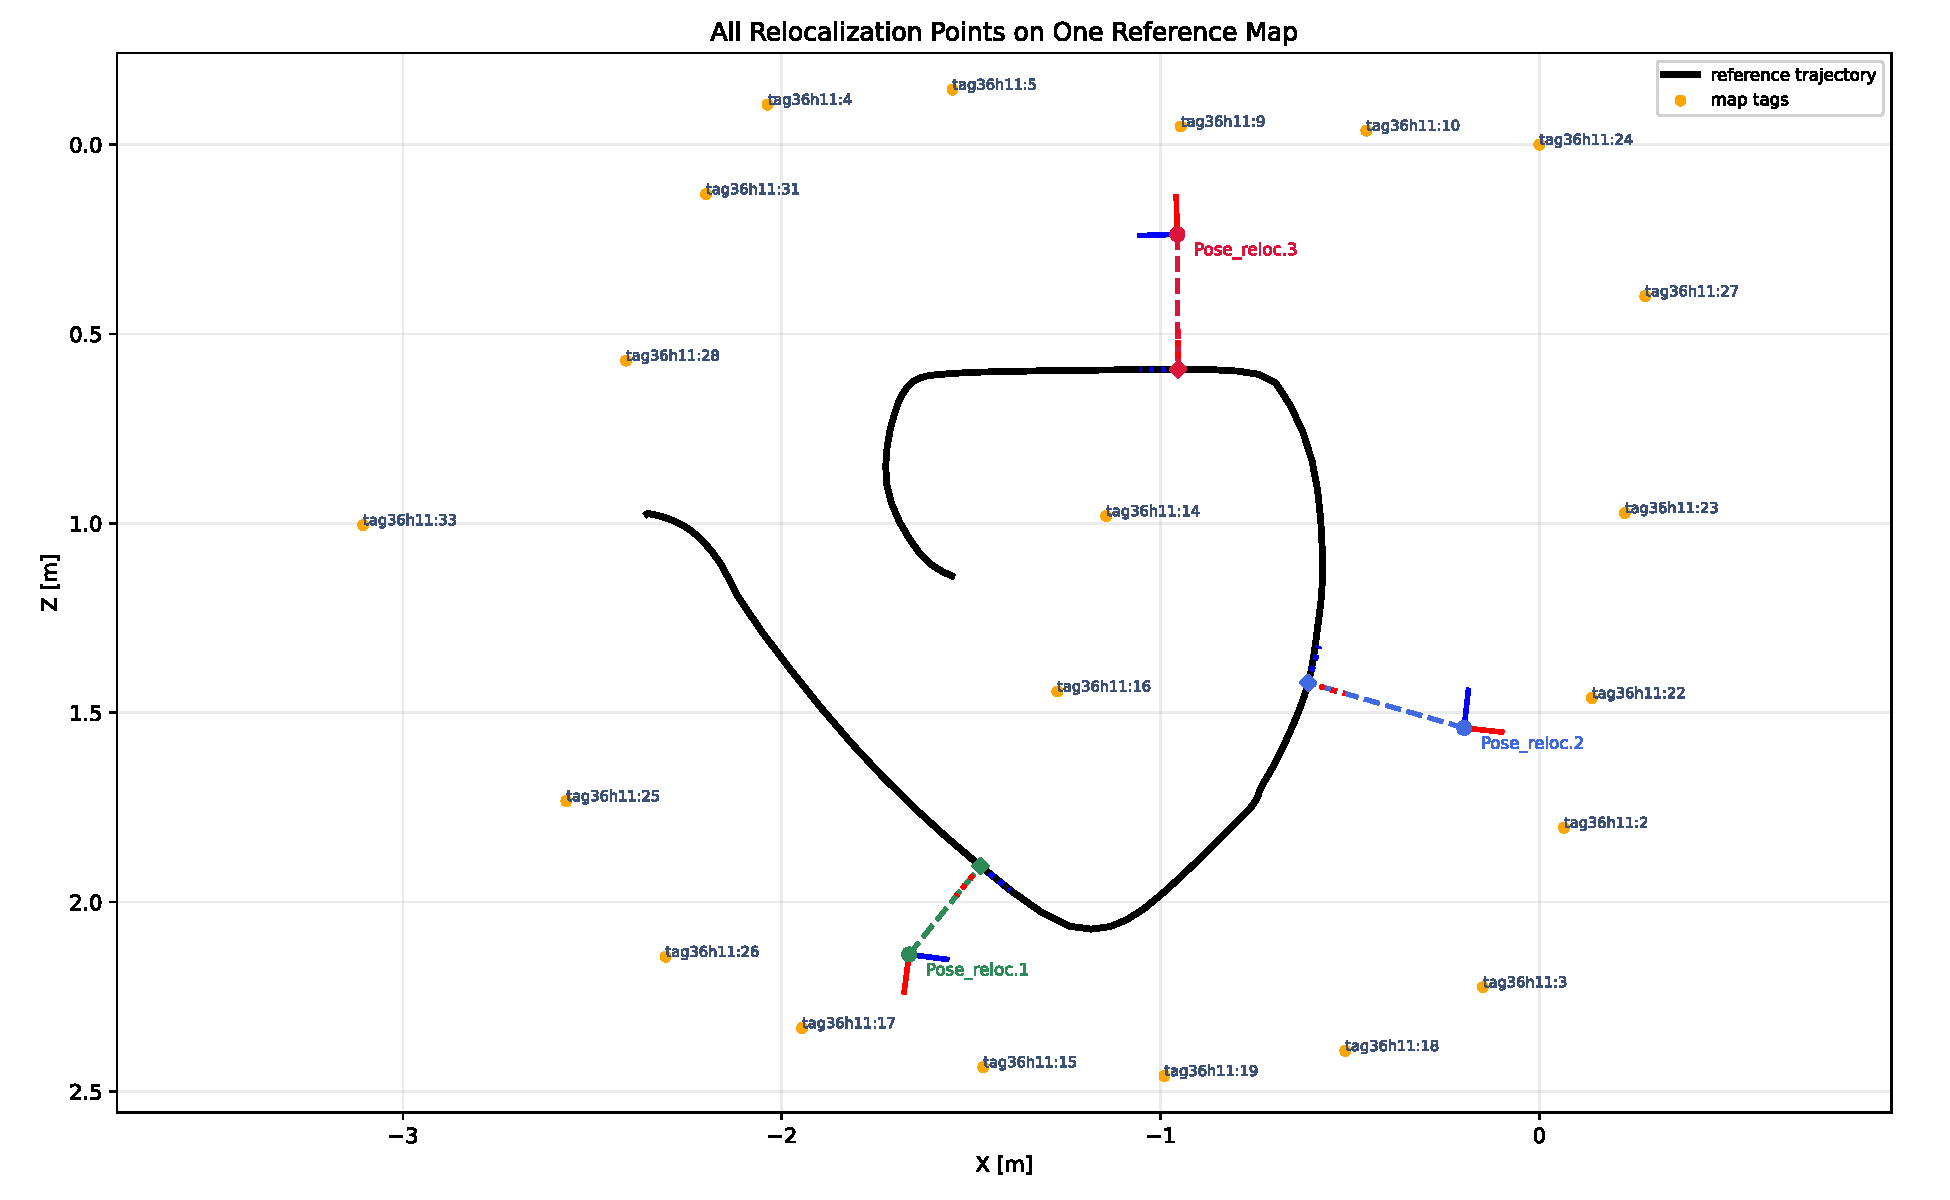
\includegraphics[width=\linewidth,height=0.65\textheight,keepaspectratio]{../Report/svg-inkscape/compare_three_letric_three_cases_points_svg-raw.pdf}
    \end{column}
  \end{columns}
\end{frame}

\begin{frame}[label=appendix-mosaic-second-recording]{Additional real recording result processed with the same offline pipeline.}
  \begin{columns}[c,onlytextwidth]
    \begin{column}{0.49\textwidth}
      \centering
      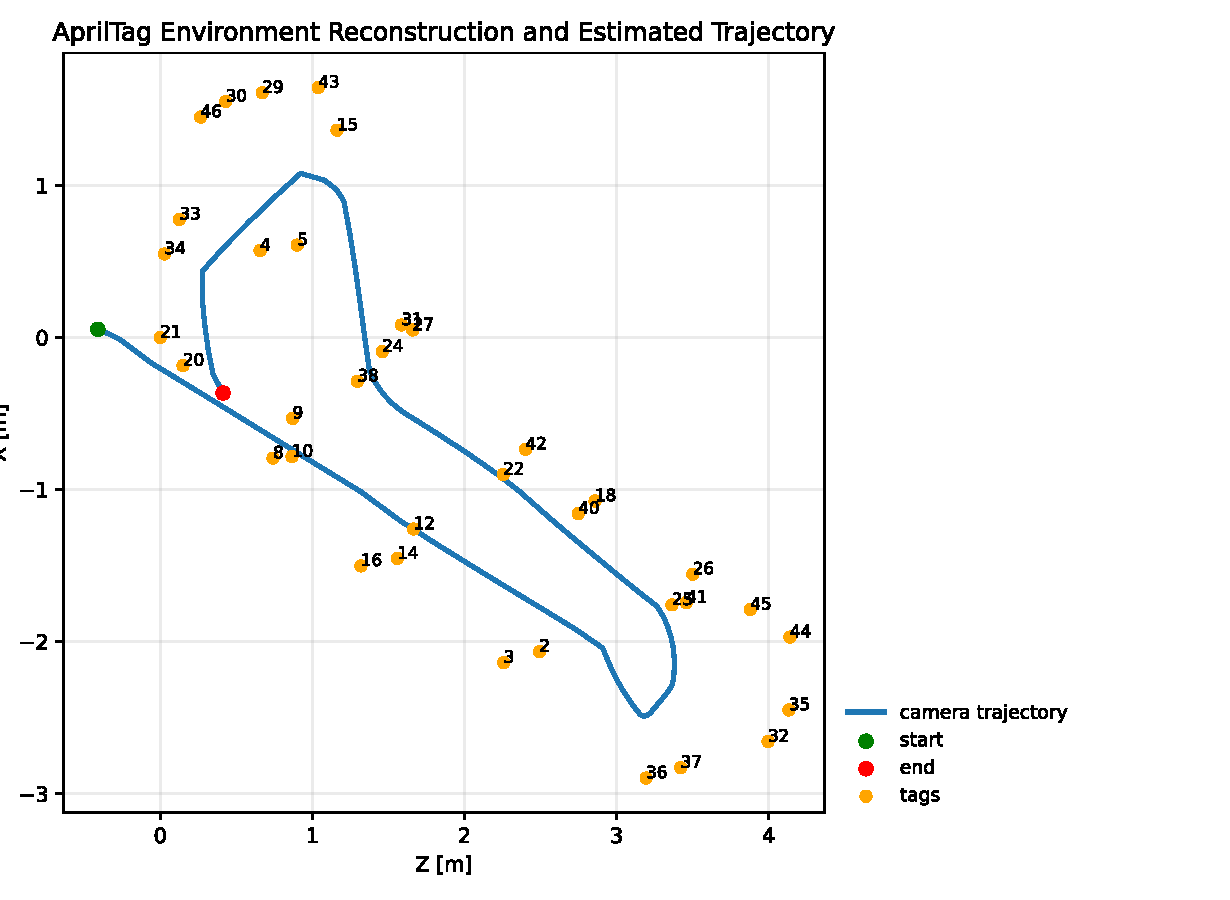
\includegraphics[width=\linewidth,height=0.65\textheight,keepaspectratio]{../Report/Images/output_020_recording_trajectory_basic.pdf}
    \end{column}
    \begin{column}{0.49\textwidth}
      \centering
      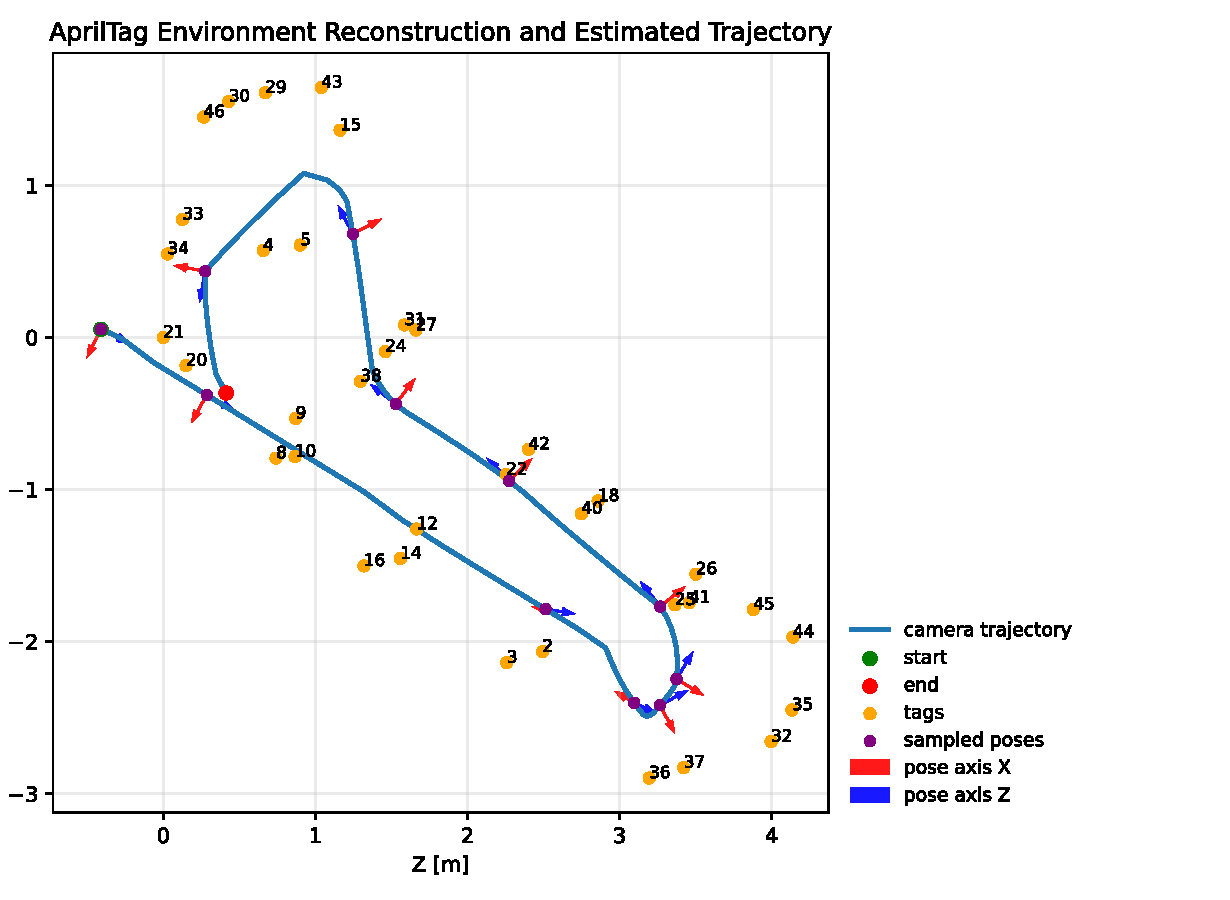
\includegraphics[width=\linewidth,height=0.65\textheight,keepaspectratio]{../Report/Images/output_020_recording_trajectory_with_axes.pdf}
    \end{column}
  \end{columns}
\end{frame}

\begin{frame}[label=appendix-discussion-recording-limitations]{Discussion - Recording Limitations}
\transfade[duration=0.25]
\vspace{-0.08cm}
\begin{outlinecard}[Error Summary Across Validations]
  \scriptsize
  \centering
  \begin{tabular}{lcc}
    \toprule
    \textbf{Validation Case} & \textbf{Traj. Mean Error [m]} & \textbf{Tag/Map Mean Error [m]} \\
    \midrule
    Synthetic (noise-free) & 0.0000 & 0.0000 \\
    Synthetic (+10 cm noise) & 0.0584 & 0.0364 \\
    Simulation & 0.0510 & 0.0873 \\
    Real recording & -- & 0.0390 \\
    \bottomrule
  \end{tabular}
\end{outlinecard}

\vspace{-0.05cm}
\begin{outlinecard}[Reading Notes]
  \small
  \begin{itemize}
    \item Real: map consistency (no full GT).
    \item Sensitive to visibility and calibration.
  \end{itemize}
\end{outlinecard}
\end{frame}

\tikzset{
  appbase/.style={draw=NavyBlue!80, thick, align=center, inner sep=4pt, font=\scriptsize},
  appio/.style={appbase, trapezium, trapezium left angle=70, trapezium right angle=110, fill=AccentBlue!12},
  appproc/.style={appbase, rectangle, rounded corners=1mm, fill=gray!8},
  apppose/.style={appbase, rectangle, rounded corners=1mm, fill=NavyBlue!10},
  appstore/.style={appbase, trapezium, trapezium left angle=70, trapezium right angle=110, fill=gray!8},
  apparrow/.style={-Stealth, thick, draw=NavyBlue!80},
}

\begin{frame}[label=appendix-flowchart-recording]{Architecture of the offline recording pipeline.}
\centering
\resizebox{0.95\linewidth}{!}{
\begin{tikzpicture}[node distance=10mm and 14mm]
  \node[appio] (bag) {Logging dataset\\\textit{rosbag2}};
  \node[appproc, below left=12mm and 6mm of bag] (det) {Detections\\AprilTag};
  \node[appproc, below right=12mm and 6mm of bag] (cam) {Camera intrinsics\\Camera\_Info};
  \node[apppose, right=18mm of bag] (pnp) {\textbf{(1)} Pose estimation (PnP)};
  \node[appproc, right=12mm of pnp] (pair) {\textbf{(2)} Pairwise constraints};
  \node[apppose, right=12mm of pair] (map) {\textbf{(3)} Tag map optimization};
  \node[apppose, below=10mm of map] (traj) {\textbf{(4)} Reference trajectory\\(+ smoothing)};
  \node[appstore, right=12mm of map] (out) {Exports\\tag\_map.yaml/csv\\trajetoria\_camera.csv};
  \draw[apparrow] (det) -- (bag);
  \draw[apparrow] (cam) -- (bag);
  \draw[apparrow] (bag) -- (pnp);
  \draw[apparrow] (pnp) -- (pair);
  \draw[apparrow] (pair) -- (map);
  \draw[apparrow] (map) -- (out);
  \draw[apparrow] (map) -- (traj);
  \draw[apparrow] (traj.east) -| (out.south);
\end{tikzpicture}
}
\end{frame}

\begin{frame}[label=appendix-flowchart-relocal]{Architecture of the relocalization pipeline with separated offline analysis and online execution.}
\centering
\resizebox{0.95\linewidth}{!}{
\begin{tikzpicture}[node distance=10mm and 12mm]
  \node[appstore] (reftraj) {Reference trajectory\\trajetoria\_camera.csv};
  \node[appstore, right=12mm of reftraj] (refmap) {Tag map\\tag\_map.yaml/csv};
  \node[appio, below=14mm of reftraj] (qoff) {Query poses\\(offline dataset)};
  \node[appproc, right=10mm of qoff] (align) {\textbf{(1)} Optional planar\\alignment};
  \node[apppose, right=10mm of align] (nearoff) {\textbf{(2)} Nearest point\\search};
  \node[apppose, right=10mm of nearoff] (erroff) {\textbf{(3)} Compute\\$D$ and $\phi$};
  \node[appstore, right=10mm of erroff] (report) {Exports\\metrics/plots};
  \node[appio, below=12mm of qoff] (live) {Estimated robot pose\\(online)};
  \node[appproc, right=10mm of live] (load) {\textbf{(4*)} Load\\reference};
  \node[apppose, right=10mm of load] (nearon) {\textbf{(5)} Nearest\\point+tangent};
  \node[apppose, right=10mm of nearon] (erron) {\textbf{(6)} Output\\$D$ and $\phi$};
  \node[appstore, right=10mm of erron] (topics) {ROS topics\\distance, heading};
  \draw[apparrow] (reftraj.south) -- (qoff.north);
  \draw[apparrow] (refmap.south) -- (align.north);
  \draw[apparrow] (qoff) -- (align) -- (nearoff) -- (erroff) -- (report);
  \draw[apparrow] (live) -- (load) -- (nearon) -- (erron) -- (topics);
\end{tikzpicture}
}
\end{frame}

\begin{frame}[label=appendix-table-20]{Table 2.0: Functional Requirements}
\scriptsize
\centering
\begin{tabular}{|c|p{0.79\linewidth}|}
\hline
\textbf{ID} & \textbf{Requirement} \\ \hline
FR1 & The system shall provide workflows for recording robot motion and perception data into rosbag2 datasets for offline processing. \\ \hline
FR2 & The system shall process recorded rosbag2 datasets offline to generate a reference trajectory and a spatial map of detected AprilTags. \\ \hline
FR3 & The offline processing stage shall export structured output files, including trajectory CSV and tag map YAML/CSV formats. \\ \hline
FR4 & The system shall provide an online relocalization node capable of loading a reference trajectory, subscribing to a live pose topic, computing nearest-point distance and heading deviation, and publishing these quantities for controller integration. \\ \hline
FR5 & The system shall publish visualization-compatible ROS topics enabling RViz display of reference trajectory, current pose, nearest reference pose, and relocalization error indicators. \\ \hline
FR6 & The system shall provide launch files and profile scripts supporting both real and simulation workflows. \\ \hline
FR7 & The system shall include documented execution procedures ensuring reproducibility from recorded datasets. \\ \hline
\end{tabular}
\end{frame}

\begin{frame}[label=appendix-table-21]{Table 2.1: Non-Functional Requirements}
\scriptsize
\centering
\begin{tabular}{|c|p{0.79\linewidth}|}
\hline
\textbf{ID} & \textbf{Requirement} \\ \hline
NFR1 & Offline reconstruction shall be executable independently of live robot operation. \\ \hline
NFR2 & Online relocalization shall operate within computational limits compatible with real-time ROS~2 execution. \\ \hline
NFR3 & The architecture shall maintain separation between perception, offline reconstruction, and online relocalization components. \\ \hline
NFR4 & The system shall ensure consistency of coordinate frames within the ROS~2 TF structure. \\ \hline
NFR5 & Dataset files shall remain external to version control to maintain repository portability. \\ \hline
\end{tabular}
\end{frame}

\begin{frame}[label=appendix-table-22]{Table 2.2: Project Deliverables and Constraints}
\scriptsize
\centering
\begin{tabular}{|c|p{0.79\linewidth}|}
\hline
\textbf{ID} & \textbf{Requirement} \\ \hline
PR1 & The project shall be delivered as a version-controlled ROS~2 workspace repository containing source code, launch files, scripts, and documentation. \\ \hline
PR2 & The repository shall include structured workflows for both real and simulation execution. \\ \hline
C1 & The system shall be implemented in ROS~2 Humble. \\ \hline
C2 & The perception pipeline shall use AprilTag v3 with the tag36h11 family. \\ \hline
C3 & Experimental validation shall be conducted on the AgileX LIMO platform. \\ \hline
C4 & The system shall not include full autonomous navigation, SLAM of unknown environments, obstacle avoidance, or mission-level planning. \\ \hline
\end{tabular}
\end{frame}

\begin{frame}[label=appendix-table-23]{Table 2.3: Technical Limitations}
\scriptsize
\centering
\begin{tabular}{|c|p{0.79\linewidth}|}
\hline
\textbf{ID} & \textbf{Limitation} \\ \hline
TL1 & Accurate and stable pose estimation assumes that at least two AprilTags are simultaneously visible in the camera field of view. While pose can be computed from a single detection, multi-tag observations improve numerical stability and reduce sensitivity to noise and calibration errors. \\ \hline
TL2 & Localization precision depends on camera calibration quality, tag size, distance to the tags, and image resolution. The system does not guarantee fixed absolute accuracy under arbitrary environmental conditions. \\ \hline
\end{tabular}
\end{frame}

\begin{frame}[label=appendix-table-41]{Table 4.1: Residual errors in the ideal scenario (no noise).}
\small
\centering
\begin{tabular}{|l|c|c|c|}
\hline
\textbf{Metric} & \textbf{Mean Error} & \textbf{Minimum} & \textbf{Maximum} \\ \hline
Camera Trajectory & $0.0000\text{ m} / 0.00^\circ$ & $0.0000\text{ m} / 0.00^\circ$ & $0.0000\text{ m} / 0.00^\circ$ \\ \hline
Tag Poses & $0.0000\text{ m} / 0.00^\circ$ & $0.0000\text{ m} / 0.00^\circ$ & $0.0000\text{ m} / 0.00^\circ$ \\ \hline
\end{tabular}
\end{frame}

\begin{frame}[label=appendix-table-42]{Table 4.2: Error statistics under 10 cm Gaussian noise.}
\small
\centering
\begin{tabular}{|l|c|c|c|}
\hline
\textbf{Metric} & \textbf{Mean Error} & \textbf{Minimum} & \textbf{Maximum} \\ \hline
Camera Trajectory & $0.0584\text{ m} / 0.97^\circ$ & $0.0126\text{ m} / 0.11^\circ$ & $0.1485\text{ m} / 2.67^\circ$ \\ \hline
Tag Poses & $0.0364\text{ m} / 0.73^\circ$ & $0.0156\text{ m} / 0.73^\circ$ & $0.0583\text{ m} / 0.73^\circ$ \\ \hline
\end{tabular}
\end{frame}

\begin{frame}[label=appendix-table-43]{Table 4.3: Summary table with estimated versus measured distance to the recorded trajectory and the estimated heading offset $\phi$.}
\small
\centering
\begin{tabular}{|c|c|c|c|c|}
\hline
\textbf{Relocalization Case} & \textbf{Estimated D [m]} & \textbf{Measured D [m]} & \textbf{Error [m]} & \textbf{$\phi$ [deg]} \\ \hline
1 & 0.2998 & 0.3100 & 0.0102 & -31.38 \\ \hline
2 & 0.4284 & 0.4200 & 0.0084 & -10.34 \\ \hline
3 & 0.3567 & 0.3600 & 0.0033 & -1.63 \\ \hline
\end{tabular}
\end{frame}

\begin{frame}[label=appendix-table-a1]{Table A.1: Comparison between estimated and measured distances from tag 16.}
\tiny
\centering
\scalebox{0.68}{%
\begin{tabular}{|c|c|c|c|c|}
\hline
\textbf{Source tag} & \textbf{Target tag} & \textbf{Estimated [m]} & \textbf{Measured [m]} & \textbf{Absolute error [m]} \\ \hline
16 & 2 & 1.385 & 1.380 & 0.005 \\ \hline
16 & 3 & 1.368 & 1.360 & 0.008 \\ \hline
16 & 4 & 1.728 & 1.820 & 0.092 \\ \hline
16 & 5 & 1.613 & 1.690 & 0.077 \\ \hline
16 & 9 & 1.527 & 1.450 & 0.077 \\ \hline
16 & 10 & 1.691 & 1.680 & 0.011 \\ \hline
16 & 14 & 0.481 & 0.480 & 0.001 \\ \hline
16 & 15 & 1.011 & 1.110 & 0.099 \\ \hline
16 & 17 & 1.115 & 1.090 & 0.025 \\ \hline
16 & 18 & 1.216 & 1.220 & 0.004 \\ \hline
16 & 19 & 1.054 & 1.040 & 0.014 \\ \hline
16 & 22 & 1.412 & 1.410 & 0.002 \\ \hline
16 & 23 & 1.571 & 1.560 & 0.011 \\ \hline
16 & 24 & 1.925 & 1.900 & 0.025 \\ \hline
16 & 25 & 1.328 & 1.300 & 0.028 \\ \hline
16 & 26 & 1.249 & 1.220 & 0.029 \\ \hline
16 & 27 & 1.871 & 1.800 & 0.071 \\ \hline
16 & 28 & 1.436 & 1.470 & 0.034 \\ \hline
16 & 31 & 1.608 & 1.660 & 0.052 \\ \hline
16 & 33 & 1.886 & 1.870 & 0.016 \\ \hline
\textbf{Mean} & - & - & - & \textbf{0.039} \\ \hline
\textbf{Max} & - & - & - & \textbf{0.099} \\ \hline
\textbf{Min} & - & - & - & \textbf{0.001} \\ \hline
\end{tabular}
}
\end{frame}

\edef\MediaRelocDemoOneFile{\detokenize{assets/reloc_demo1.webm}}
\edef\MediaRelocDemoTwoFile{\detokenize{assets/reloc_demo2.webm}}
\edef\MediaRelocRealScenarioOneFile{\detokenize{assets/reloc_real_scneario_1.webm}}
\edef\MediaRelocScenarioTwoFile{\detokenize{assets/Reloc_scnerio2.webm}}
\edef\MediaTrajectoryOneFile{\detokenize{assets/trajetory_1_4x_cropped.mp4}}
\edef\MediaRelocDemoOneThumb{\detokenize{assets/media_reloc_demo1_thumb.jpg}}
\edef\MediaRelocDemoTwoThumb{\detokenize{assets/media_reloc_demo2_thumb.jpg}}
\edef\MediaRelocRealScenarioOneThumb{\detokenize{assets/media_reloc_real1_thumb.jpg}}
\edef\MediaRelocScenarioTwoThumb{\detokenize{assets/media_reloc_scn2_thumb.jpg}}
\edef\MediaTrajectoryOneThumb{\detokenize{assets/media_traj1_thumb.jpg}}
\edef\MediaValidationExpTwoFile{\detokenize{assets/trajetory_2_5x_cropped.mp4}}
\edef\MediaValidationExpTwoThumb{\detokenize{assets/trajetory_2_thumb.jpg}}

\begin{frame}[label=appendix-media-validation-exp2]{Appendix Media - Validation Experiment 2 (Large)}
\centering
\vspace{0.05cm}
\IfFileExists{\MediaValidationExpTwoFile}{
  \movie[
    width=0.60\linewidth,
    height=0.45\linewidth,
    poster
  ]{%
    \fcolorbox{NavyBlue}{white}{%
      \includegraphics[
        width=\dimexpr0.60\linewidth-2\fboxrule\relax,
        height=\dimexpr0.45\linewidth-2\fboxrule\relax,
        keepaspectratio
      ]{\MediaValidationExpTwoThumb}%
    }%
  }{\MediaValidationExpTwoFile}
}{
  \begin{alertbox}[Video Missing]
    Add the file \texttt{\MediaValidationExpTwoFile}.
  \end{alertbox}
}
\end{frame}

\begin{frame}[label=appendix-media-reloc-demo1]{Appendix Media - reloc\_demo1.webm}
\centering
\IfFileExists{\MediaRelocDemoOneFile}{
  \movie[
    width=0.92\linewidth,
    height=0.24\linewidth,
    poster
  ]{%
    \fcolorbox{NavyBlue}{white}{\includegraphics[width=\linewidth,height=0.24\linewidth,keepaspectratio]{\MediaRelocDemoOneThumb}}%
  }{\MediaRelocDemoOneFile}
}{
  \begin{alertbox}[Video Missing]
    Add the file \texttt{\MediaRelocDemoOneFile}.
  \end{alertbox}
}
\end{frame}

\begin{frame}[label=appendix-media-reloc-demo2]{Appendix Media - reloc\_demo2.webm}
\centering
\IfFileExists{\MediaRelocDemoTwoFile}{
  \movie[
    width=0.92\linewidth,
    height=0.24\linewidth,
    poster
  ]{%
    \fcolorbox{NavyBlue}{white}{\includegraphics[width=\linewidth,height=0.24\linewidth,keepaspectratio]{\MediaRelocDemoTwoThumb}}%
  }{\MediaRelocDemoTwoFile}
}{
  \begin{alertbox}[Video Missing]
    Add the file \texttt{\MediaRelocDemoTwoFile}.
  \end{alertbox}
}
\end{frame}

\begin{frame}[label=appendix-media-reloc-real1]{Appendix Media - reloc\_real\_scneario\_1.webm}
\centering
\IfFileExists{\MediaRelocRealScenarioOneFile}{
  \movie[
    width=0.92\linewidth,
    height=0.43\linewidth,
    poster
  ]{%
    \fcolorbox{NavyBlue}{white}{\includegraphics[width=\linewidth,height=0.43\linewidth,keepaspectratio]{\MediaRelocRealScenarioOneThumb}}%
  }{\MediaRelocRealScenarioOneFile}
}{
  \begin{alertbox}[Video Missing]
    Add the file \texttt{\MediaRelocRealScenarioOneFile}.
  \end{alertbox}
}
\end{frame}

\begin{frame}[label=appendix-media-reloc-scn2]{Appendix Media - Reloc\_scnerio2.webm}
\centering
\IfFileExists{\MediaRelocScenarioTwoFile}{
  \movie[
    width=0.92\linewidth,
    height=0.43\linewidth,
    poster
  ]{%
    \fcolorbox{NavyBlue}{white}{\includegraphics[width=\linewidth,height=0.43\linewidth,keepaspectratio]{\MediaRelocScenarioTwoThumb}}%
  }{\MediaRelocScenarioTwoFile}
}{
  \begin{alertbox}[Video Missing]
    Add the file \texttt{\MediaRelocScenarioTwoFile}.
  \end{alertbox}
}
\end{frame}

\begin{frame}[label=appendix-media-traj1]{Appendix Media - trajetory\_1\_4x\_cropped.mp4}
\centering
\IfFileExists{\MediaTrajectoryOneFile}{
  \movie[
    width=0.92\linewidth,
    height=0.44\linewidth,
    poster
  ]{%
    \fcolorbox{NavyBlue}{white}{\includegraphics[width=\linewidth,height=0.44\linewidth,keepaspectratio]{\MediaTrajectoryOneThumb}}%
  }{\MediaTrajectoryOneFile}
}{
  \begin{alertbox}[Video Missing]
    Add the file \texttt{\MediaTrajectoryOneFile}.
  \end{alertbox}
}
\end{frame}

\end{document}
